
%A few general selection criteria based on data quality, detector quality flags are the following:
\par A sample of two same-sign or three leptons is selected applying the following criteria:
\begin{itemize}
%\item{ \textbf{GRL}: The used GoodRunsList, providing a total
%    luminosity of $\lumi$~\ifb, was \newline
%\small{\texttt{data12\_8TeV.periodAllYear\_DetStatus-v58-pro14-01\_DQDefects-00-00-33\_PHYS\_StandardGRL\_All\_Good.xml}}.}
%\item{ \textbf{Trigger}: The data have been collected using lepton and \met\ triggers, as described in Section \ref{section:trigger}.}
%\item{ \textbf{LAr and Tile Error}: Impact from the noise bursts and data corruption in the LAr and
% Tile calorimeter is reduced by selecting events without an error from
% the quality checks (larError!=2 and tileError!=2). } 
%\item{ \textbf{Incomplete events}: Incomplete events due to the TTC restart procedure are rejected.}

%\item{ \textbf{Fake \met\ Veto}: Events with fake \met\ due to jets
%    pointing to dead TileCal and HEC regions are rejected. This is
%    achieved by vetoing events with at least one
%    jet~\footnote{Anti-k$_{\rm T}$ jets with $R=0.4$ before
%      electron-jet overlap removal are considered for the veto. } satisfying:
%    \newline 
%$\pt > 40\,\GeV\ \&\&\ C_{jet}  > 0.05\ \&\&\ \Delta\phi (\met,jet) <
%    0.3$ \newline where  $C_{jet}$ is the estimated correction factor
%    for the energy losses estimated using the jet profile. The veto is applied
%    to all events in data and simulation.}
    
\item{ \textbf{Jet Cleaning}: Events are required to pass the
  {\tt{VeryLooseBad}} set of cleaning requirements recommended by Jet-\met\ group \cite{jetcctwiki} 
  and implemented in the {\tt{JetCleaningTool}}. 
An event is rejected if at least one of the pre-selected jets (thus
after jet-electron overlap removal) fails the jet quality criteria. 
The cleaning requirements are intended to remove events where significant energy was deposited in
  the calorimeters due to instrumental effects such as cosmic rays,
  beam-induced (non-collision) particles, and noise. } 
  
\item{ \textbf{Primary Vertex}: events are required to have a primary vertex, that is, one of the reconstructed vertices
   must be labeled as {\tt{xAOD::VxType::PriVtx}}. No additional requirements on the number of tracks in the 
   vertex should be applied as recommended by the Tracking CP group~\cite{vertex_twiki}.
}

\item{ \textbf{Bad Muon Veto}:  Events containing at least one pre-selected muon satisfying $\sigma(q/p)/|q/p| >$ 0.2 before the overlap removal are rejected.}

\item{ \textbf{Cosmic Muon Veto}: Events containing a cosmic muon candidate are rejected. Cosmic muon candidates are selected among pre-selected muons, if they fail the requirements $|z_0| <$ 1.0\,mm and $|d_0| <$ 0.2\,mm, where the longitudinal and transverse impact paramaters $z_0$ and $d_0$ are calculated with respect to the primary vertex.}

\item{ \textbf{At least two leptons}: Events are required to contain
    at least two signal leptons (see Section~\ref{sec:objects} and
    Table \ref{tab:lepdef}) with $p_{\mathrm{T}}
    > 20\,\GeV$ for the two leading leptons. 
    If the event contains a third signal lepton with $p_{\mathrm{T}} > 10\,\GeV$ the event is regarded as three-lepton
    event otherwise as a two-lepton event. 
	Two of the leptons in the event are matched to the trigger objects 
    if the event is classified as passing a dilepton trigger (i.e. in the low-\met region).
    The data sample obtained is then divided into three channels depending on the flavor of the two 
    leptons forming a same-sign pair ($ee$, $\mu\mu$, $e\mu$). If more than one same-sign pairs can be built, 
    the one involving the leading lepton will be considered for the channel selection.}

\item{ \textbf{Same sign}: If the event is a two-lepton event the two leading leptons have to be of 
    same charge (same-sign).}
    
%\item{ \textbf{Z-veto}: If the event is a three-lepton event all possible opposite-charge same-flavor lepton
%    combinations are combined to calculate a mass $M_{\ell\ell}$. The event is rejected if one of the calculated mass
%    is close to the $Z$-mass, i.e.~$84 < M_{\ell\ell} <  98\,\mathrm{GeV}$.}

%\item{ \textbf{Invariant mass}: Events with $M_{\ell\ell} < 12\,\GeV$ are
%    rejected to avoid heavy flavor meson resonances. In three-lepton events, the invariant mass $M_{\ell\ell}$ is calculated from the 
%    two leading leptons. }
\end{itemize}


The following event variables are also used in the definition of the signal and validation regions in the analysis:

\begin{itemize}
\item The inclusive effective mass \meff~ defined as the scalar sum of
  the signal leptons \pt (see Table~\ref{tab:lepdef}), all signal jets \pt\ (see Table~\ref{tab:jetsdef}) and \met;
\item The transverse mass \mt\ computed from the leading lepton and
\met\ as \newline $\mt = \sqrt{2 \cdot \pt^\ell \cdot \met \cdot (1 - cos(\Delta \phi(\ell, \met )))}$.
\end{itemize}

\subsubsection{Optimisation of lepton pairing selection}
\label{sec:pairing}

In the previous version of this analysis performed during Run-1, different strategies have been used to select same-sign lepton pairs in an event. In order to optimize the event selection of the analysis, different types of lepton pairing selections were compared in terms of their sensitivity to the proposed signal regions:

\begin{itemize}
  \item \textbf{Inclusive 2 Leptons}: Two same-sign leptons with \pt $>$ 20 GeV are required, no cuts are applied on an eventual third lepton;
  \item \textbf{Inclusive 2 Leptons + 1}: Two same-sign leptons with \pt $>$ 20 GeV are required. A \pt cut of 10 GeV is applied to an eventual third lepton. If there are three leptons in the event the two leading leptons can also have opposite sign.
  \item \textbf{Inclusive 3 Leptons}: At least three leptons are required to be in the event. The two leading leptons need to have a \pt of 20 GeV while the third lepton needs to have at least 10 GeV.
  \item \textbf{Exclusive 2 Leptons}: Exactly two same-sign leptons are required with a \pt $>$ 20 GeV. If a third lepton occurs in the event, the event is vetoed.
\end{itemize}

%The background estimation for these optimisation studies is purely Monte Carlo driven. 

%Several Monte Carlo samples produced in the MC15 campaign have been used to model the SM background.
%
%\begin{itemize}
%  \item \textit{W/Z+jets}: \texttt{PowhegPythia8}, MC Id:361100-361108
%  \item \textit{$t\bar{t}$}: \texttt{PowhegPythiaEvtGen}, MC Id: 410000
%  \item \textit{SingleTop}: \texttt{PowhegPythiaEvtGen}, MC Id: 410011(2) t-chan, 410025(6) s-chan
%  \item \textit{t+W}: \texttt{PowhegPythia}, MC Id: 410015(6)
%  \item \textit{DiBoson}: \texttt{Sherpa}, MC Id: 361063-361087
%\end{itemize}
%
%For most of these samples SUSY1 derivations of xAOD's have been used to perform these studies (derivation tag p2372, produced in 20.1.5.4 cache). However, for particular samples which were initially not available in DxAOD format, the original xAOD files were used. For later studies also \textit{$t\bar{t}+V$} samples have been added in order to enhance the total background prediction. The signal samples originate from a private production starting from DC14 \texttt{evtgen} and running them through MC15 \texttt{fastsim} and \texttt{reco} (a766$\_$a767). Later these samples have been replaced by the official MC15 production. They cover several points from the one-step gluino $(\tilde{g} \rightarrow t \bar{t} \chi_{1}) $ grid and the 2-step gluino $(\tilde{g} \rightarrow qq W Z \chi_{1})$ grid. 

The background estimation for these optimization studies is purely Monte Carlo driven. 
In every Signal Region has been studied the related benchmark signal model. For this study, the object selection was done by using the \texttt{SUSYTools-00-06-24-01} package 
and release~\texttt{2.3.28} of the \texttt{AnalysisBase} software framework.

Studies were performed on several grid points (varying gluino and neutralino masses). 
All background and signal samples were scaled according to their cross-sections and the number of generated Monte Carlo events to an integrated luminosity of 4~fb$^{-1}$. 
The significance has been estimated using RooStats::NumberCountingUtils::BinomialObsZ, assuming 40$\%$ of background uncertainty, while the error on the significance is evaluated with 100 MC toys.\\ 
The different lepton pairing selections are tested on Run1-like Signal Regions.\\
\begin{figure}[!ht]
  \centering
  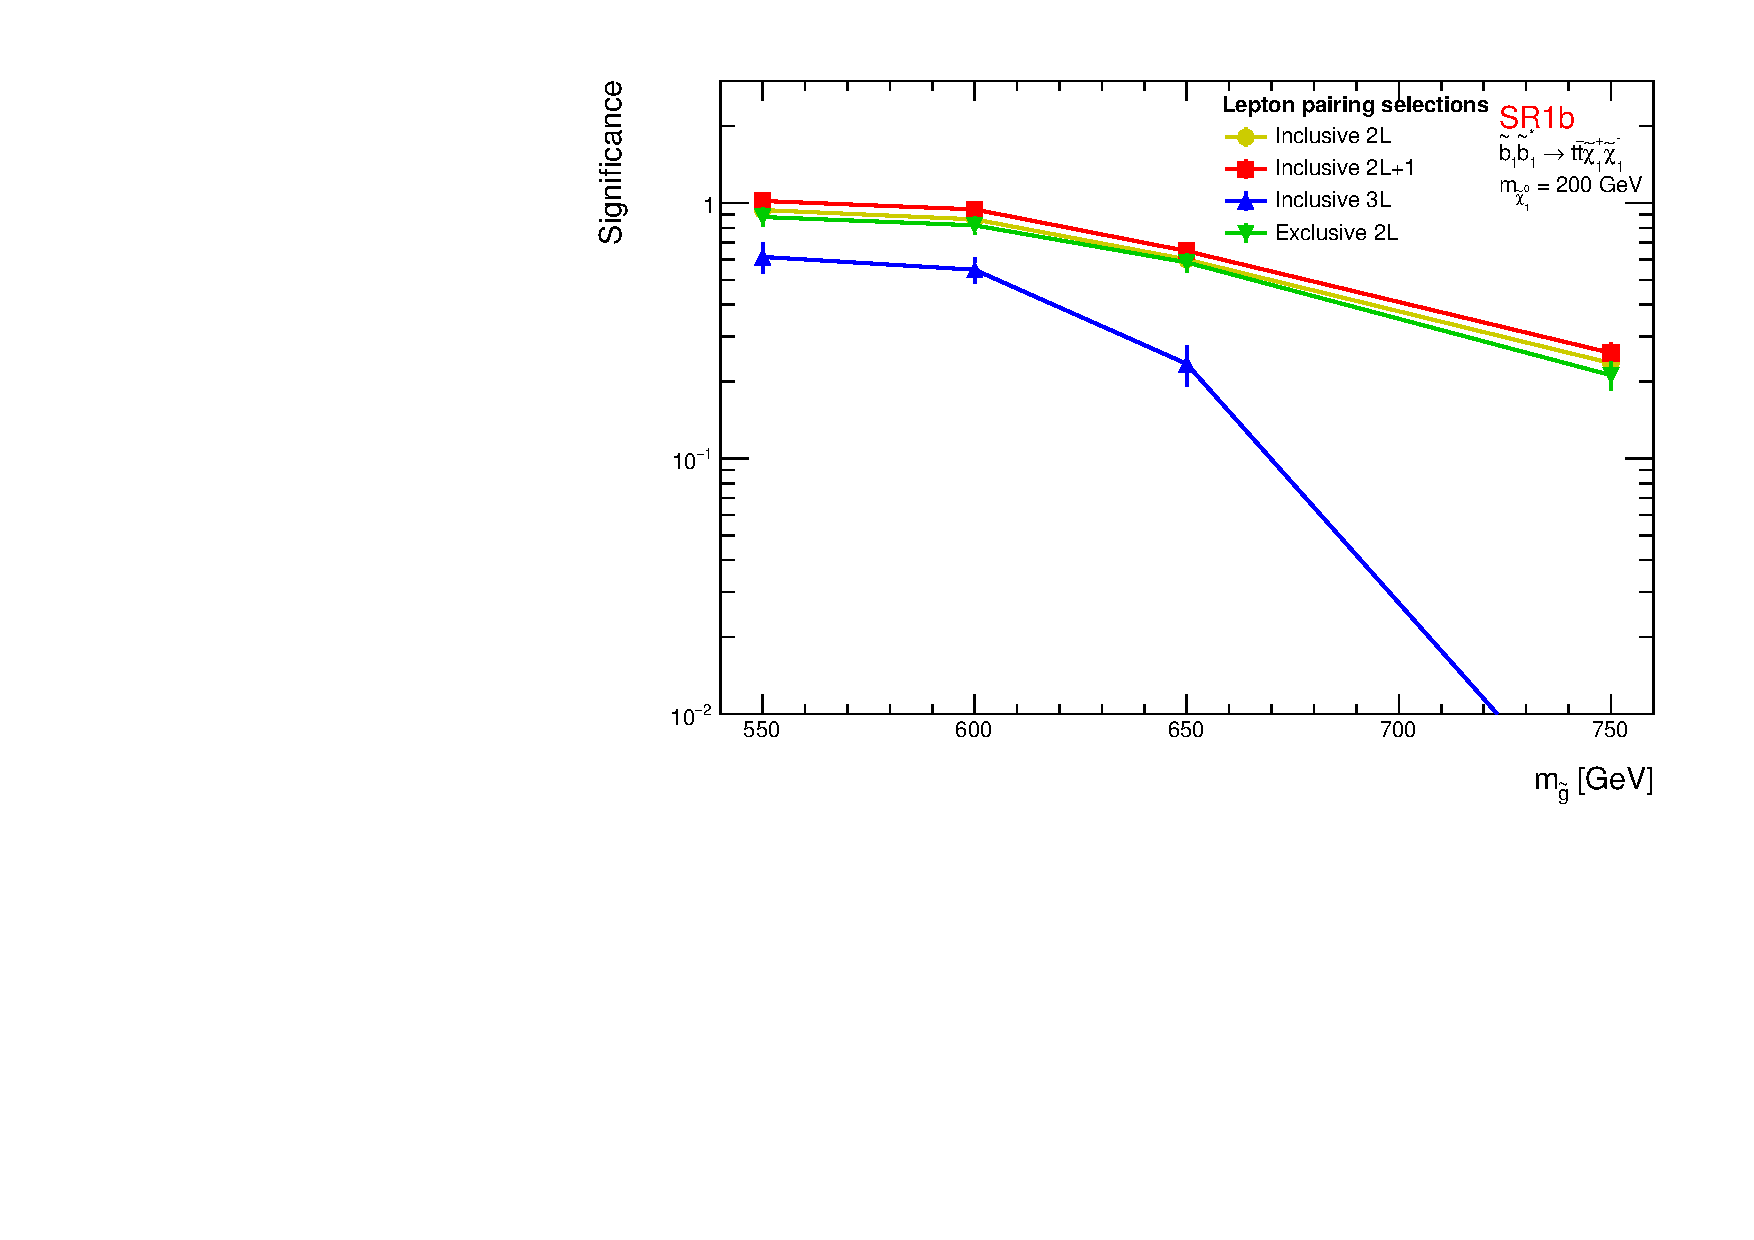
\includegraphics[width=0.49\textwidth]{PAIRING/SR1b_lepton_pairing}
  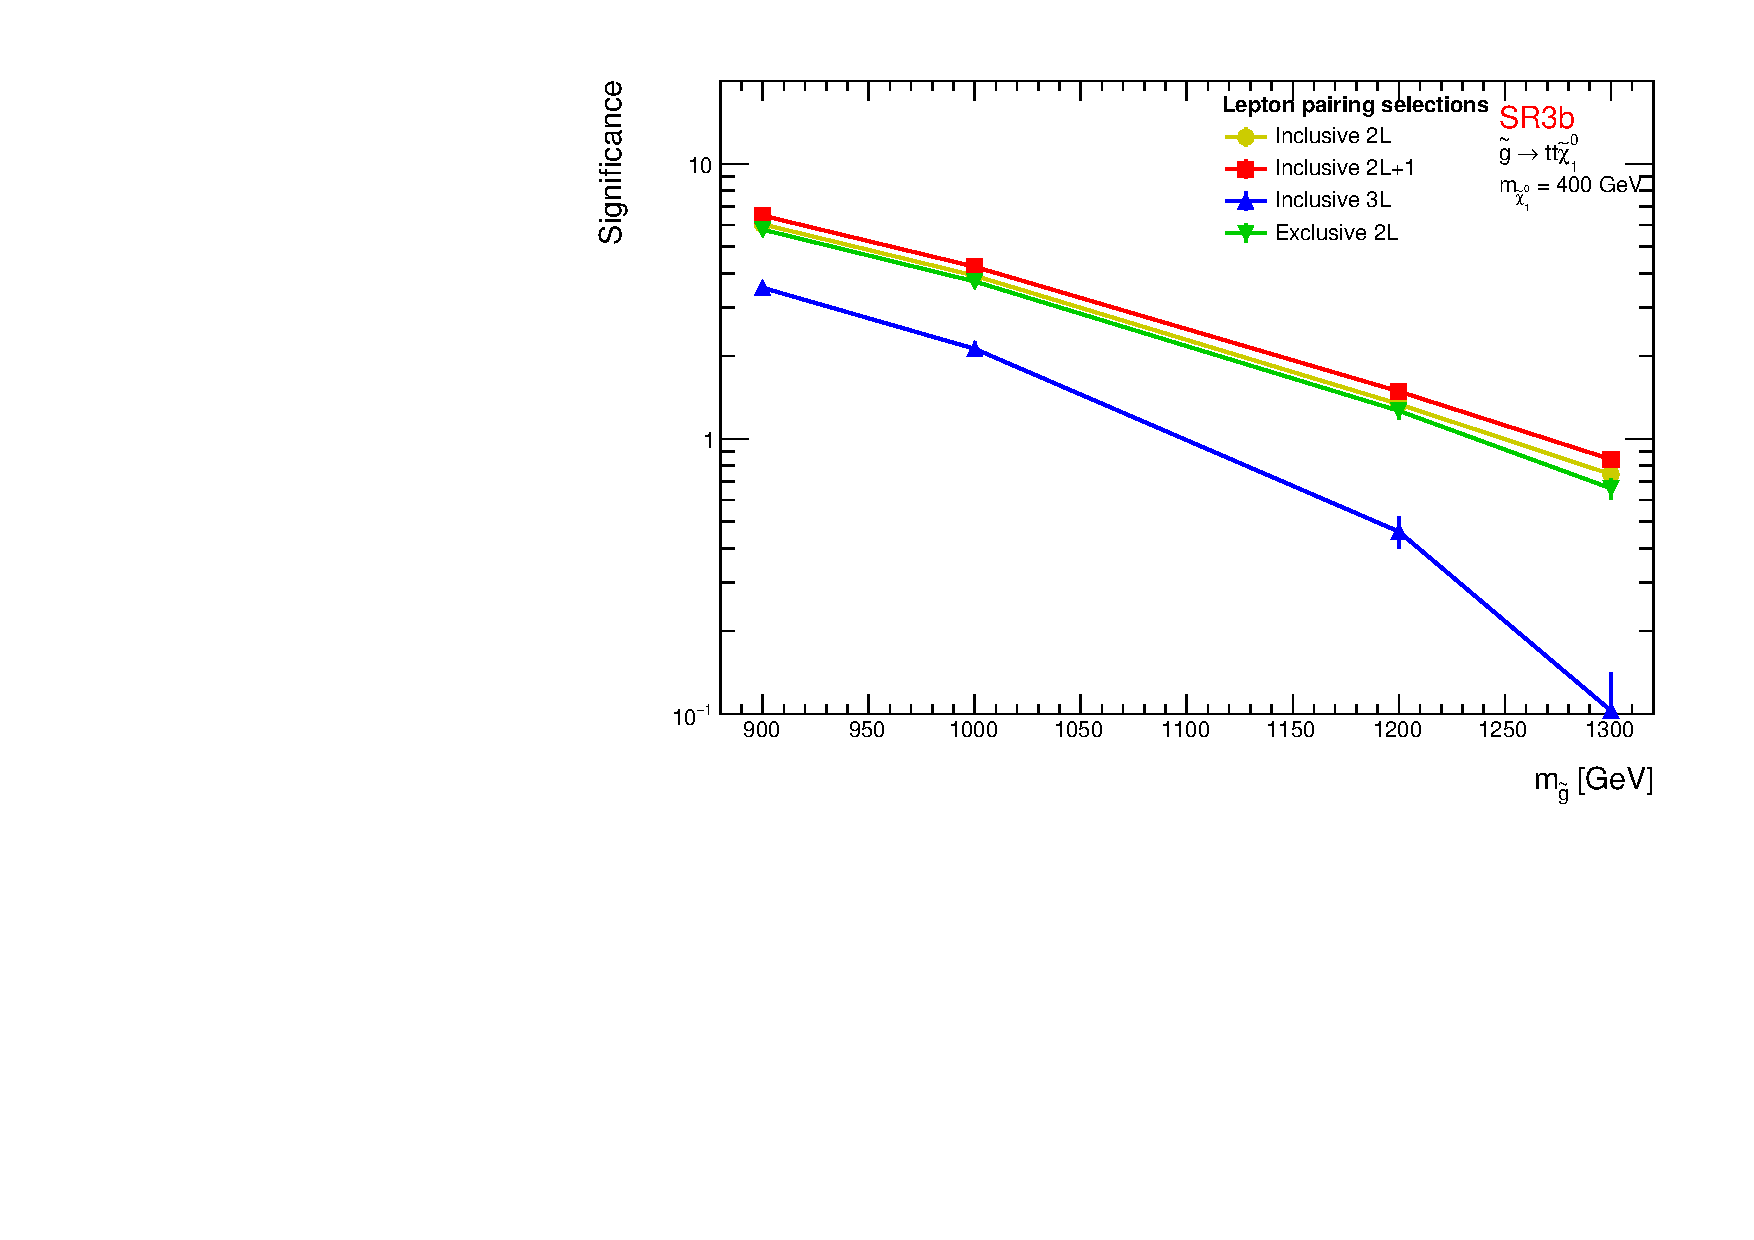
\includegraphics[width=0.49\textwidth]{PAIRING/SR3b_lepton_pairing}
  \caption{Left: Signal significances for a ``SR1b-like'' selection (cf text),  
  for several $\tilde{b}_{1}\tilde{b}_{1}^{*} \rightarrow t\bar{t}\tilde{\chi}_{1}^{+}\tilde{\chi}_{1}^{-}$ models with variable $m_{\tilde{g}}$ and fixed $m_{\chi}$ of 200 GeV. 
  Right: Signal significances for a ``SR3b-like'' selection (cf text), 
  for several $\tilde{g} \rightarrow t \bar{t} \chi_{1}$ models with variable $m_{\tilde{g}}$ and fixed $m_{\chi}$ of 400 GeV. 
  The significance is computed for different lepton pair selection strategies which are drawn in different colors in the plot.}
 \label{fig:Pairing_SR1b}
\end{figure}

\begin{figure}[!ht]
  \centering
  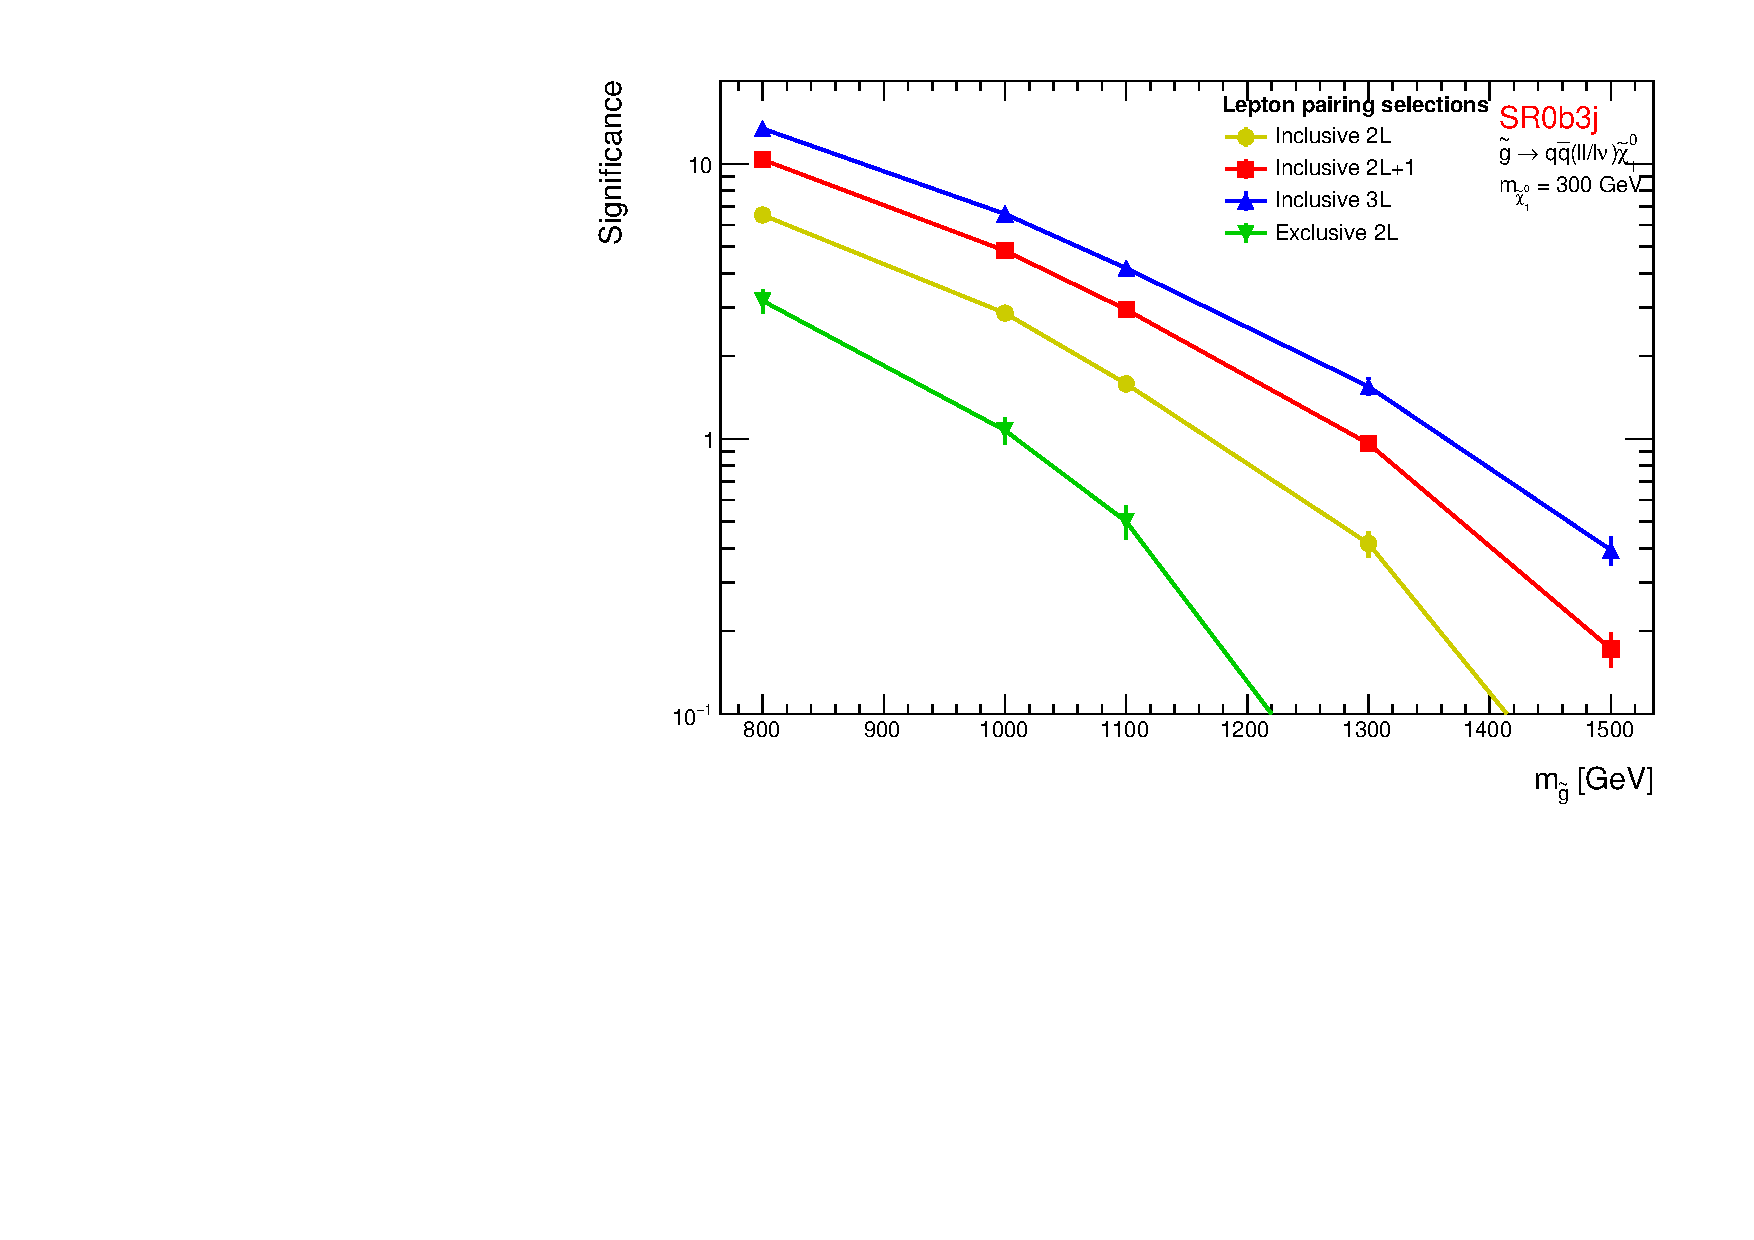
\includegraphics[width=0.49\textwidth]{PAIRING/SR0b3j_lepton_pairing}
  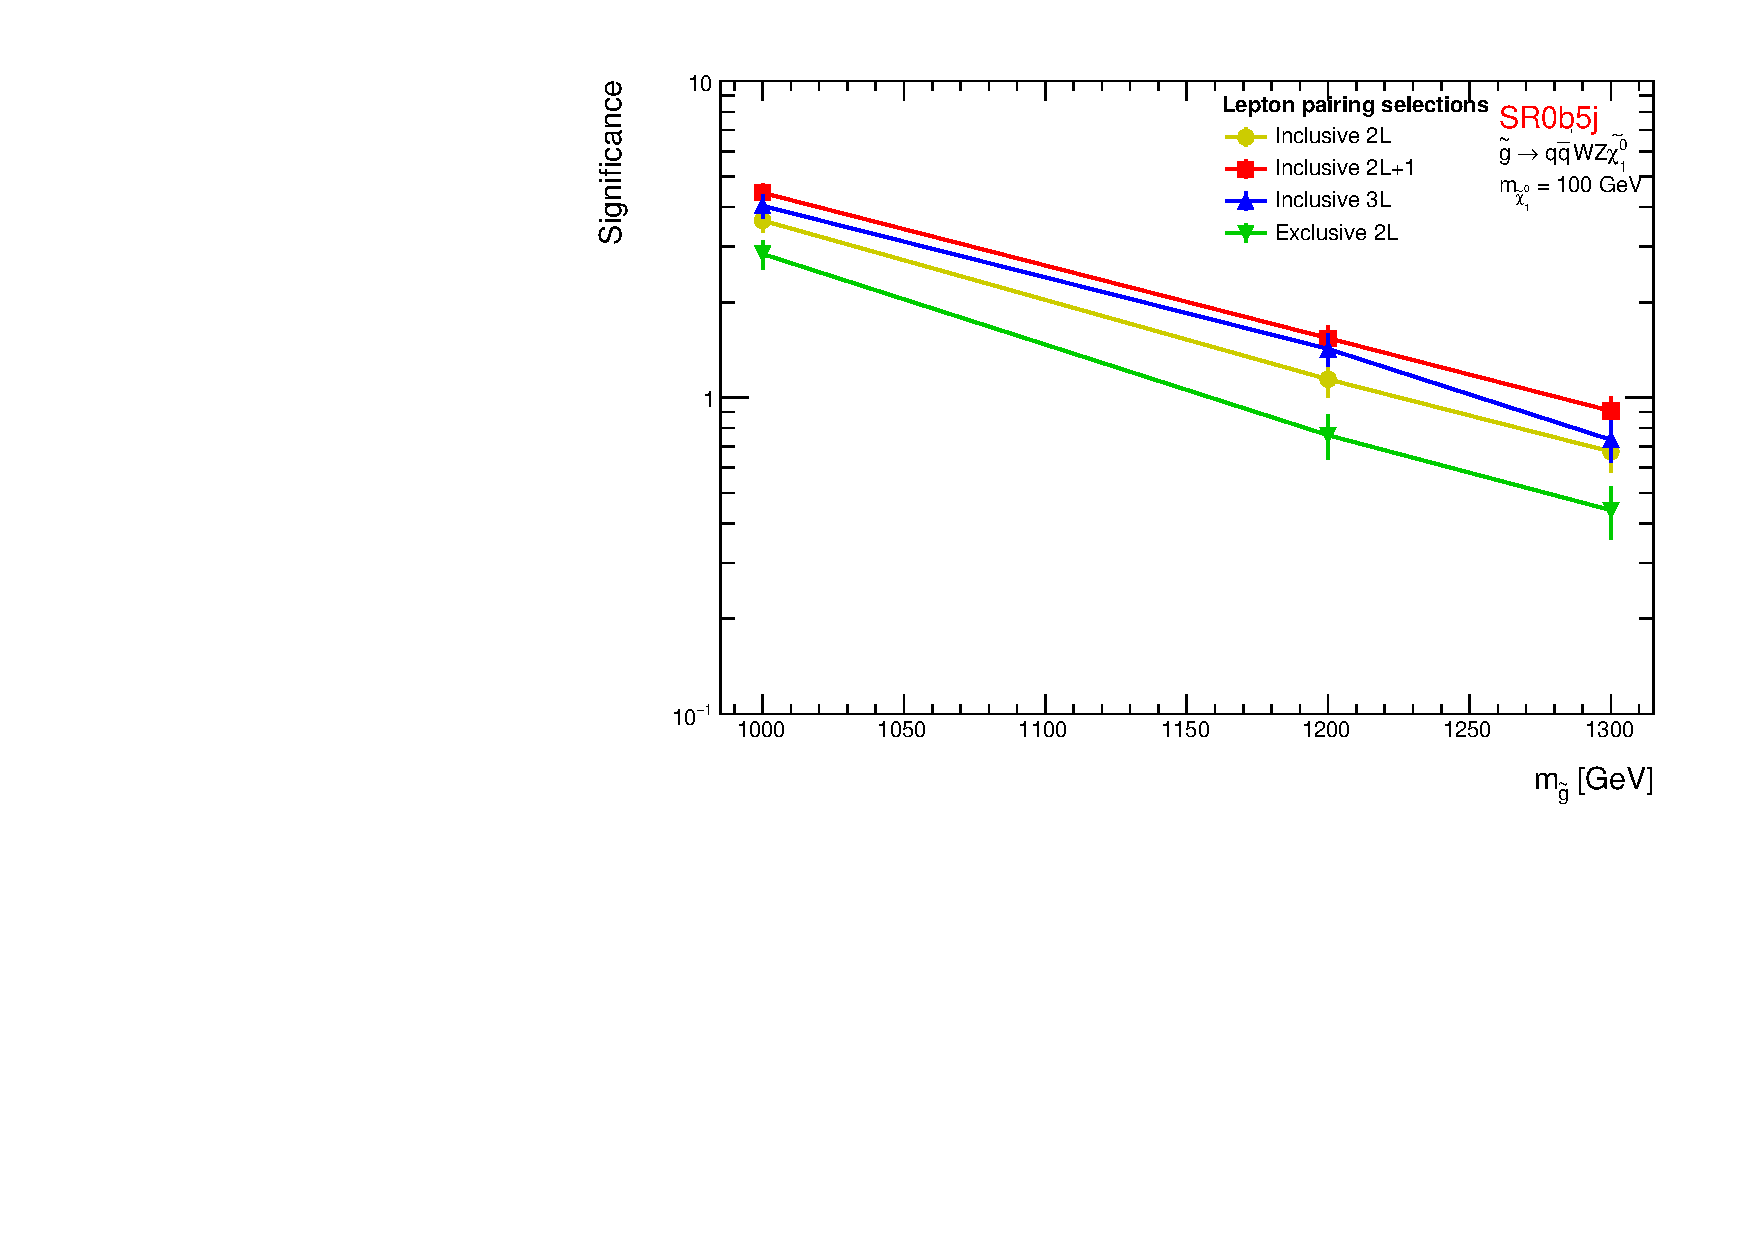
\includegraphics[width=0.49\textwidth]{PAIRING/SR0b5j_lepton_pairing}
  \caption{Left: Signal significances for a ``SR0b3j-like'' selection (cf text) 
  for several $\tilde{g} \rightarrow q\bar{q}(ll/l\nu)\tilde{\chi}_{1}^{0}$ models with variable $m_{\tilde{g}}$ and fixed $m_{\chi}$ of 300 GeV. 
Right: Signal significances for a ``SR0b5j-like'' selection (cf text) 
for several $\tilde{g} \rightarrow qqWZ\tilde{\chi}_{1}^{0}$ models with variable $m_{\tilde{g}}$ and fixed $m_{\chi}$ of 100 GeV. 
The significance is computed for different lepton pair selection strategies which are drawn in different colors in the plot.}
  \label{fig:Pairing_SR0b3j}
\end{figure}

Figure~\ref{fig:Pairing_SR1b} and~\ref{fig:Pairing_SR0b3j} show the signal significance for event selections
\footnote{All regions require $\ge 2 $ same-sign leptons; 
SR3b = $\ge 3$ $b$-jets + $\ge 6$ jets, SR1b = $\ge 1$ $b$-jet + $\ge 4$ jets + $\met>150$ GeV + $\meff>500$ GeV, 
SR0b3j = $b$-jet veto + $\ge 3$ jets + $\met>200$ GeV + $\meff>400$ GeV, SR0b5j = $b$-jet veto + $\ge 5$ jets + $\met>100$ GeV + $\meff>400$ GeV.} 
close to the final signal regions definitions (cf section~\ref{sec:SignalRegDef}), 
for the four different lepton pairing selections varying the gluino mass and a fixed neutralino mass. 
The ``inclusive 2L+1'' option shows the highest significance for almost all of the mass points investigated.
Since this pairing option is the most inclusive one in all signal regions, the event yields are higher 
with respect to the other options leading to a better exclusion strength for most signal scenarios.\\
The only exception is in SR0b3j where the Inclusive 3L is more efficient. 
This motivates the final decision of requiring at least 3 leptons in this signal region (cf section\~ref{sec:SignalRegDef}).\\ 

\subsubsection{Validation of the \pt cuts for the leading, sub-leading and 3rd lepton}

Since the ``inclusive 2L+1'' lepton pairing selection turned out to be the most significant one in most scenarios, this configuration has been used to investigate also the impact of changes in the \pt cuts of the lepton on the analysis sensitivity. Therefore several \pt cuts for the signal leptons have been tested independently. One additional configuration which was also tested in which is to apply only the baseline requirements on the third lepton if already two signal leptons have been found in the event. 

\begin{figure}[!ht]
  \centering
  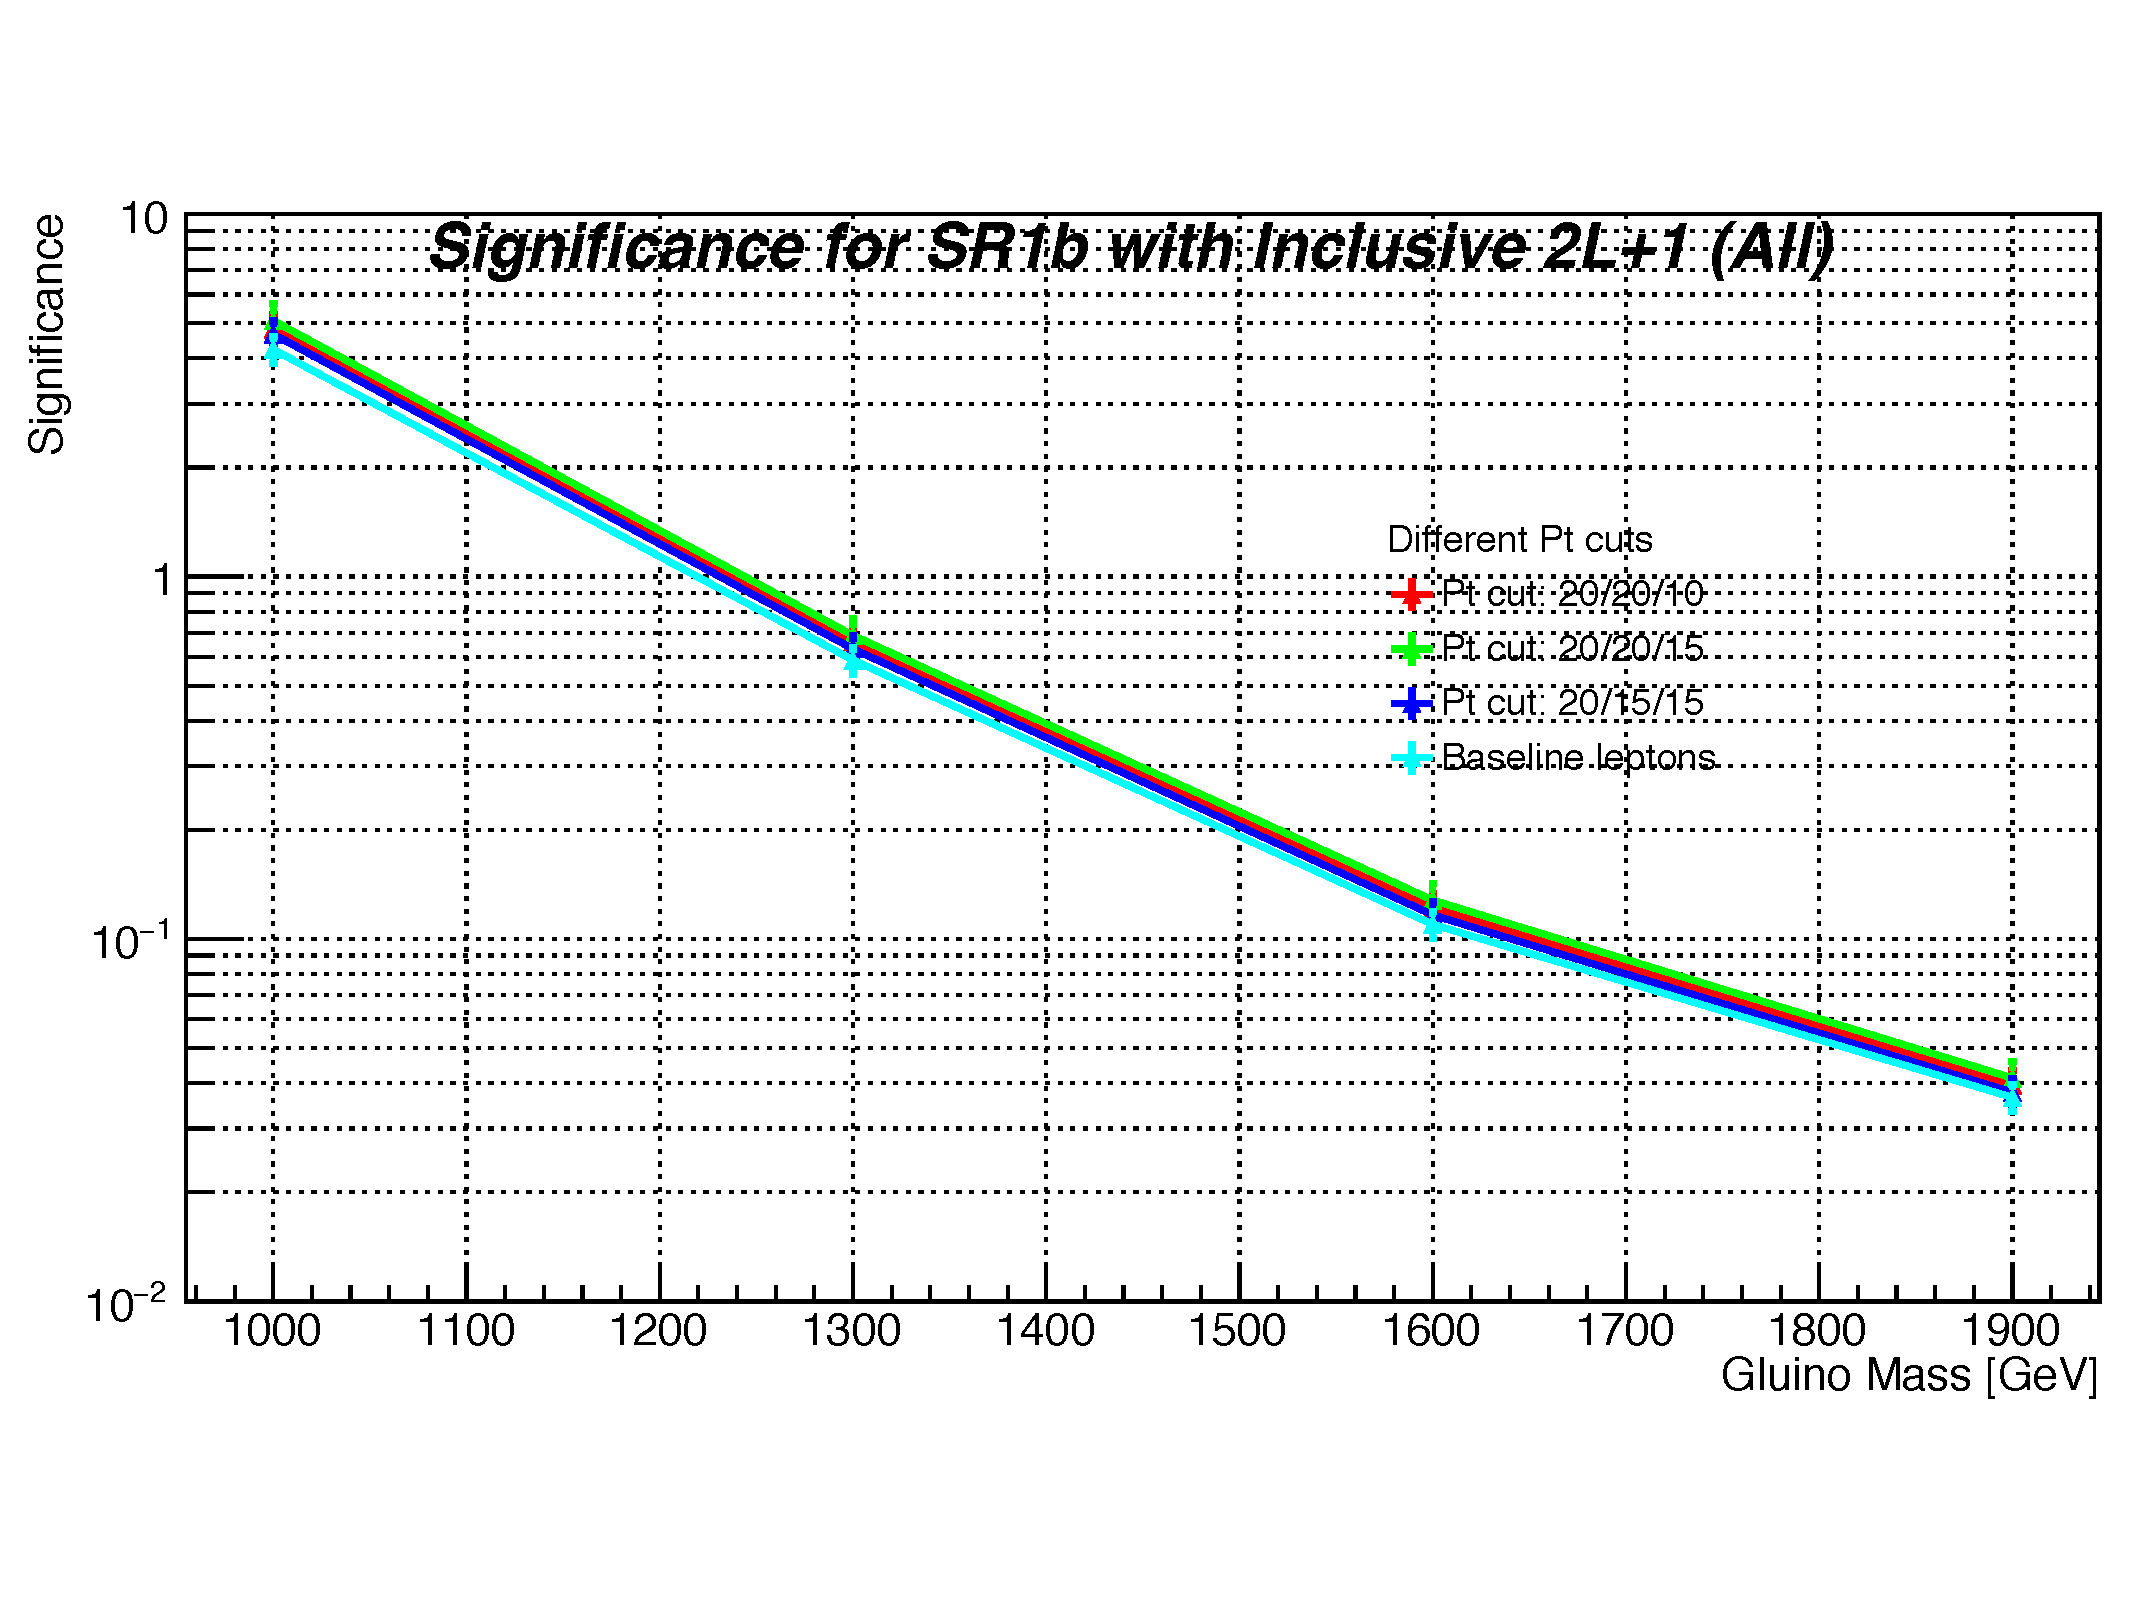
\includegraphics[width=0.49\textwidth, page=1]{PAIRING/Pt_SR1b_SR3b.pdf}
  \includegraphics[width=0.49\textwidth, page=2]{PAIRING/Pt_SR1b_SR3b.pdf}
  \caption{Significances of the signal region SR1b and SR3b for $\tilde{g} \rightarrow t \bar{t} \chi_{1}$ models with variable $m_{\tilde{g}}$ and fixed $m_{\chi}$ of 100 GeV. The significance is computed for different \pt cuts on 1st, 2nd and 3rd lepton. The significances are also shown for $\pt(1st, \, 2nd, \, 3rd) = 20, \, 20, \, 10 $ GeV, relaxing the requirements on the third lepton to baseline-cuts.}
  \label{fig:Pt_SR1b_SR3b}
\end{figure}

Figure~\ref{fig:Pt_SR1b_SR3b} shows the significances of SR1b and SR3b (as defined in previous section) for different \pt cuts on first, second and third leptons. 
The significances are also shown for $\pt({\text 1st, 2nd, 3rd}) = 20, \, 20, \, 10 $ GeV but relaxing the requirements on the third lepton to baseline-cuts. 
The observed significances show only small dependencies on changes of the $p_T$ cuts. 
Also relaxing the requirements of the third lepton to the baseline definition has no big impact on the sensitivity of the analysis. 
Therefore a modification of the nominal lepton selection criteria would not bring a substantial benefit to the analysis sensitivity. 

%% \subsubsection{Validation of the jet \pt requirements in signal regions with a $b$ veto}
%% this section has been moved, to be after the SR definitions

\subsection{Data-MC comparisons}

In order to validate the various choices made regarding the object definitions and event selection, 
check their sensible behavior and their reasonable modelling in the simulations, 
we looked at the distributions of several kinematic variables obtained with the available 13 TeV data. 
Figures~\ref{fig:dataMC_2lep}-\ref{fig:dataMC_metmeff} show such selected distributions in data compared to MC. The background distributions are taken directly from MC with no data-driven estimation of the charge flip or non-prompt lepton backgrounds.

Figure~\ref{fig:dataMC_2lep} shows the dilepton invariant mass distributions for both OS and SS dilepton events, 
computed with the two leading $p_T$ leptons. 
A very good agreement with MC is observed in the OS channels, with a clear $Z$-boson mass peak in the $ee$ and $\mu\mu$ channels. 
In the SS channels, the $Z$-boson mass peak is also observed in the $ee$ channel due to electron charge mis-identification, with MC overestimating data by 20-30\%. 
An accumulation of events at the $Z$-boson mass is also observed in the SS $e\mu$ and $\mu\mu$ channels due to three-lepton events 
from either $Z$+jets with a fake lepton or from $WZ$ production.  

Lepton distributions are shown in Figures~\ref{fig:dataMC_lep1}-\ref{fig:dataMC_lep2}, with a reasonable data-MC agreement except at low lepton $\pt$ where some discrepancies and accumulation of events involving fake leptons ($Z$+jets, $W$+jets, $\ttbar$) are observed. Jet and $b$-jet distributions are shown in Figures~\ref{fig:dataMC_jet}-\ref{fig:dataMC_bjet} and Figure~\ref{fig:dataMC_metmeff} shows the $\met$ and $m_{\rm eff}$ distributions.

\begin{figure}[htb!]
\centering
{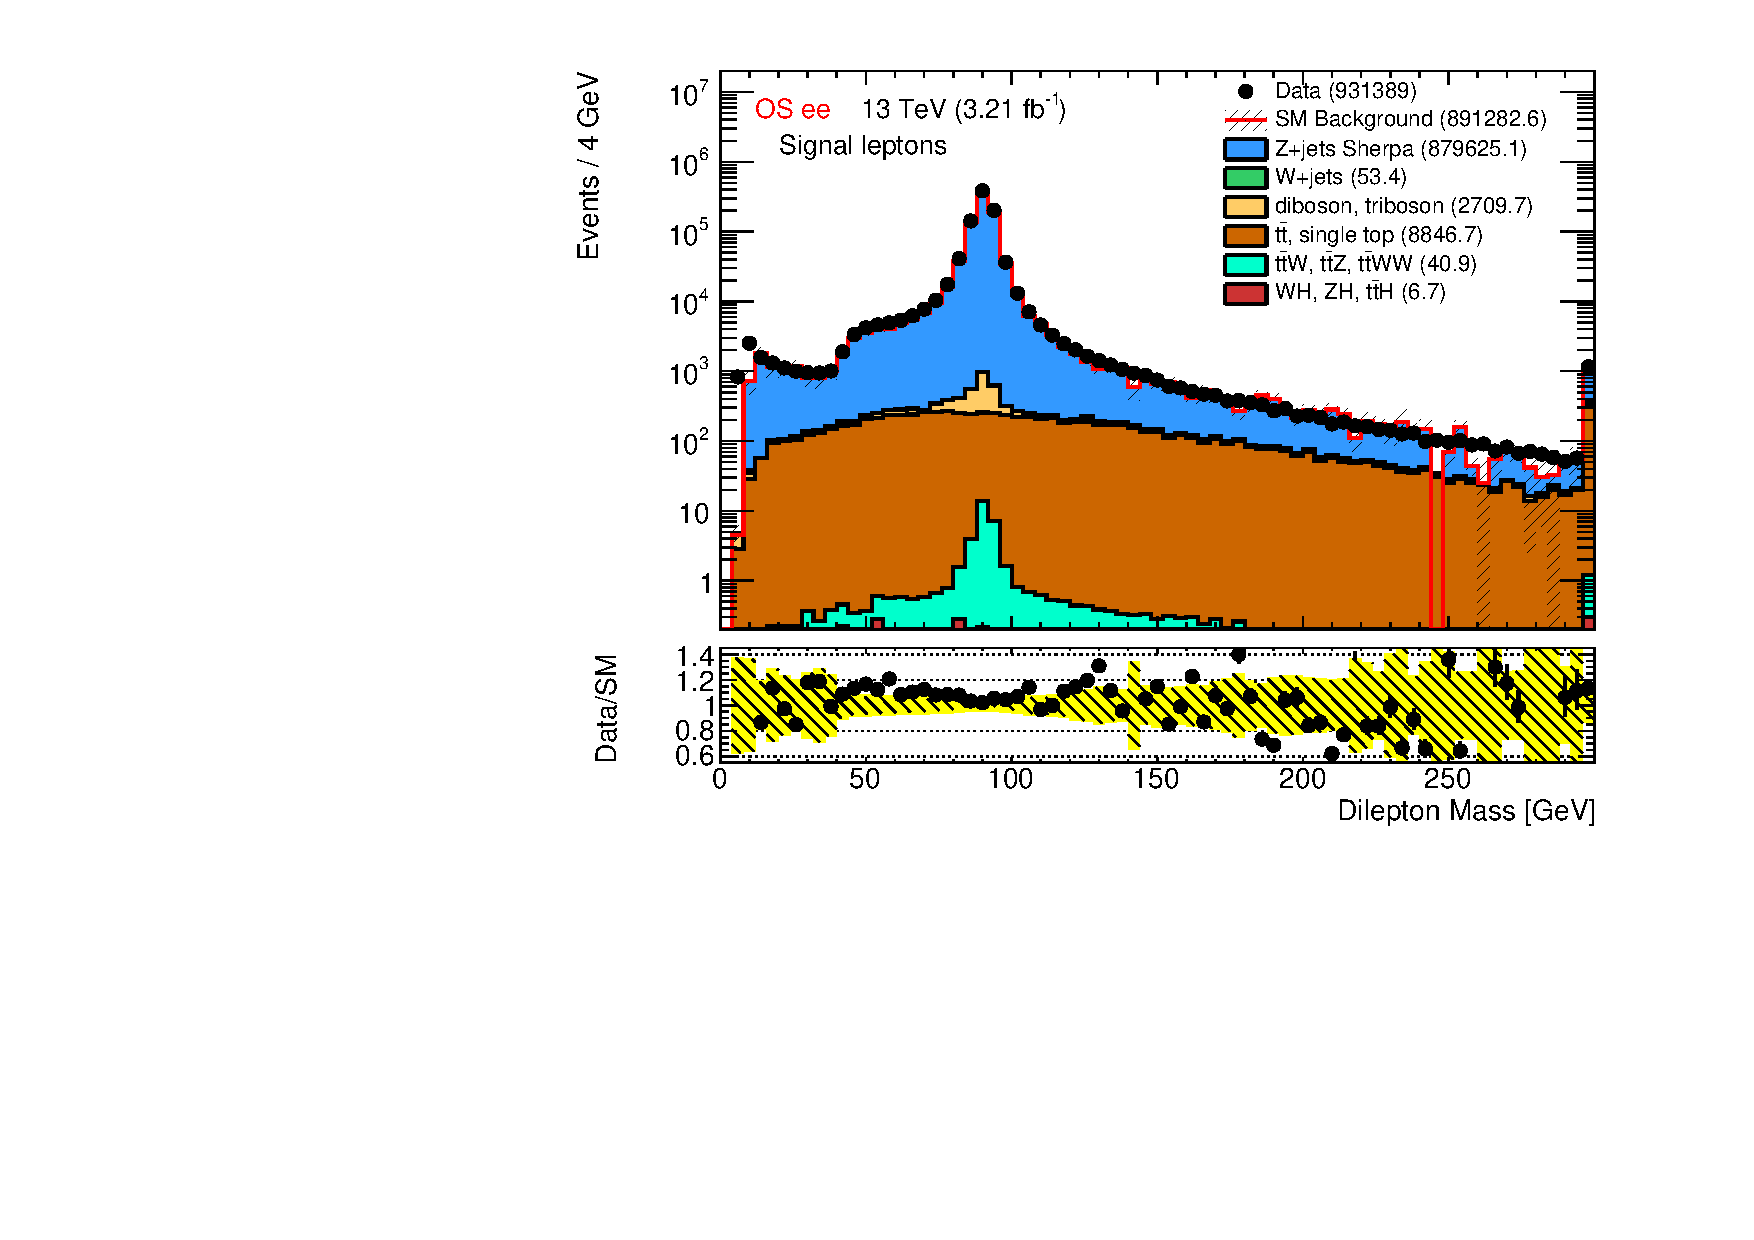
\includegraphics[width=0.49\textwidth]{DATAMC/Mll_afterlepton_OSee_0_physics.pdf}}
{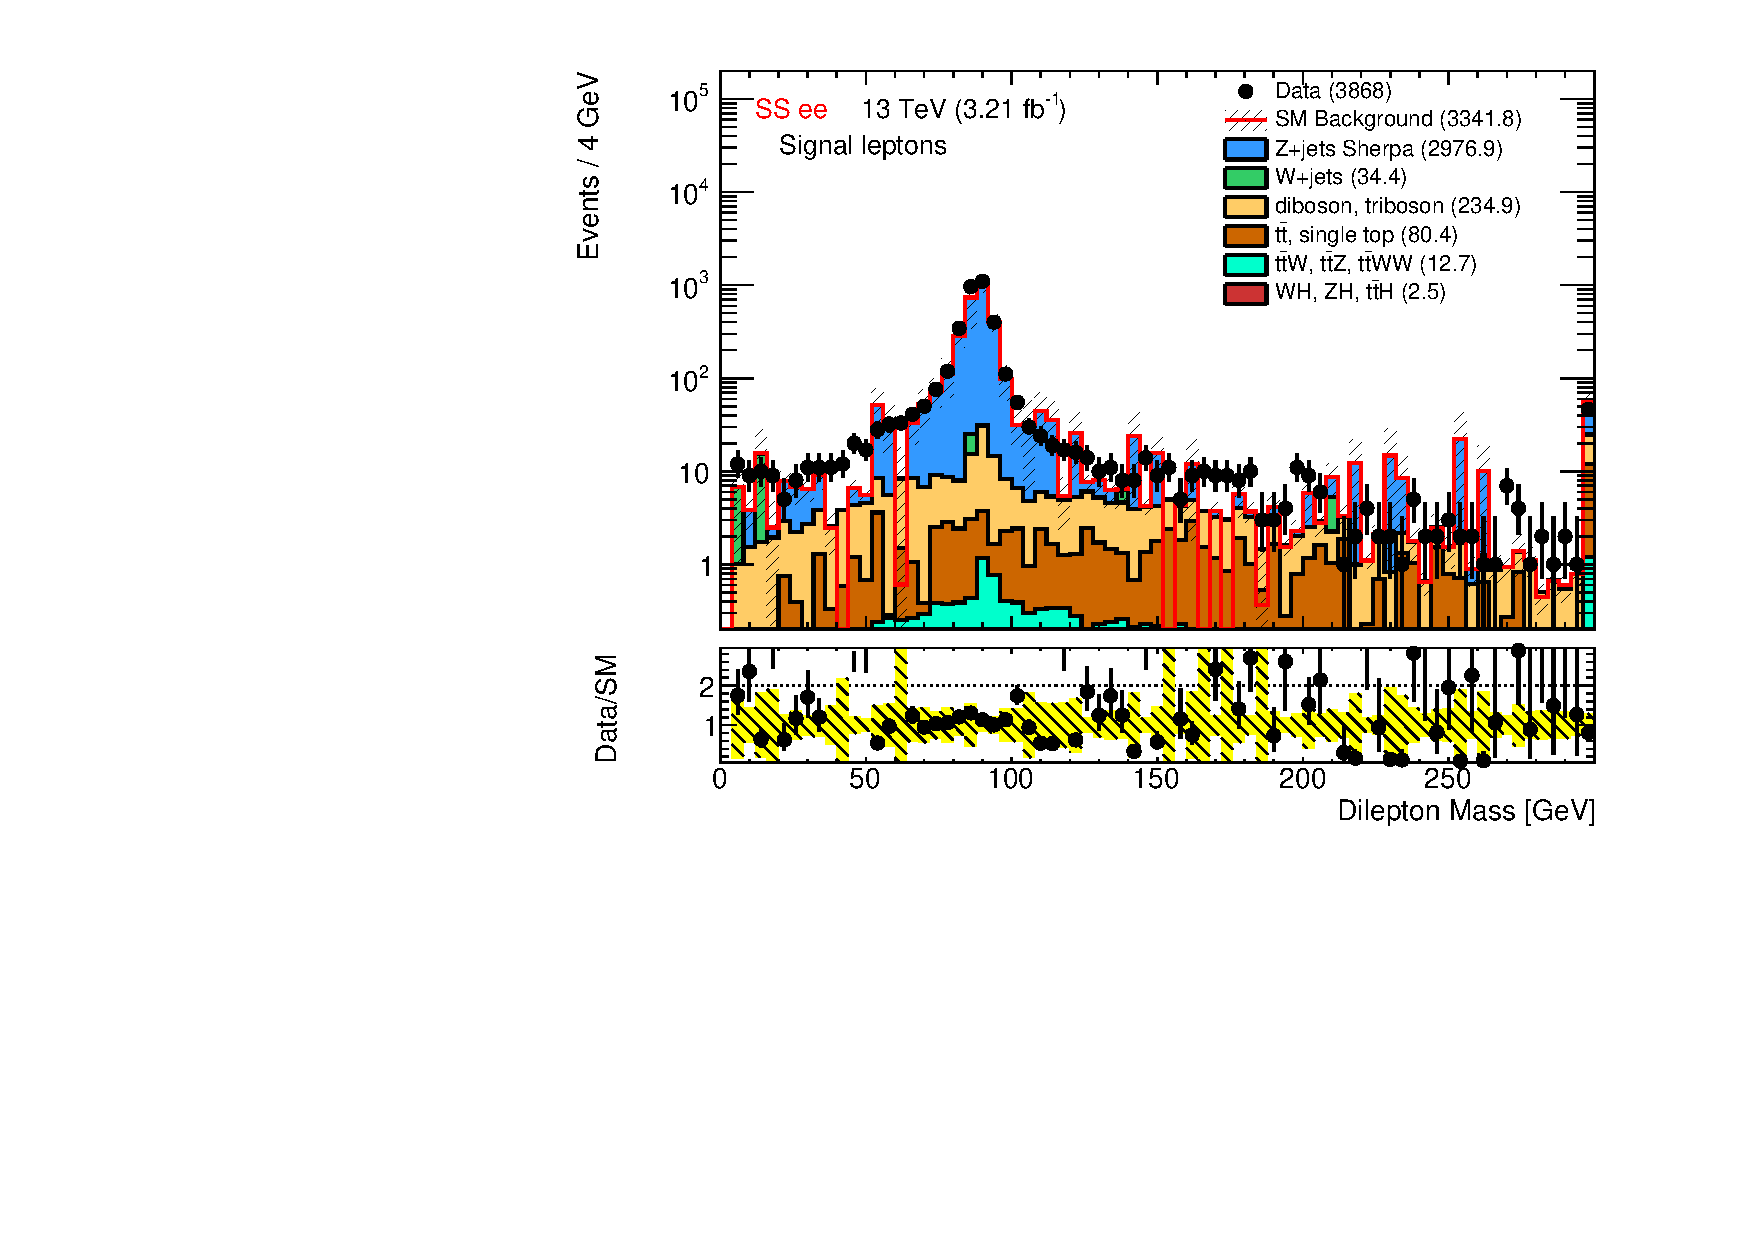
\includegraphics[width=0.49\textwidth]{DATAMC/Mll_afterlepton_SSee_0_physics.pdf}}
{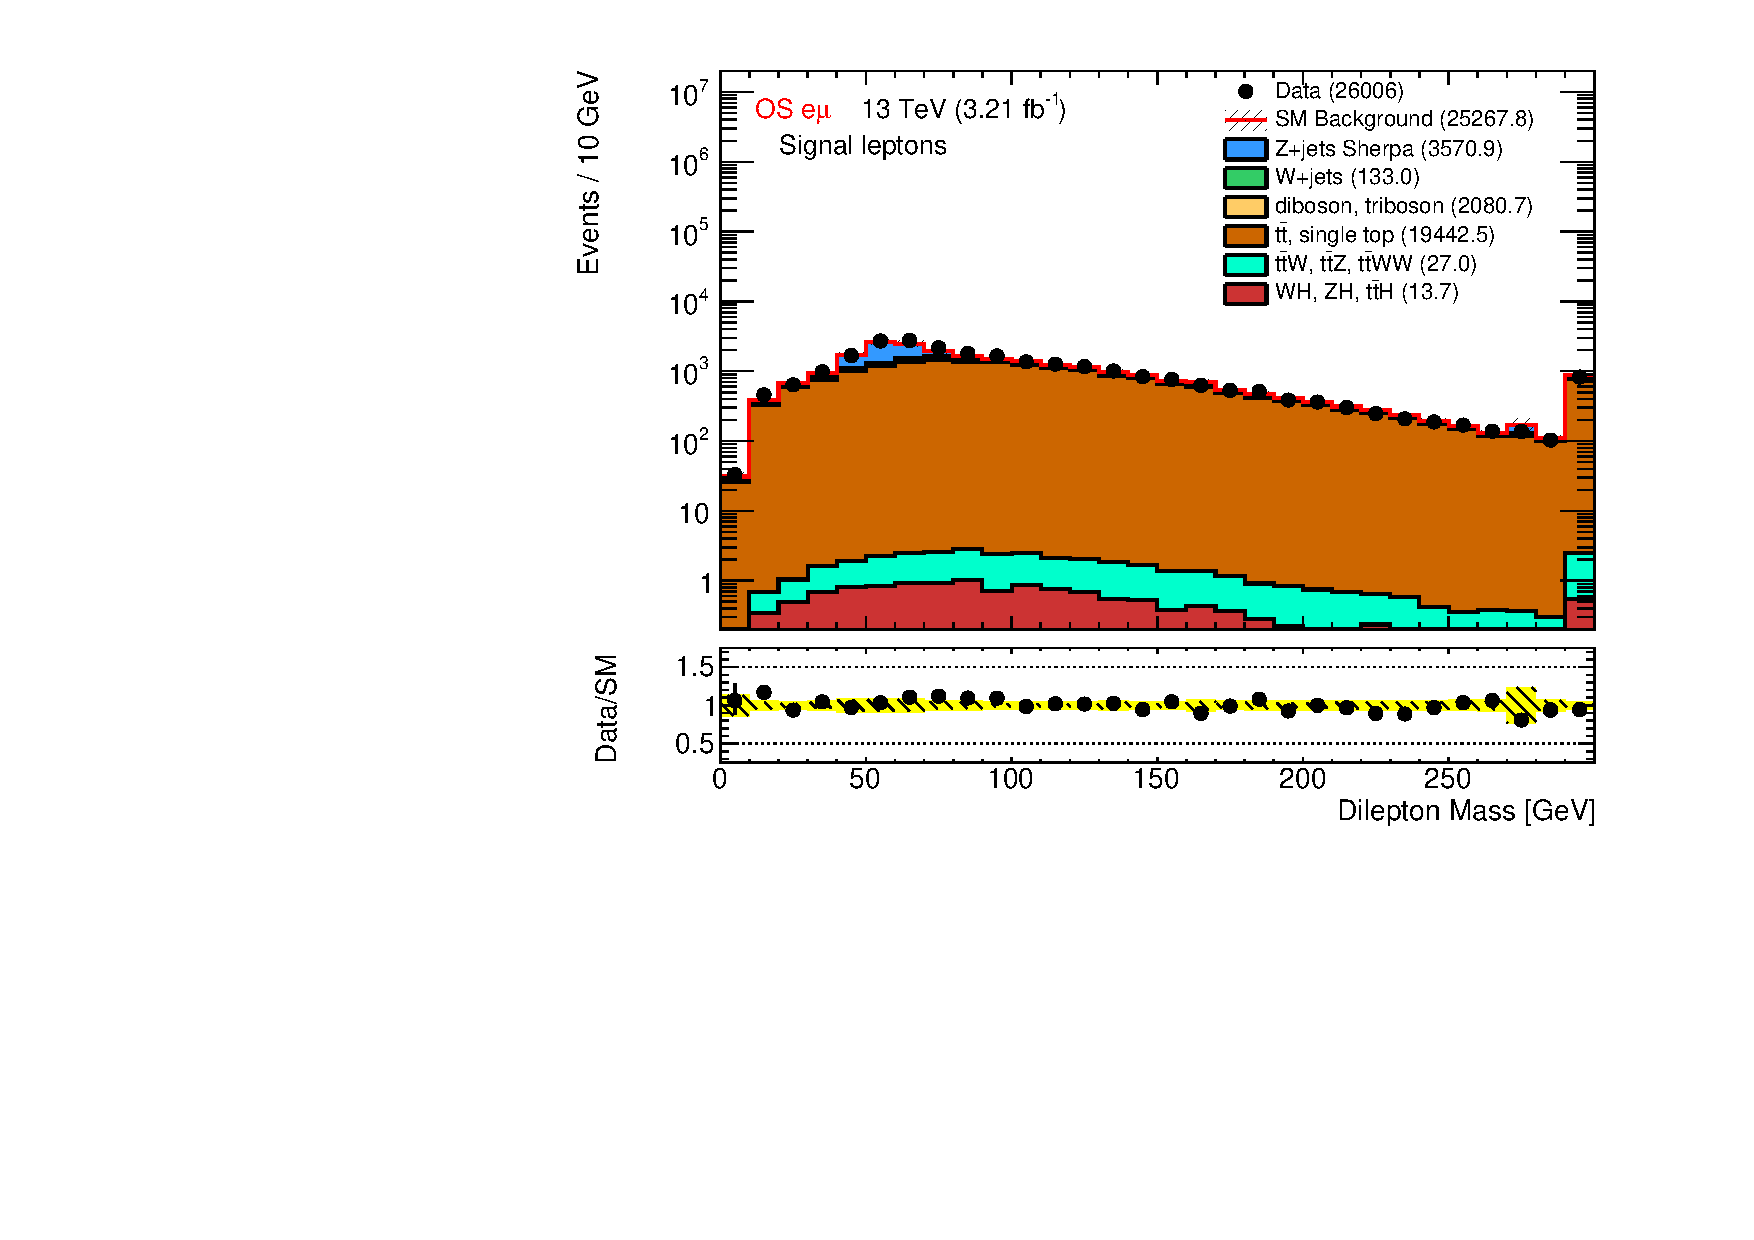
\includegraphics[width=0.49\textwidth]{DATAMC/Mll_afterlepton_OSem_0_physics.pdf}}
{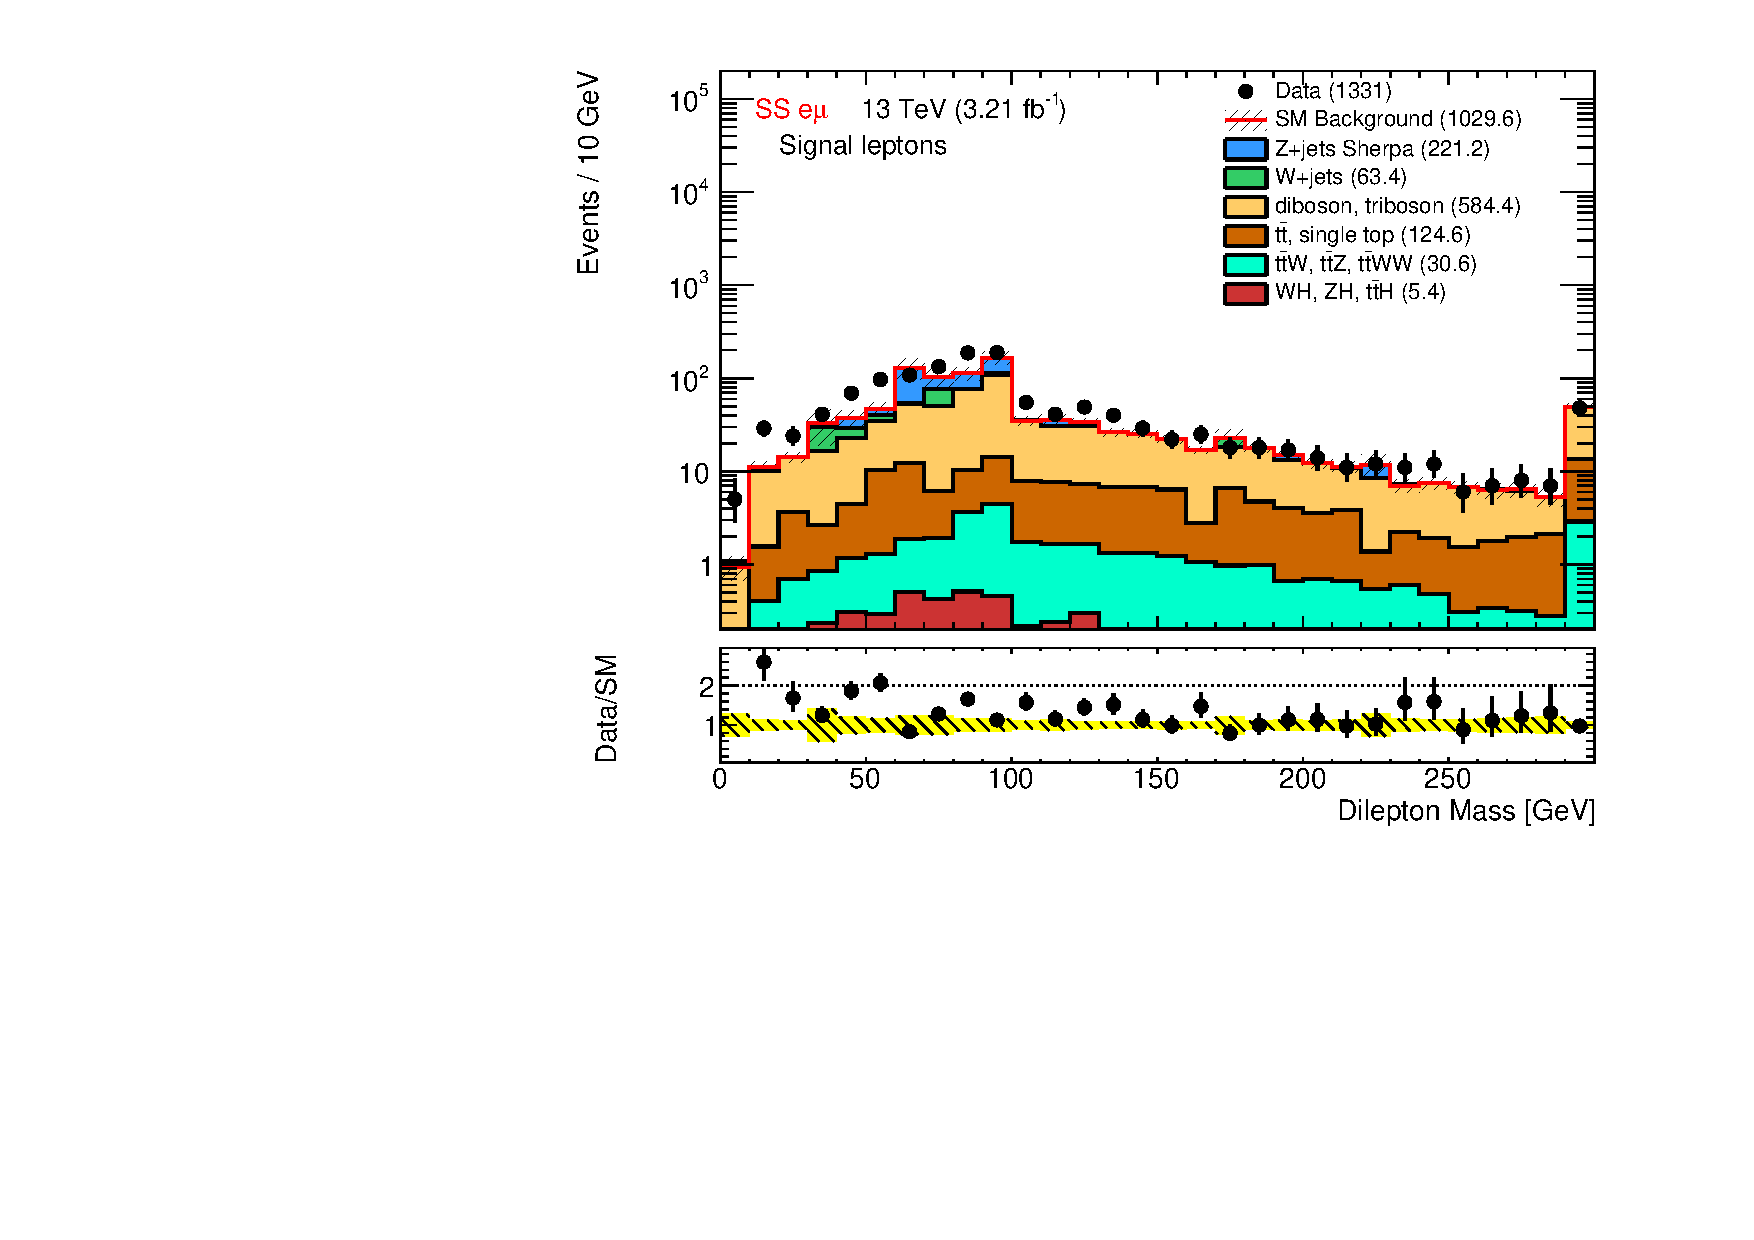
\includegraphics[width=0.49\textwidth]{DATAMC/Mll_afterlepton_SSem_0_physics.pdf}}
{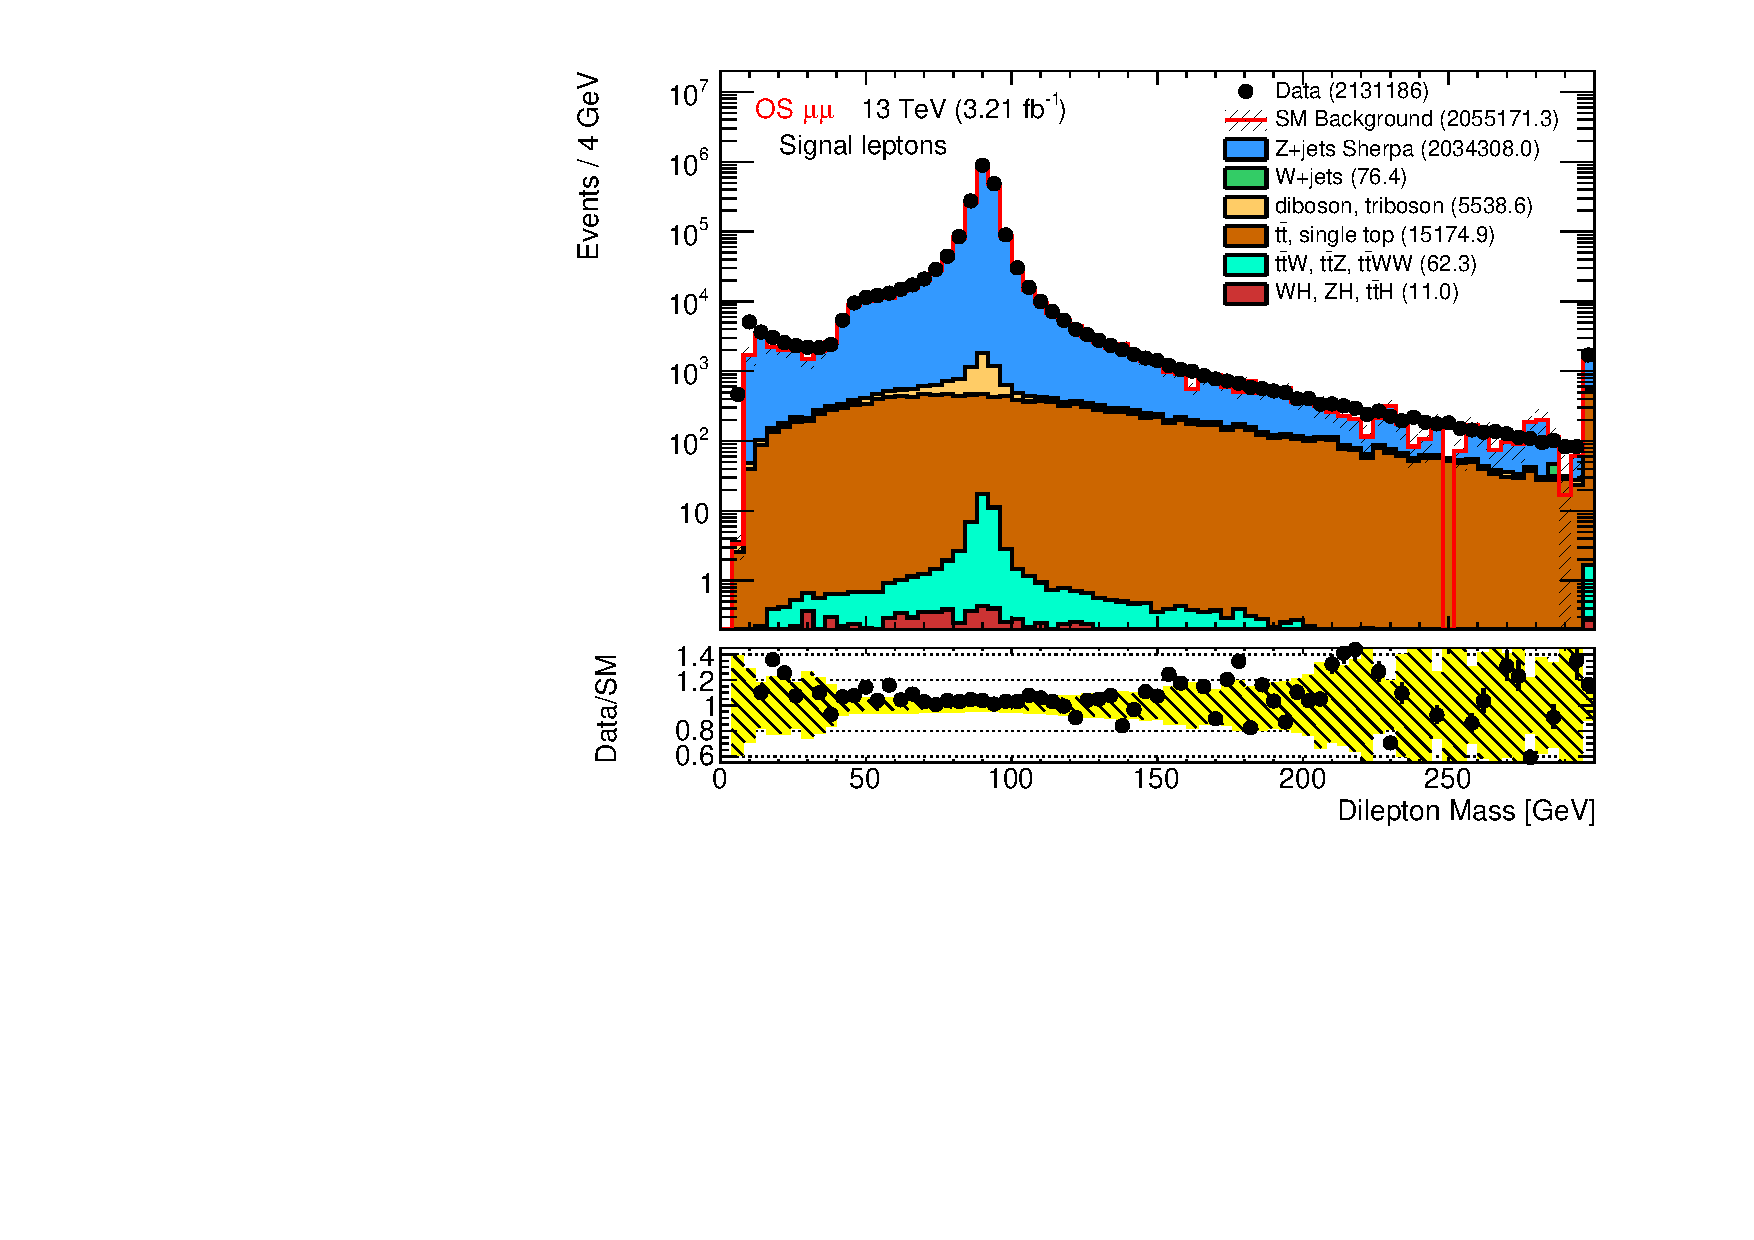
\includegraphics[width=0.49\textwidth]{DATAMC/Mll_afterlepton_OSmm_0_physics.pdf}}
{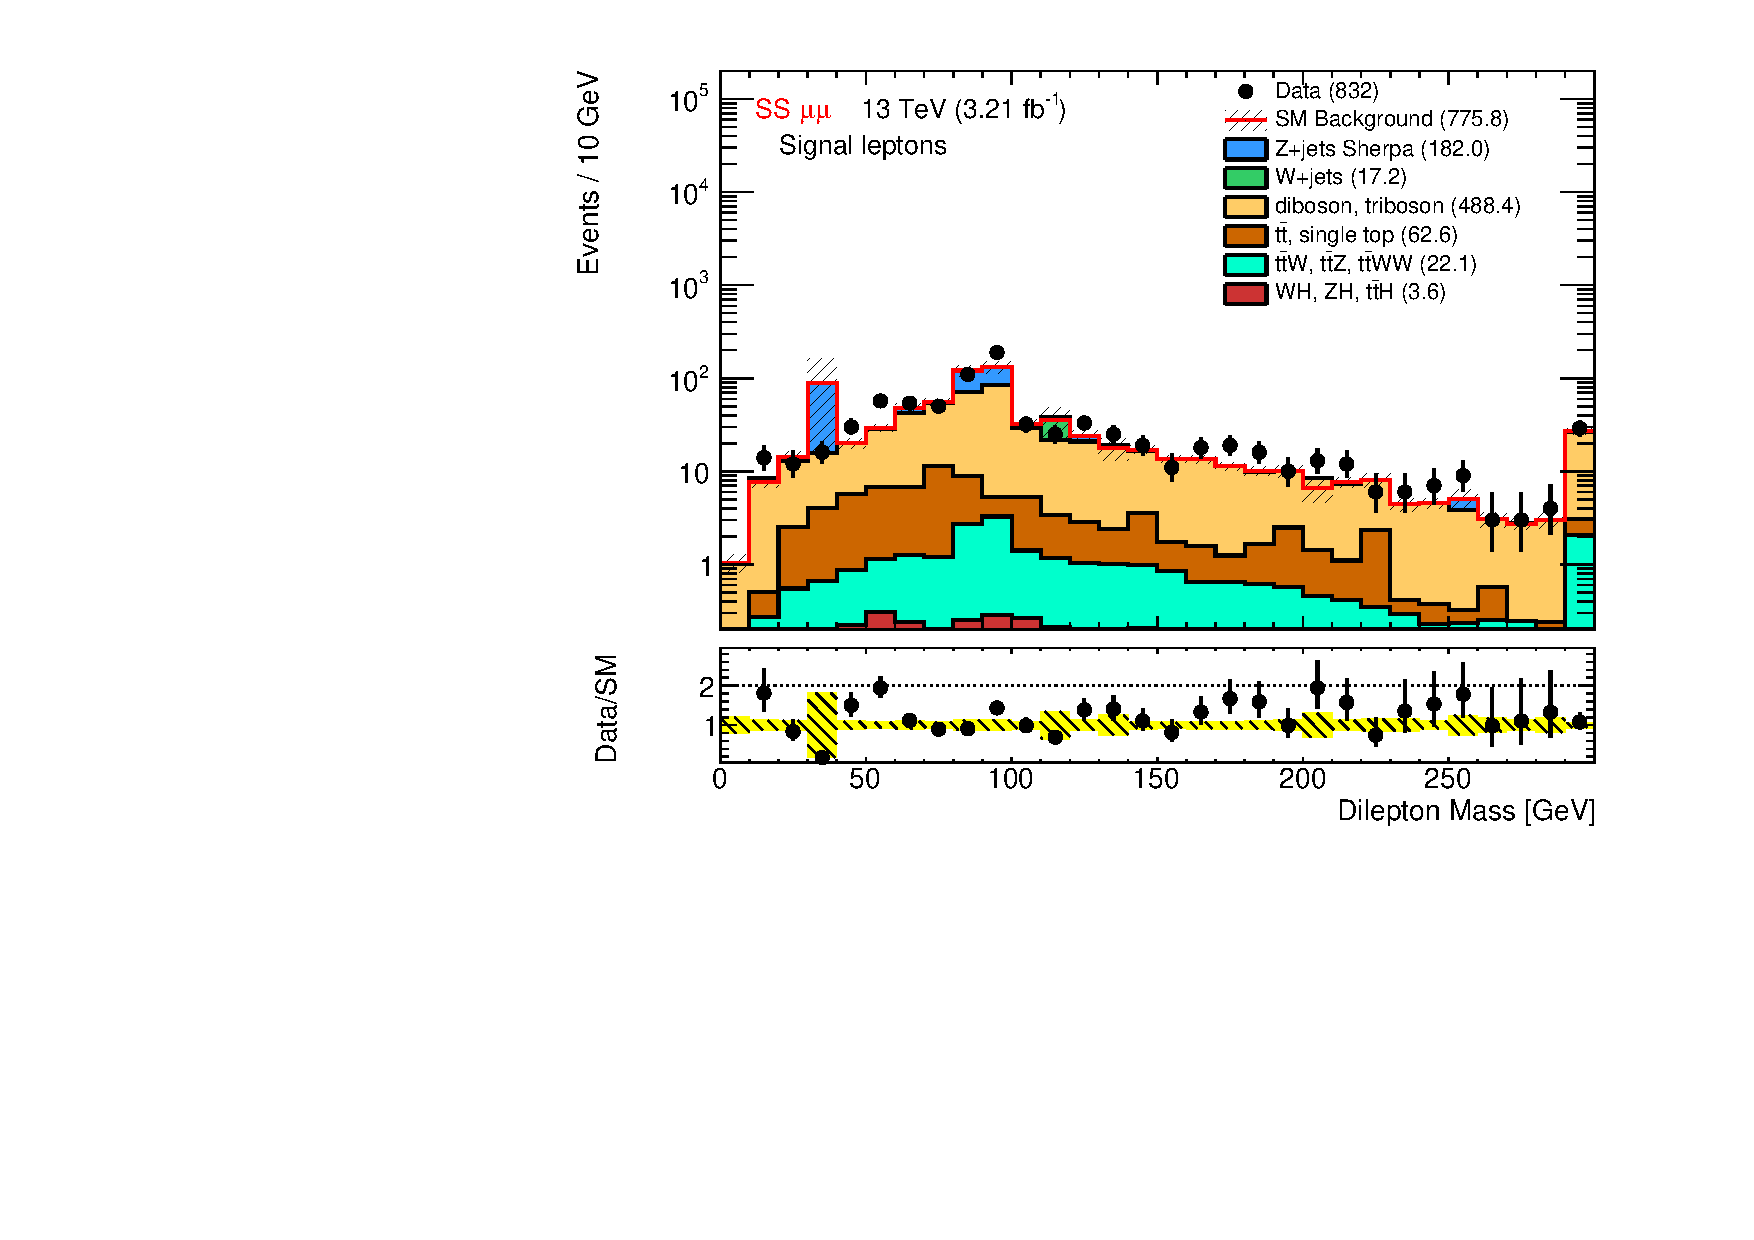
\includegraphics[width=0.49\textwidth]{DATAMC/Mll_afterlepton_SSmm_0_physics.pdf}}
\caption{Dilepton invariant mass distributions for opposite-sign (left) and same-sign (right) pairs for events selected in the $ee$ (top), $e\mu$ (center) and $\mu\mu$ (bottom) channels, computed with the two leading $p_T$ leptons. The background contribution is taken directly from MC with no data-driven estimation of the background with fake and non-prompt leptons or charge mis-identification. No low-mass Drell-Yan sample is included. Only luminosity and MC statistical uncertainties are included.
}
\label{fig:dataMC_2lep}
\end{figure}

\begin{figure}[htb!]
\centering
{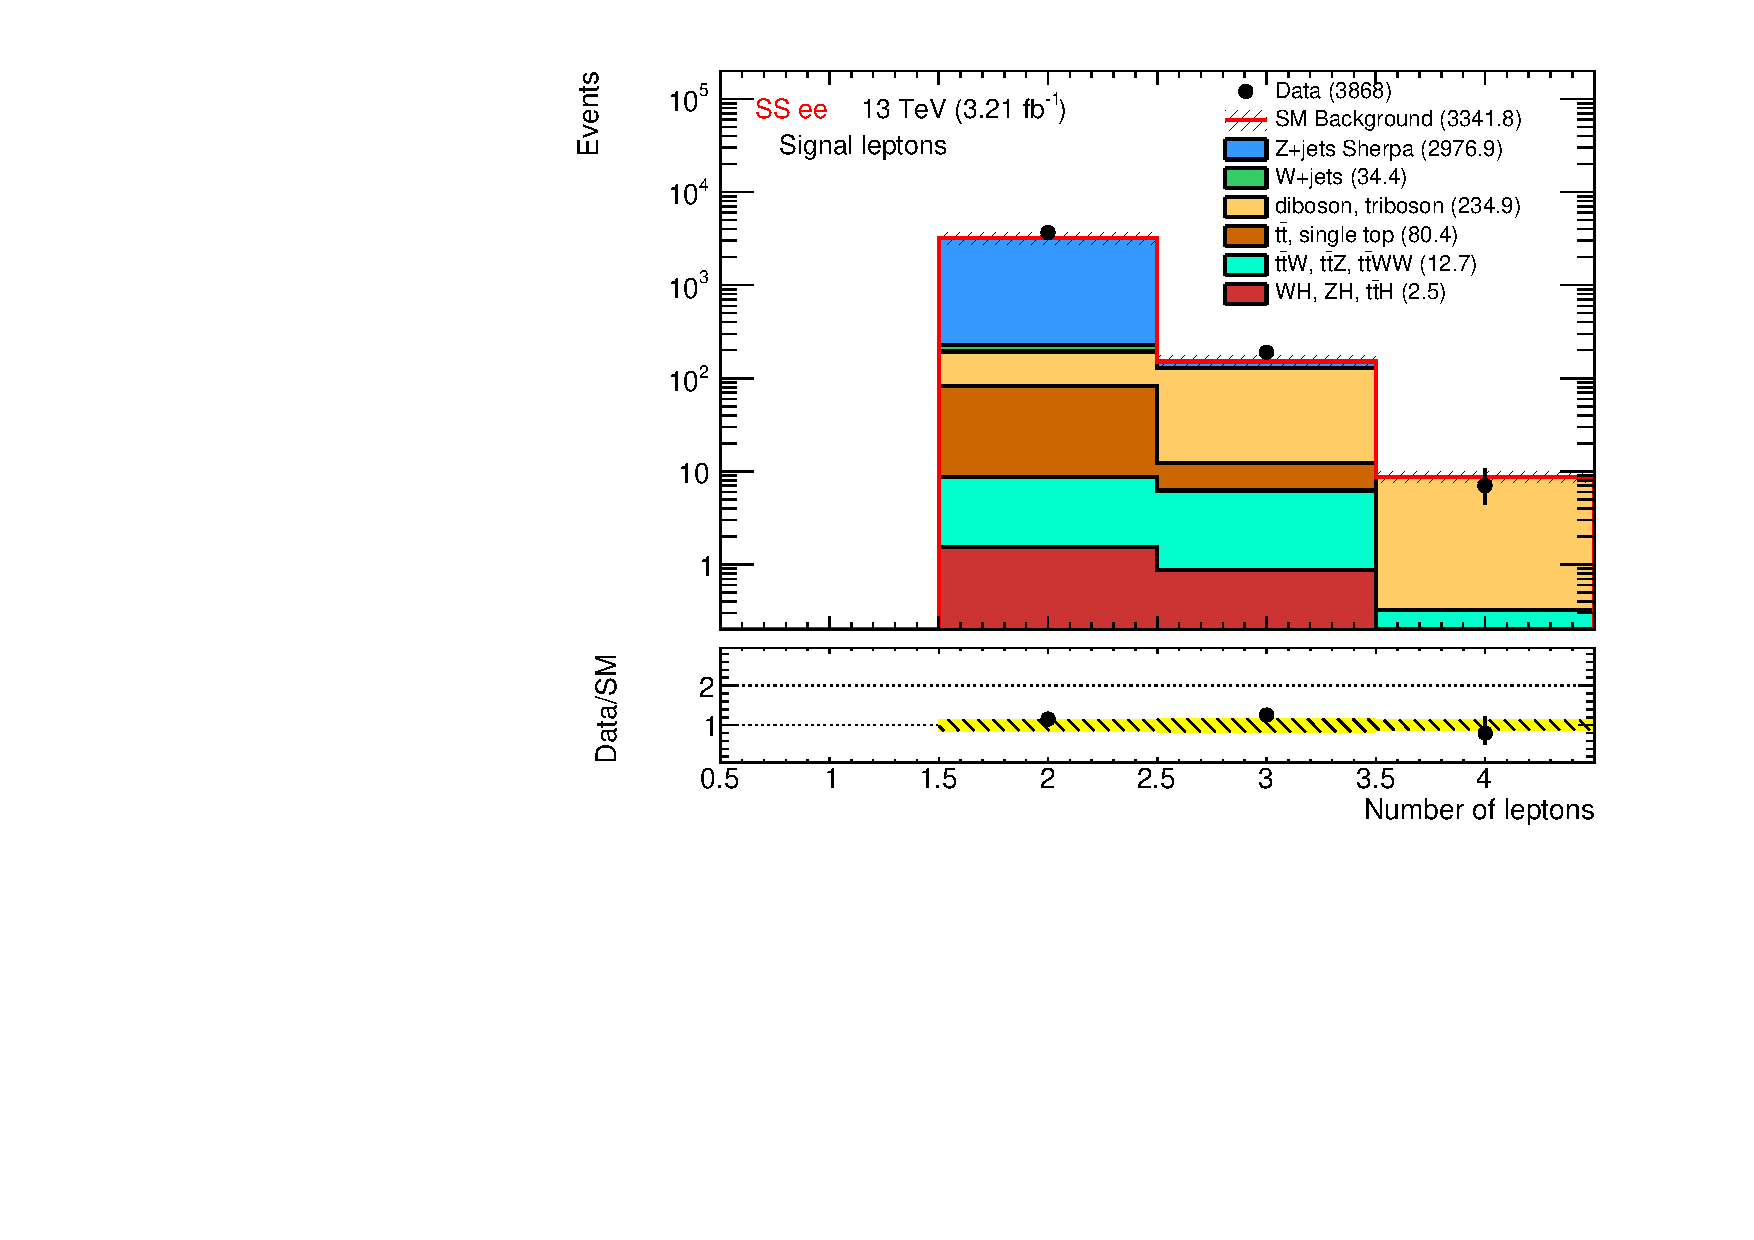
\includegraphics[width=0.49\textwidth]{DATAMC/NLEP_afterlepton_SSee_0_physics.pdf}}
{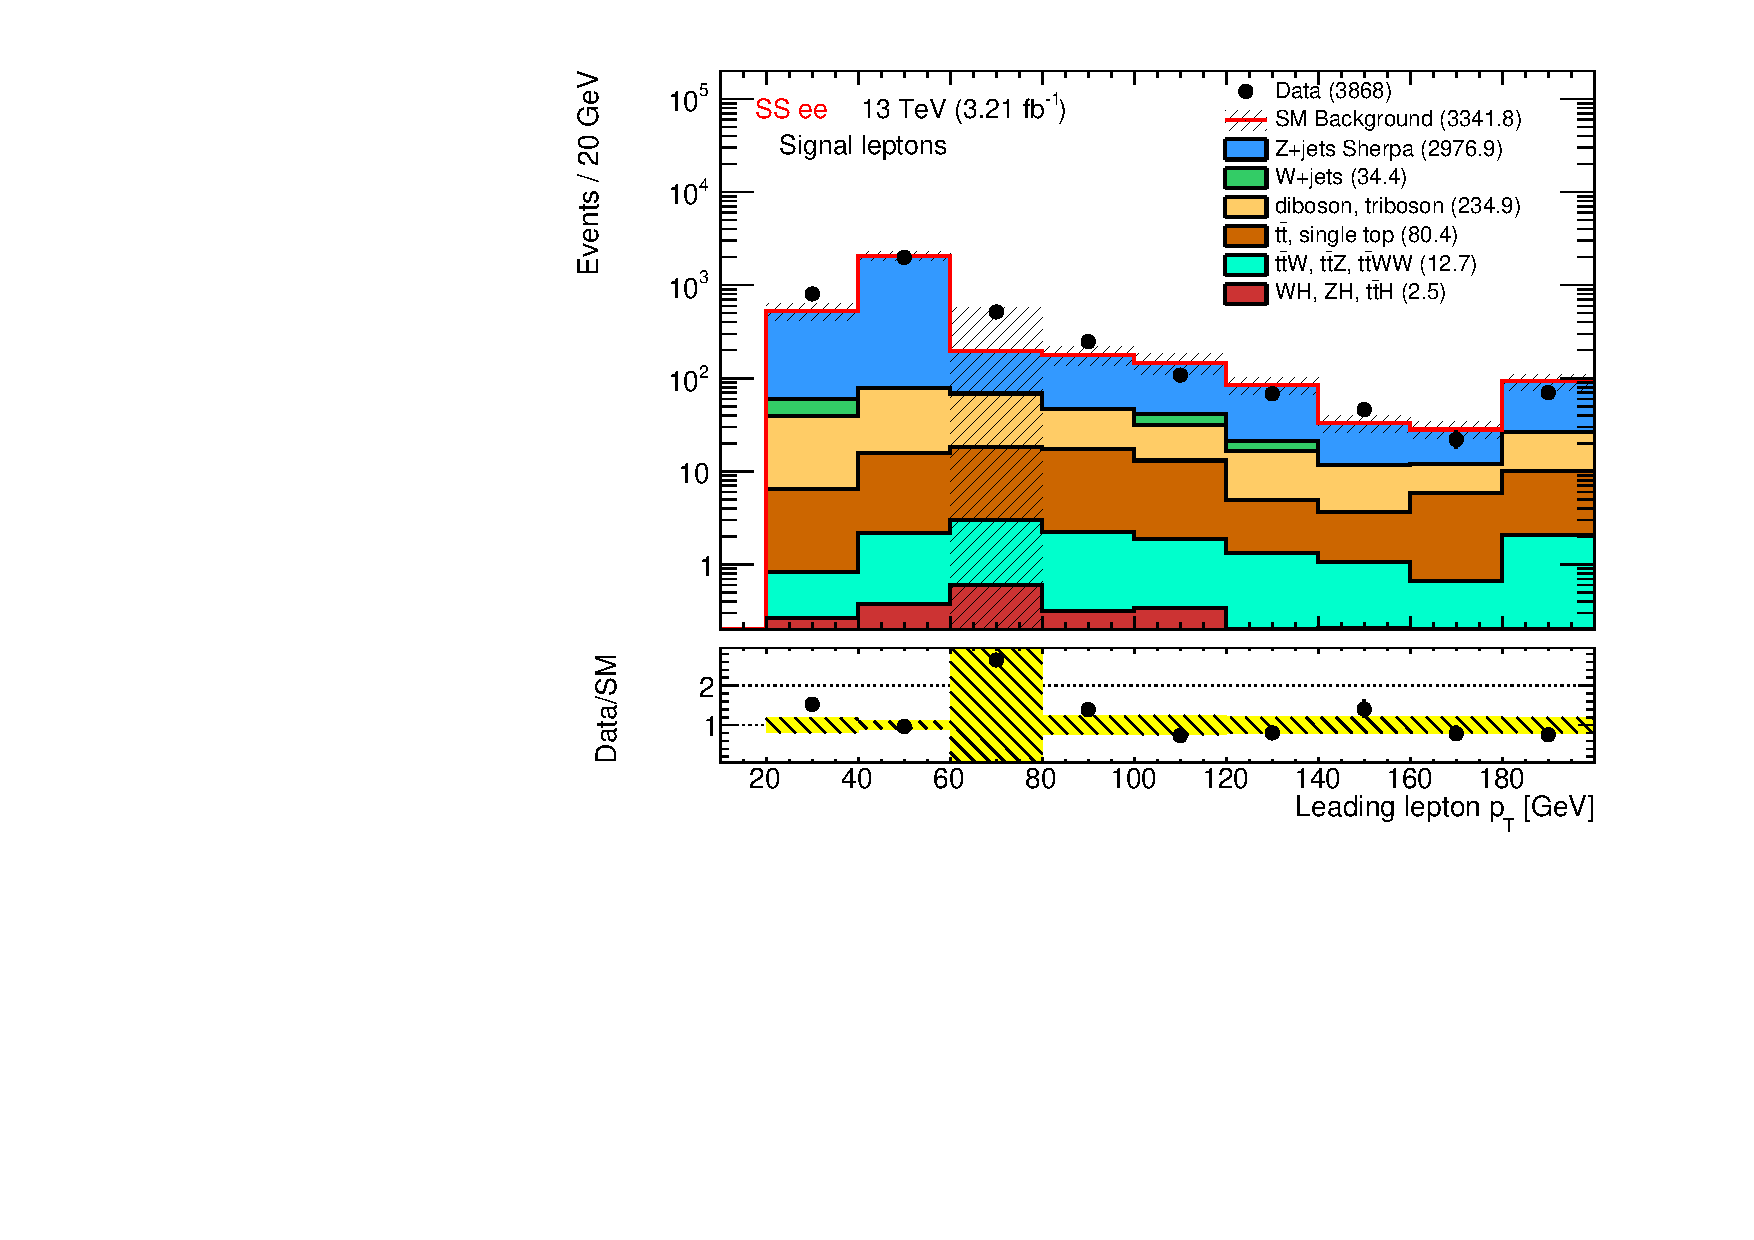
\includegraphics[width=0.49\textwidth]{DATAMC/PTLEP1_afterlepton_SSee_0_physics.pdf}}
{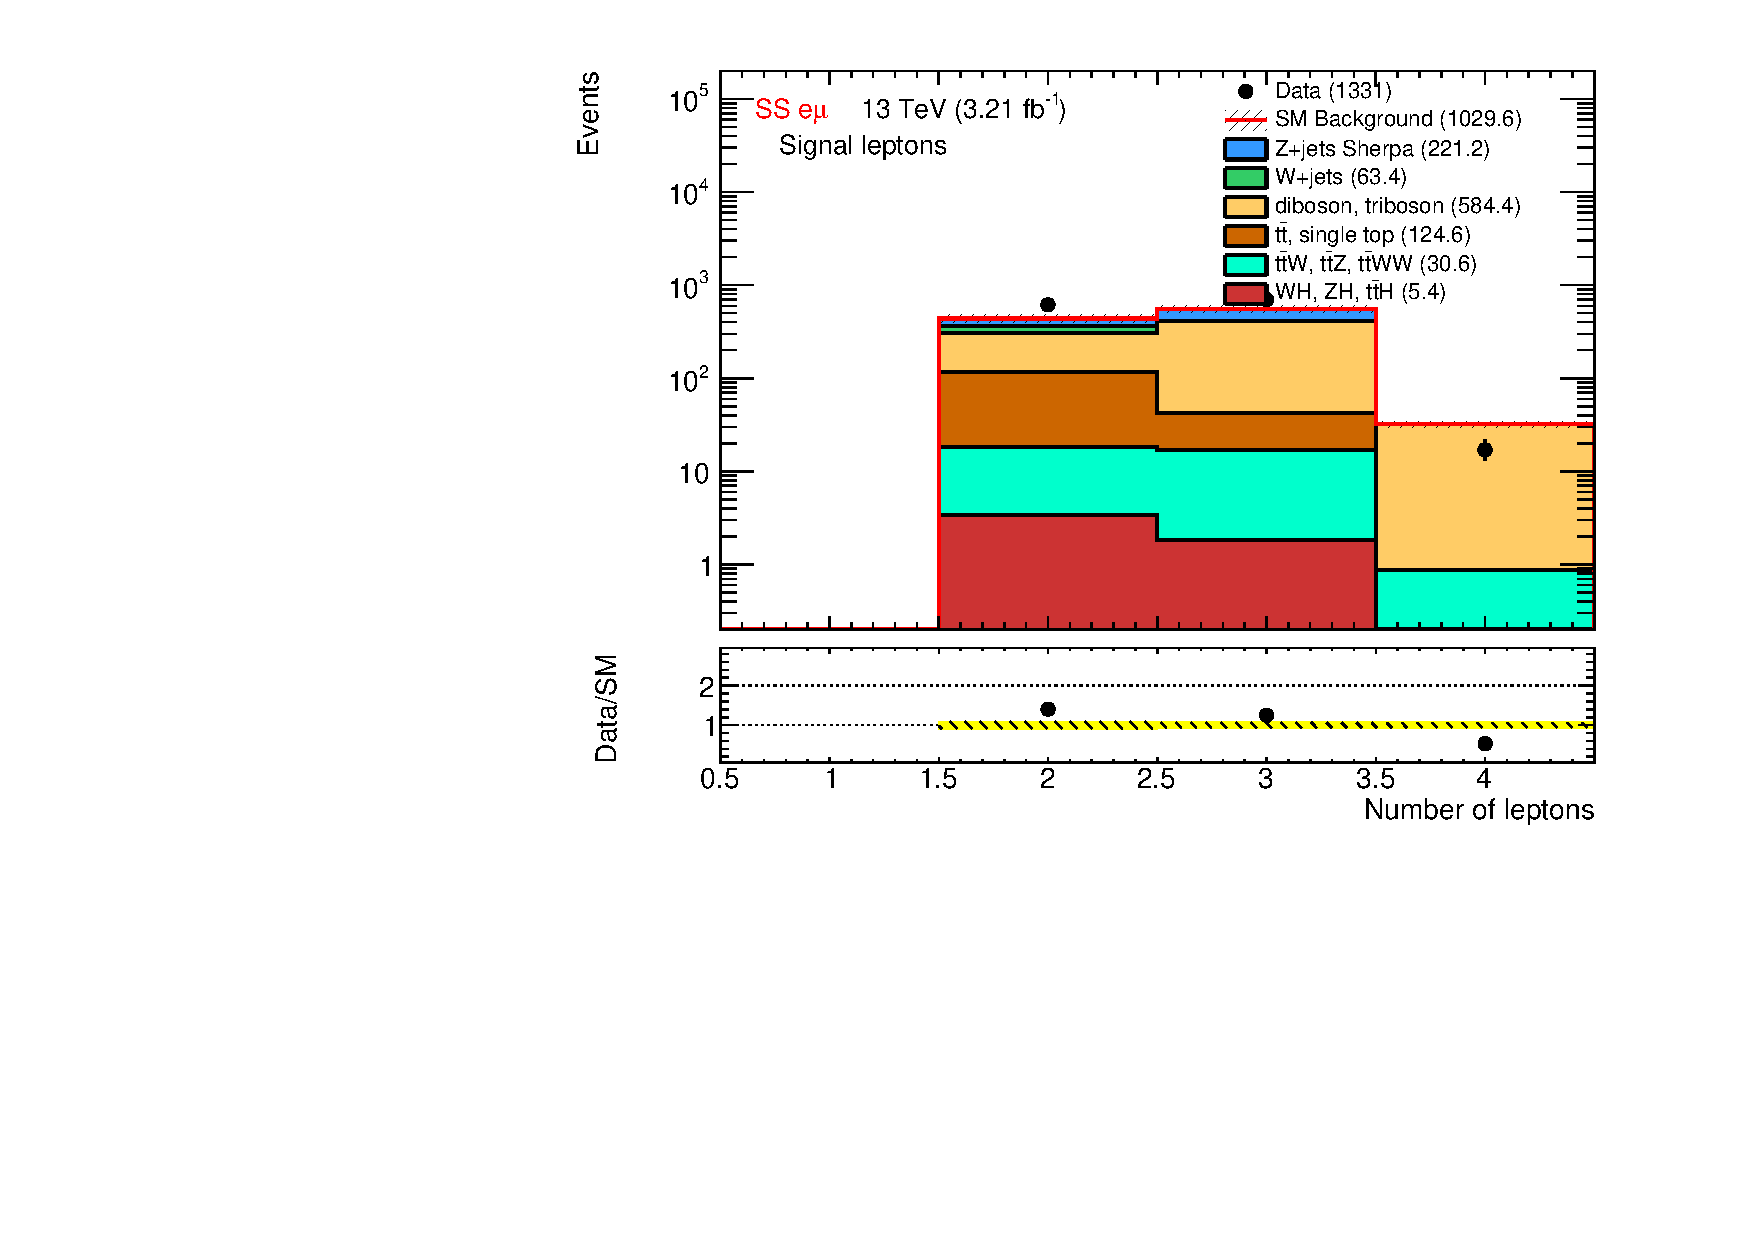
\includegraphics[width=0.49\textwidth]{DATAMC/NLEP_afterlepton_SSem_0_physics.pdf}}
{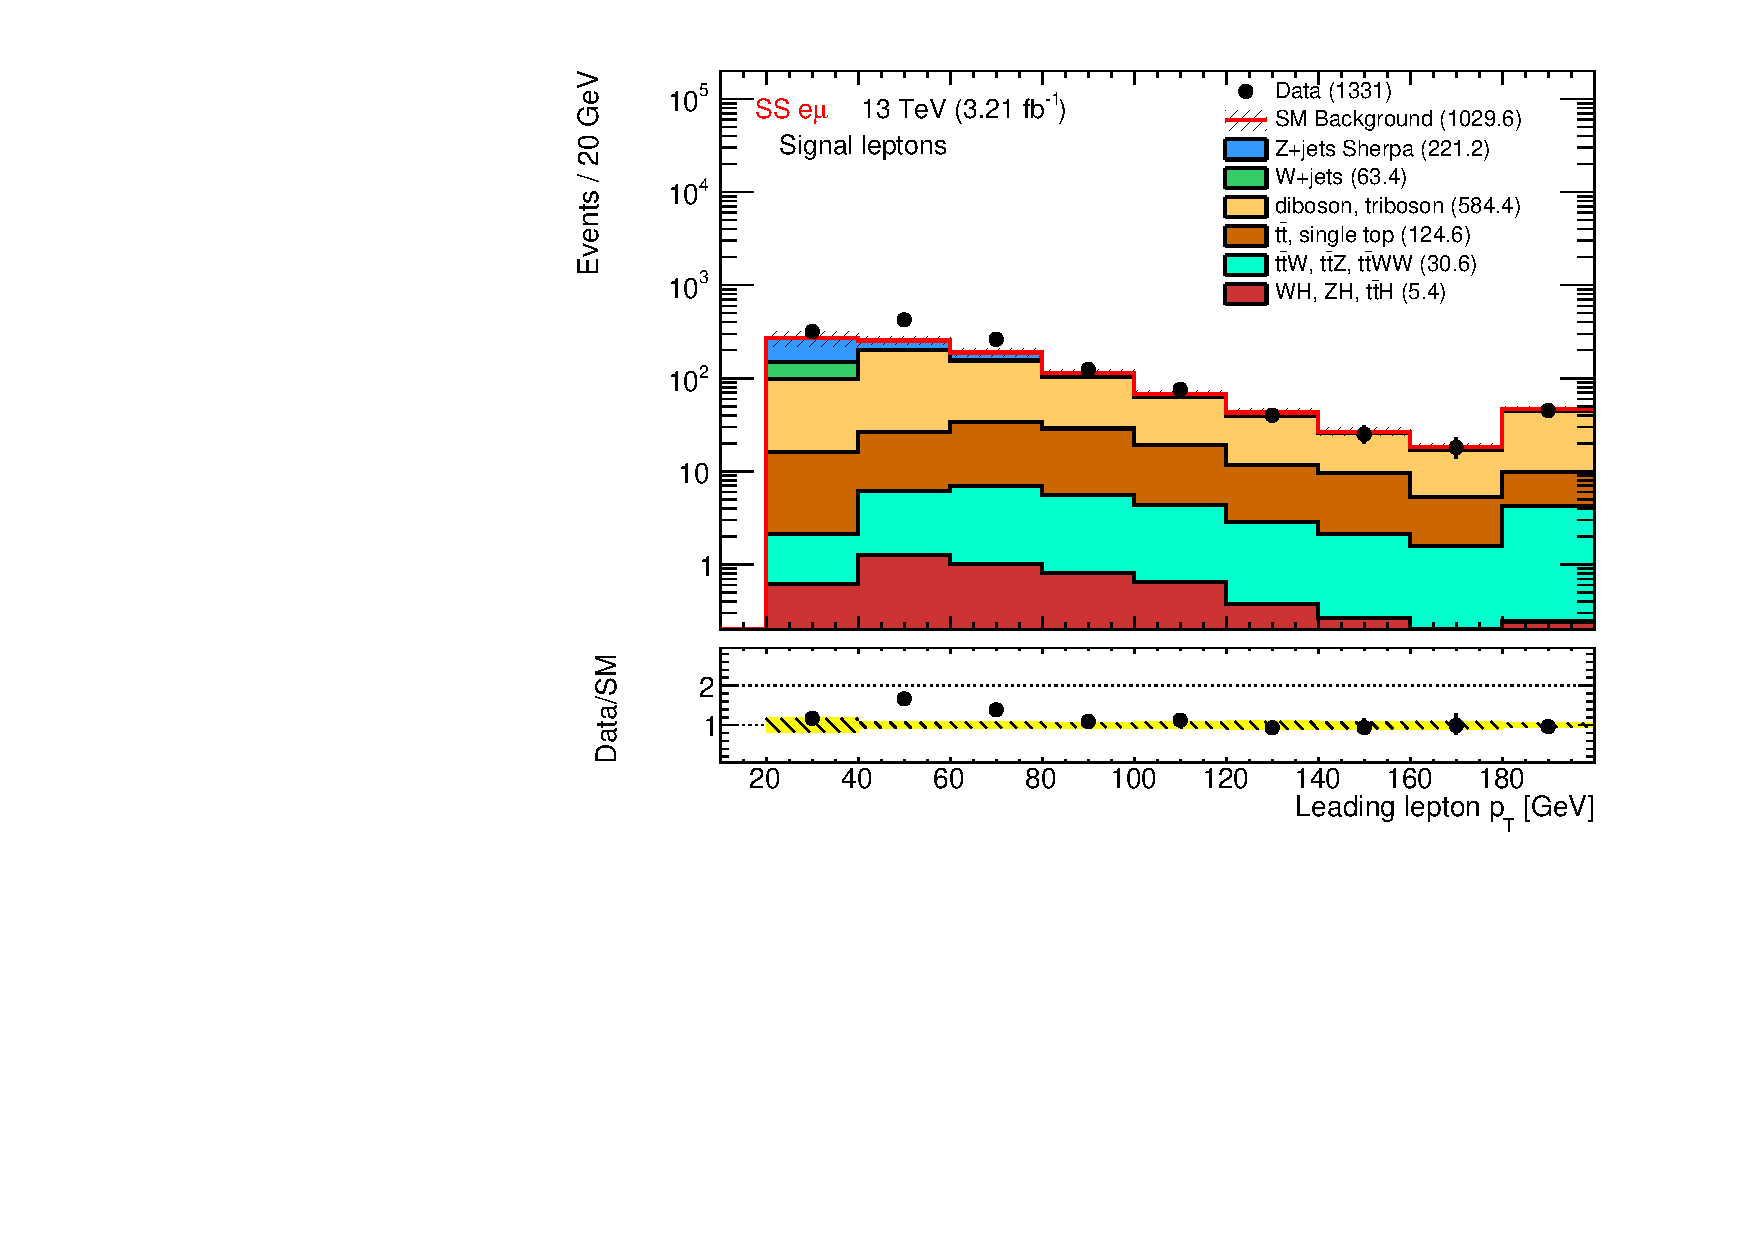
\includegraphics[width=0.49\textwidth]{DATAMC/PTLEP1_afterlepton_SSem_0_physics.pdf}}
{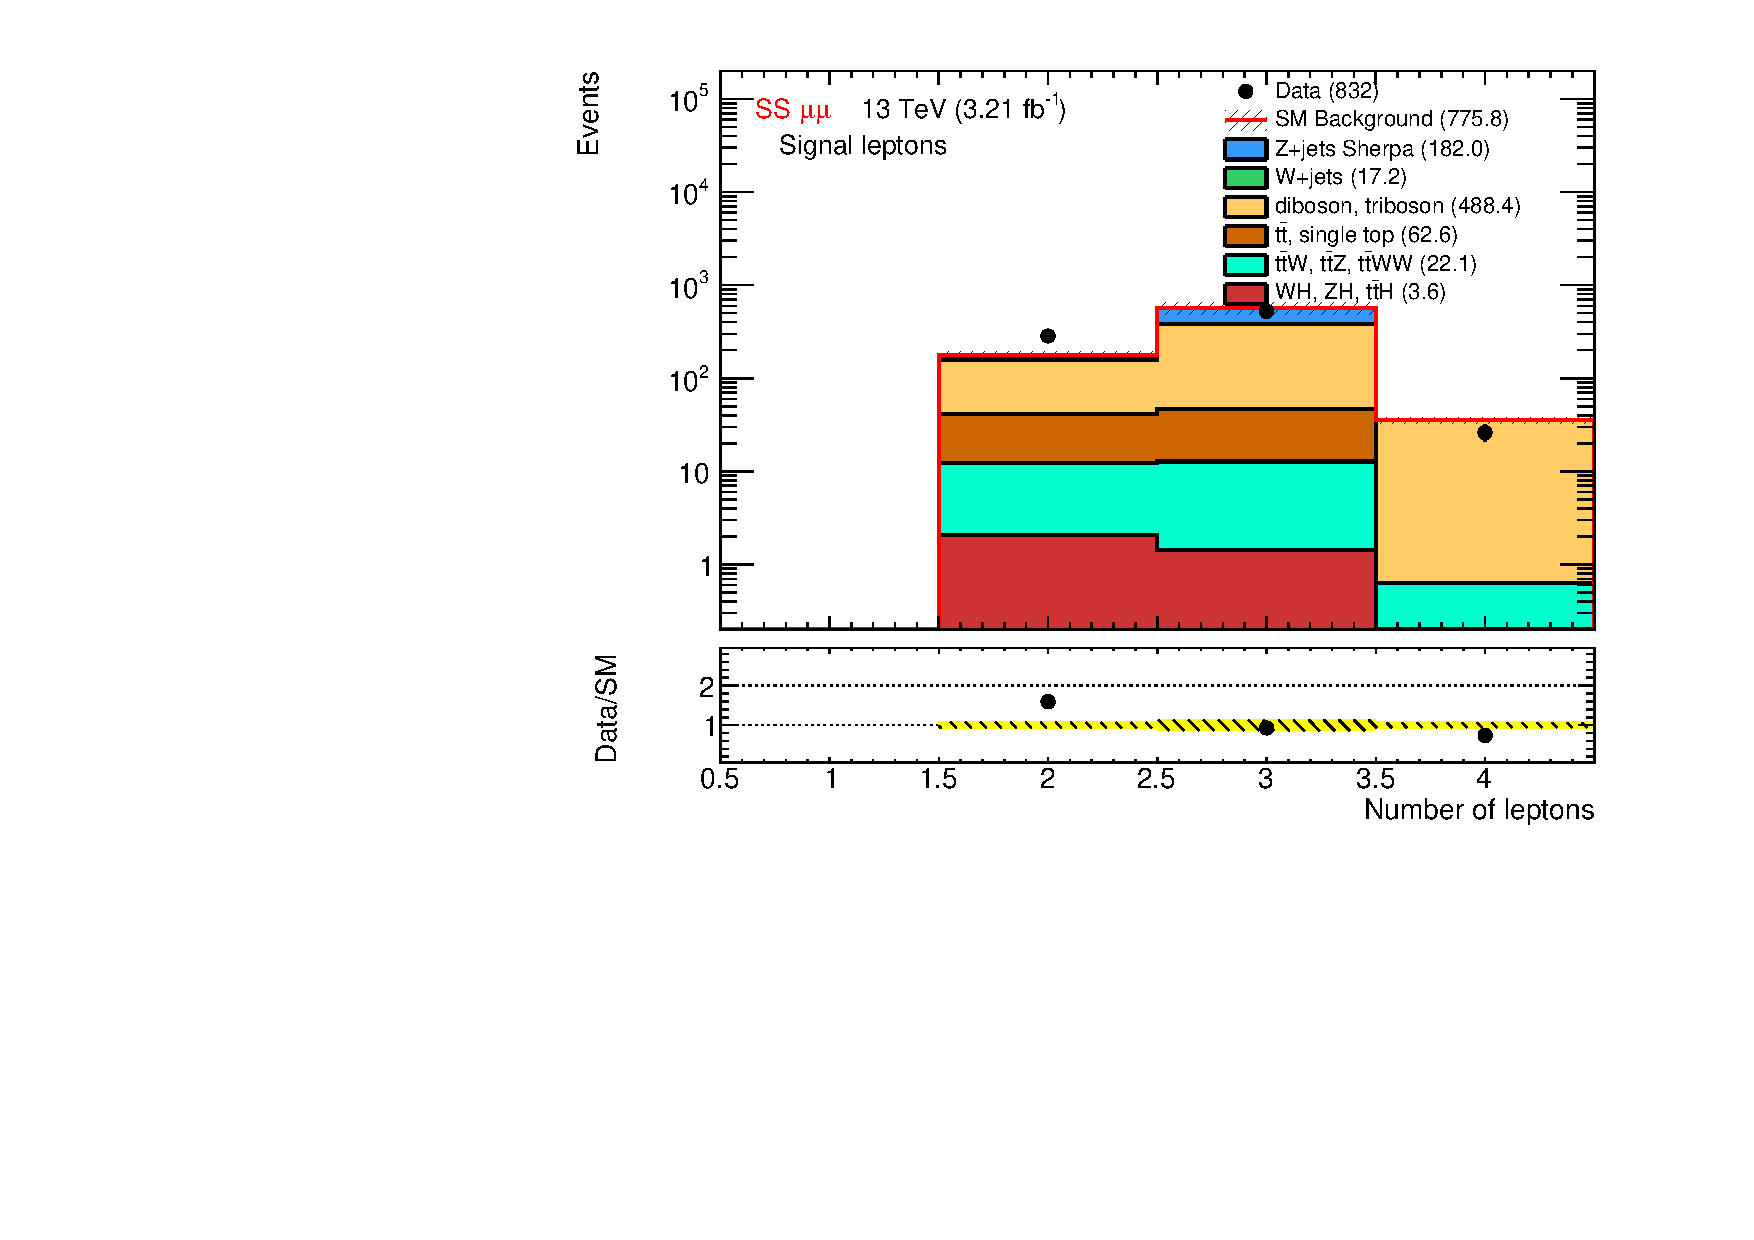
\includegraphics[width=0.49\textwidth]{DATAMC/NLEP_afterlepton_SSmm_0_physics.pdf}}
{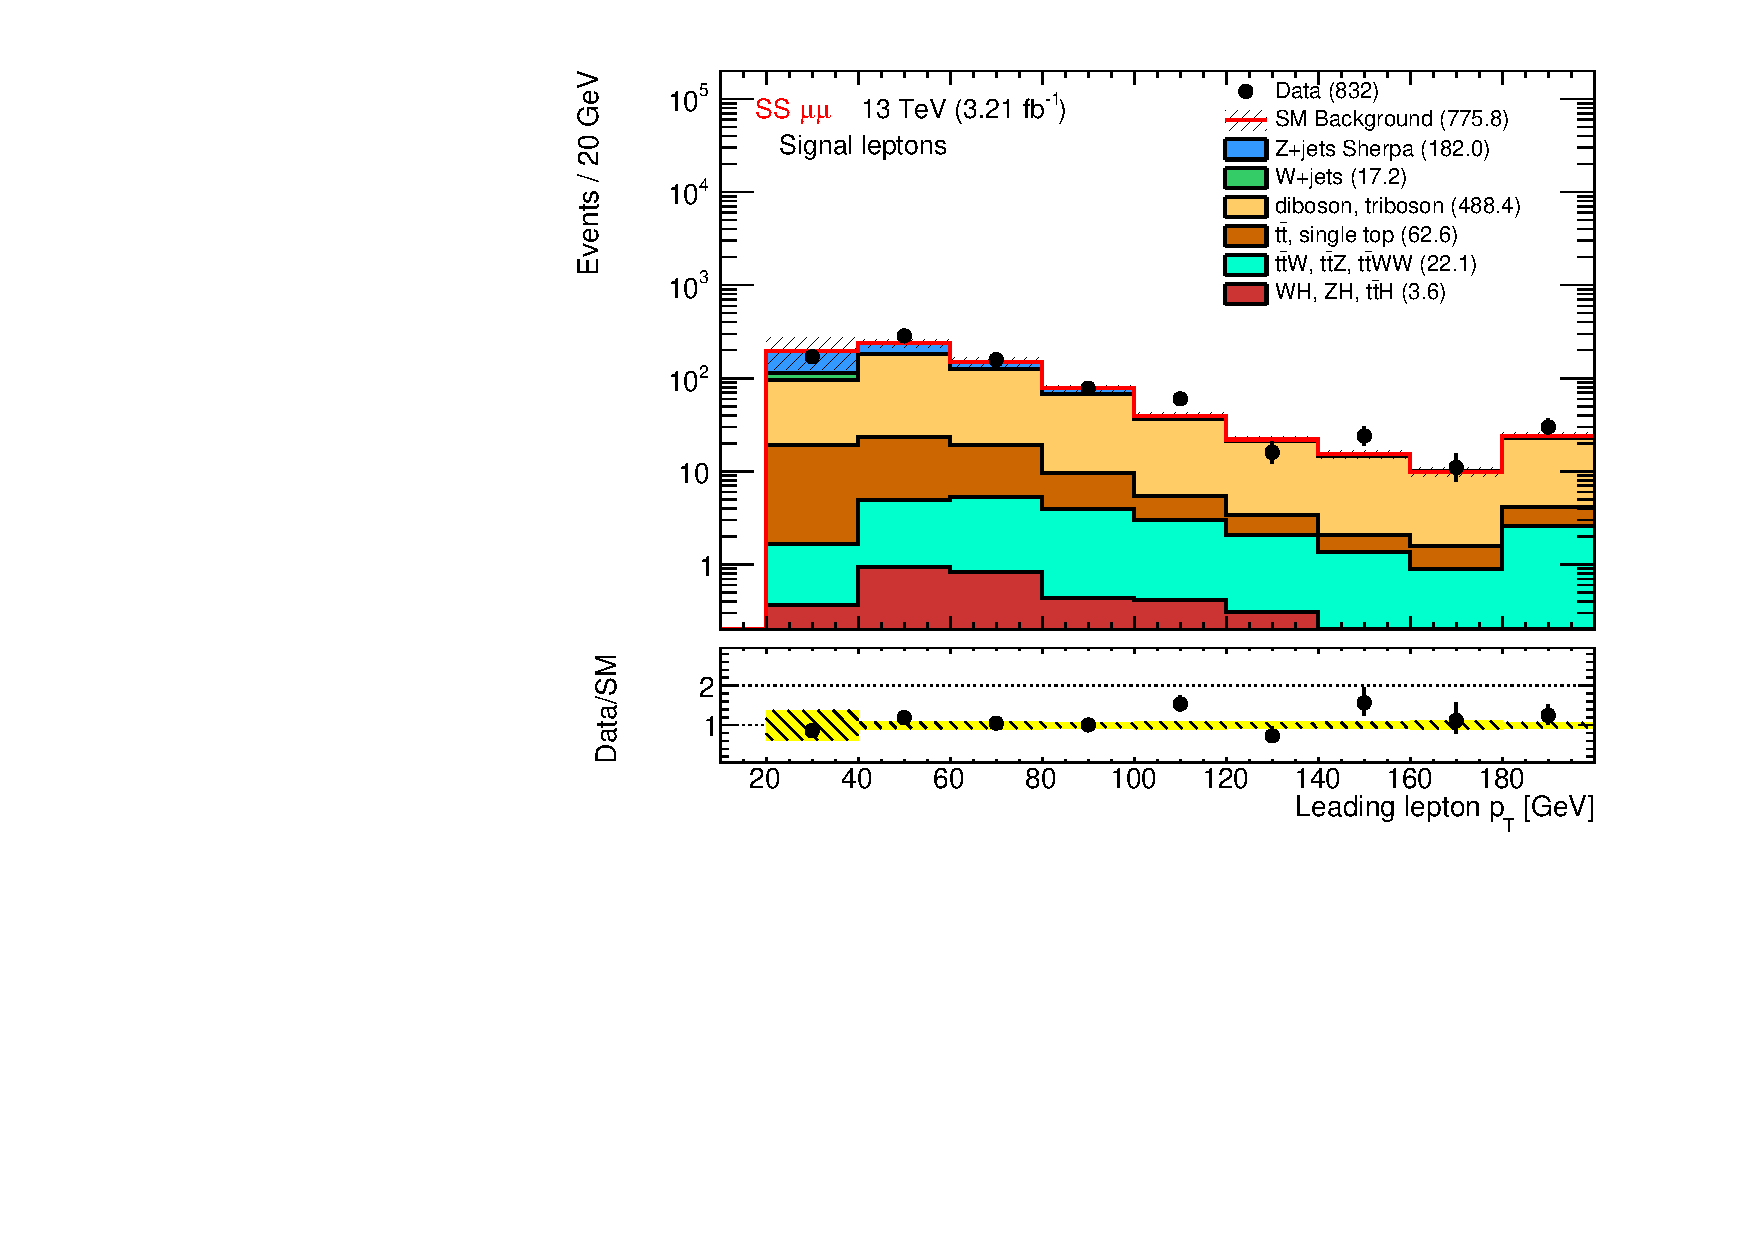
\includegraphics[width=0.49\textwidth]{DATAMC/PTLEP1_afterlepton_SSmm_0_physics.pdf}}
\caption{Lepton multiplicity (left) and leading lepton $\pt$ (right) for events selected in the $ee$ (top), $e\mu$ (center) and $\mu\mu$ (bottom) channels. The background contribution is taken directly from MC with no data-driven estimation of the background with fake and non-prompt leptons or charge mis-identification. Only luminosity and MC statistical uncertainties are included.
}
\label{fig:dataMC_lep1}
\end{figure}

\begin{figure}[htb!]
\centering
{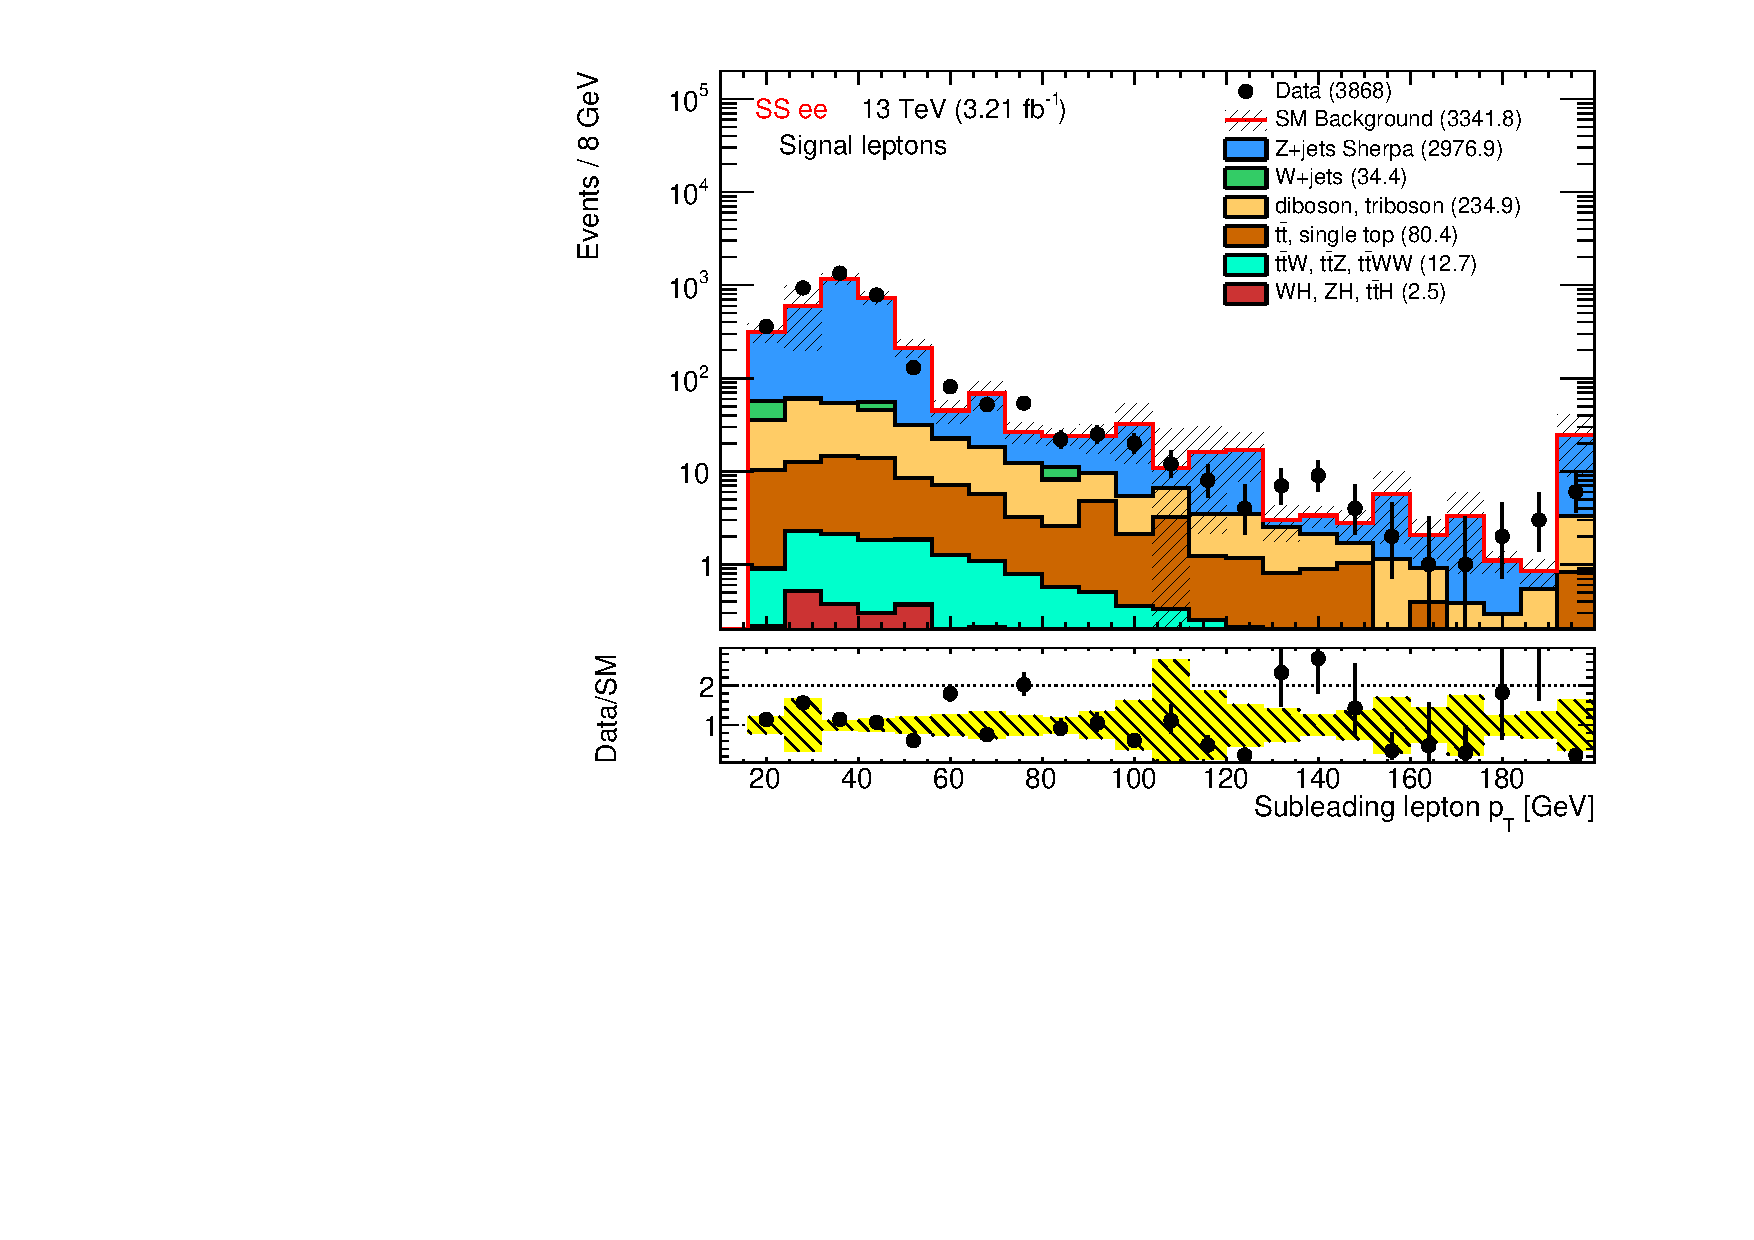
\includegraphics[width=0.49\textwidth]{DATAMC/PTLEP2_afterlepton_SSee_0_physics.pdf}}
{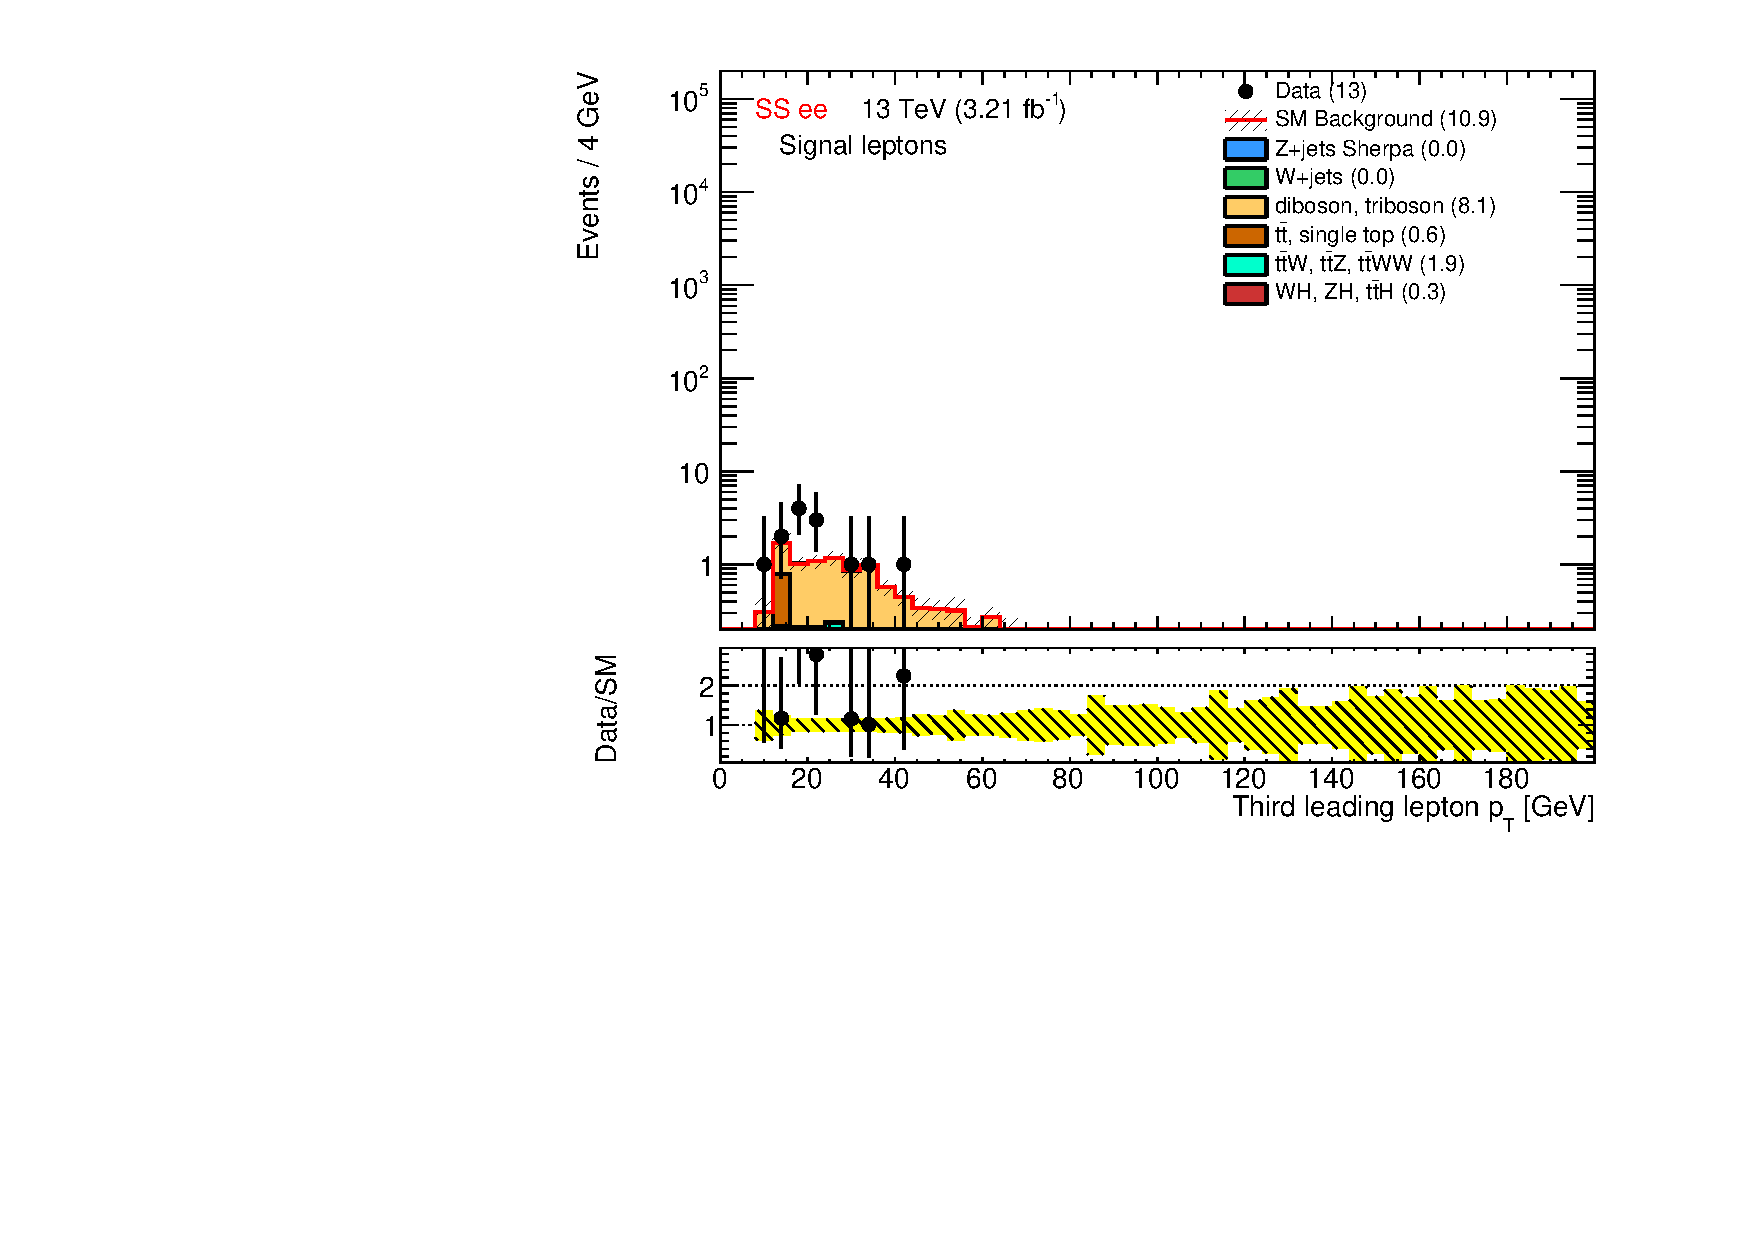
\includegraphics[width=0.49\textwidth]{DATAMC/PTLEP3_afterlepton_SSee_0_physics.pdf}}
{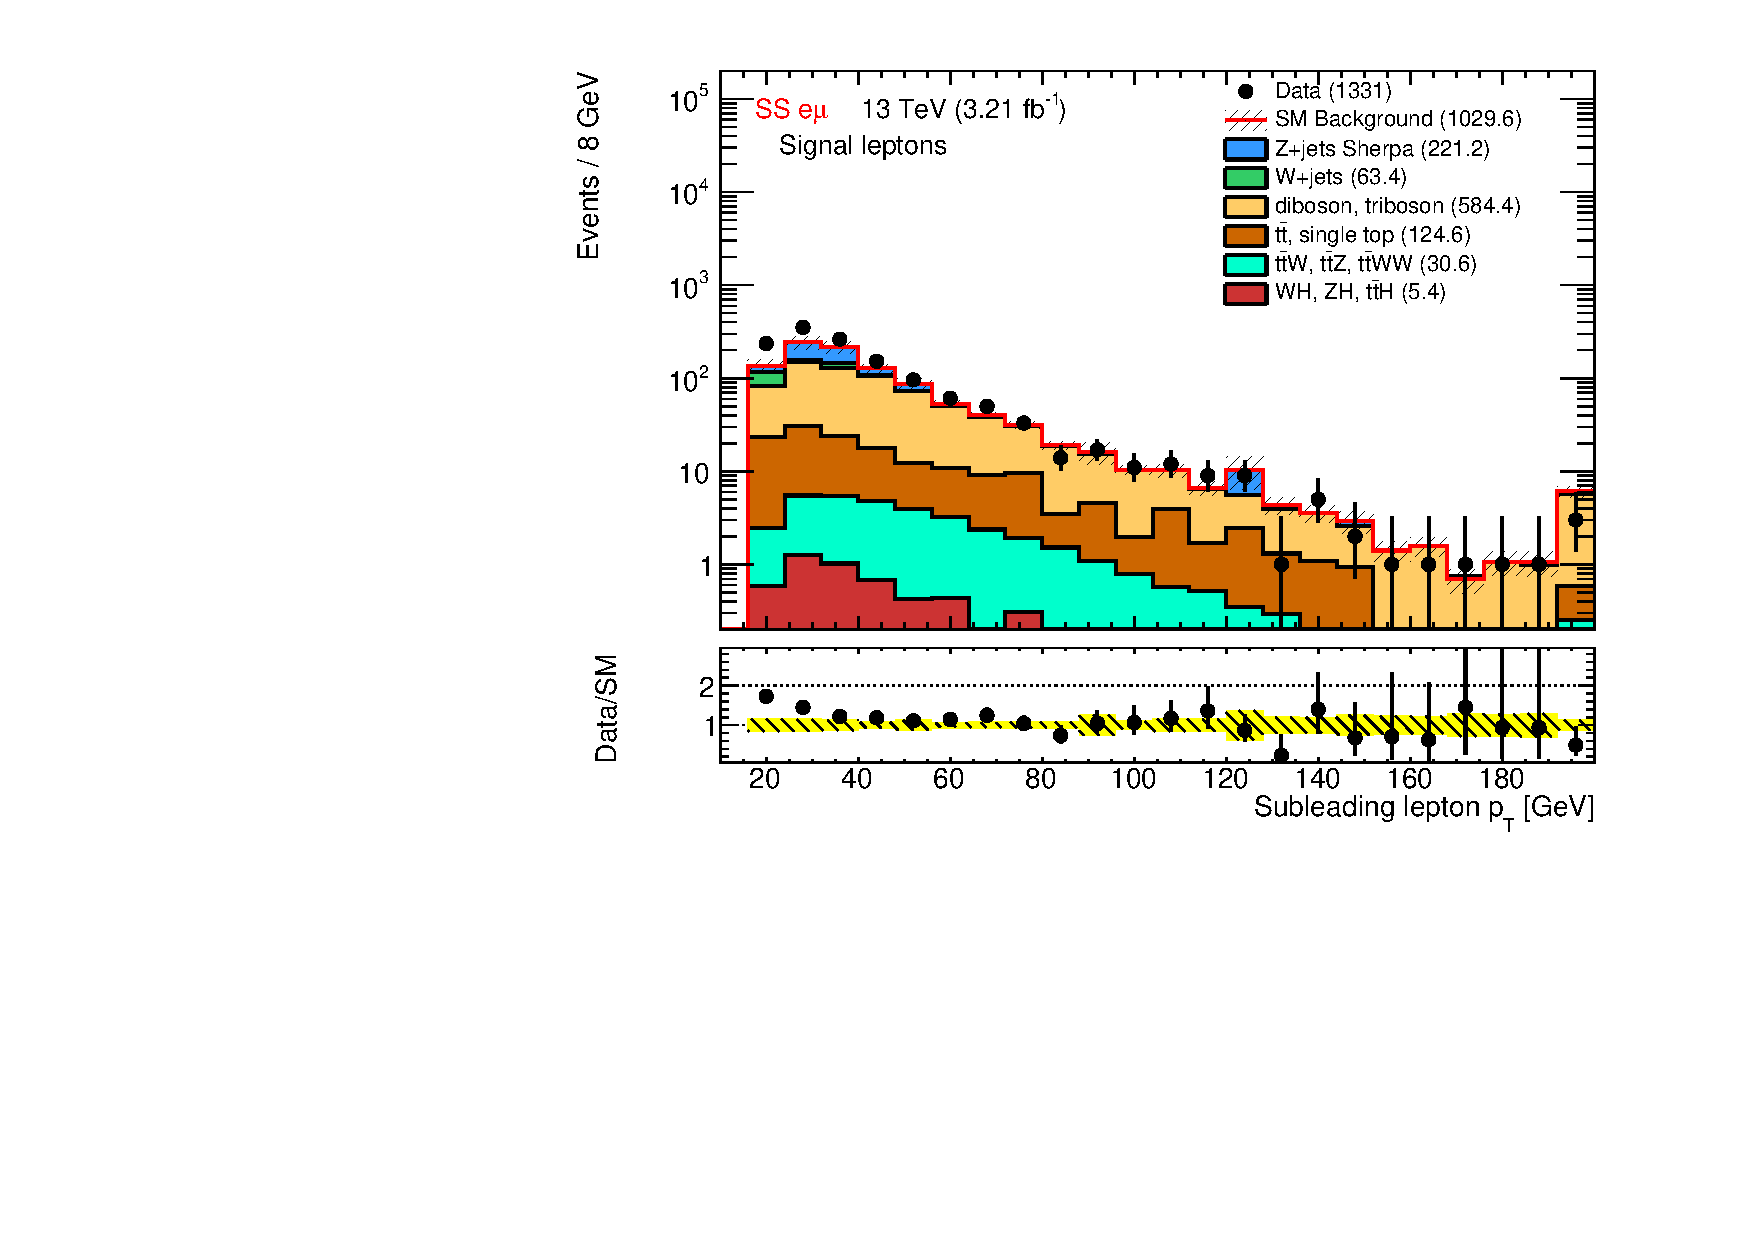
\includegraphics[width=0.49\textwidth]{DATAMC/PTLEP2_afterlepton_SSem_0_physics.pdf}}
{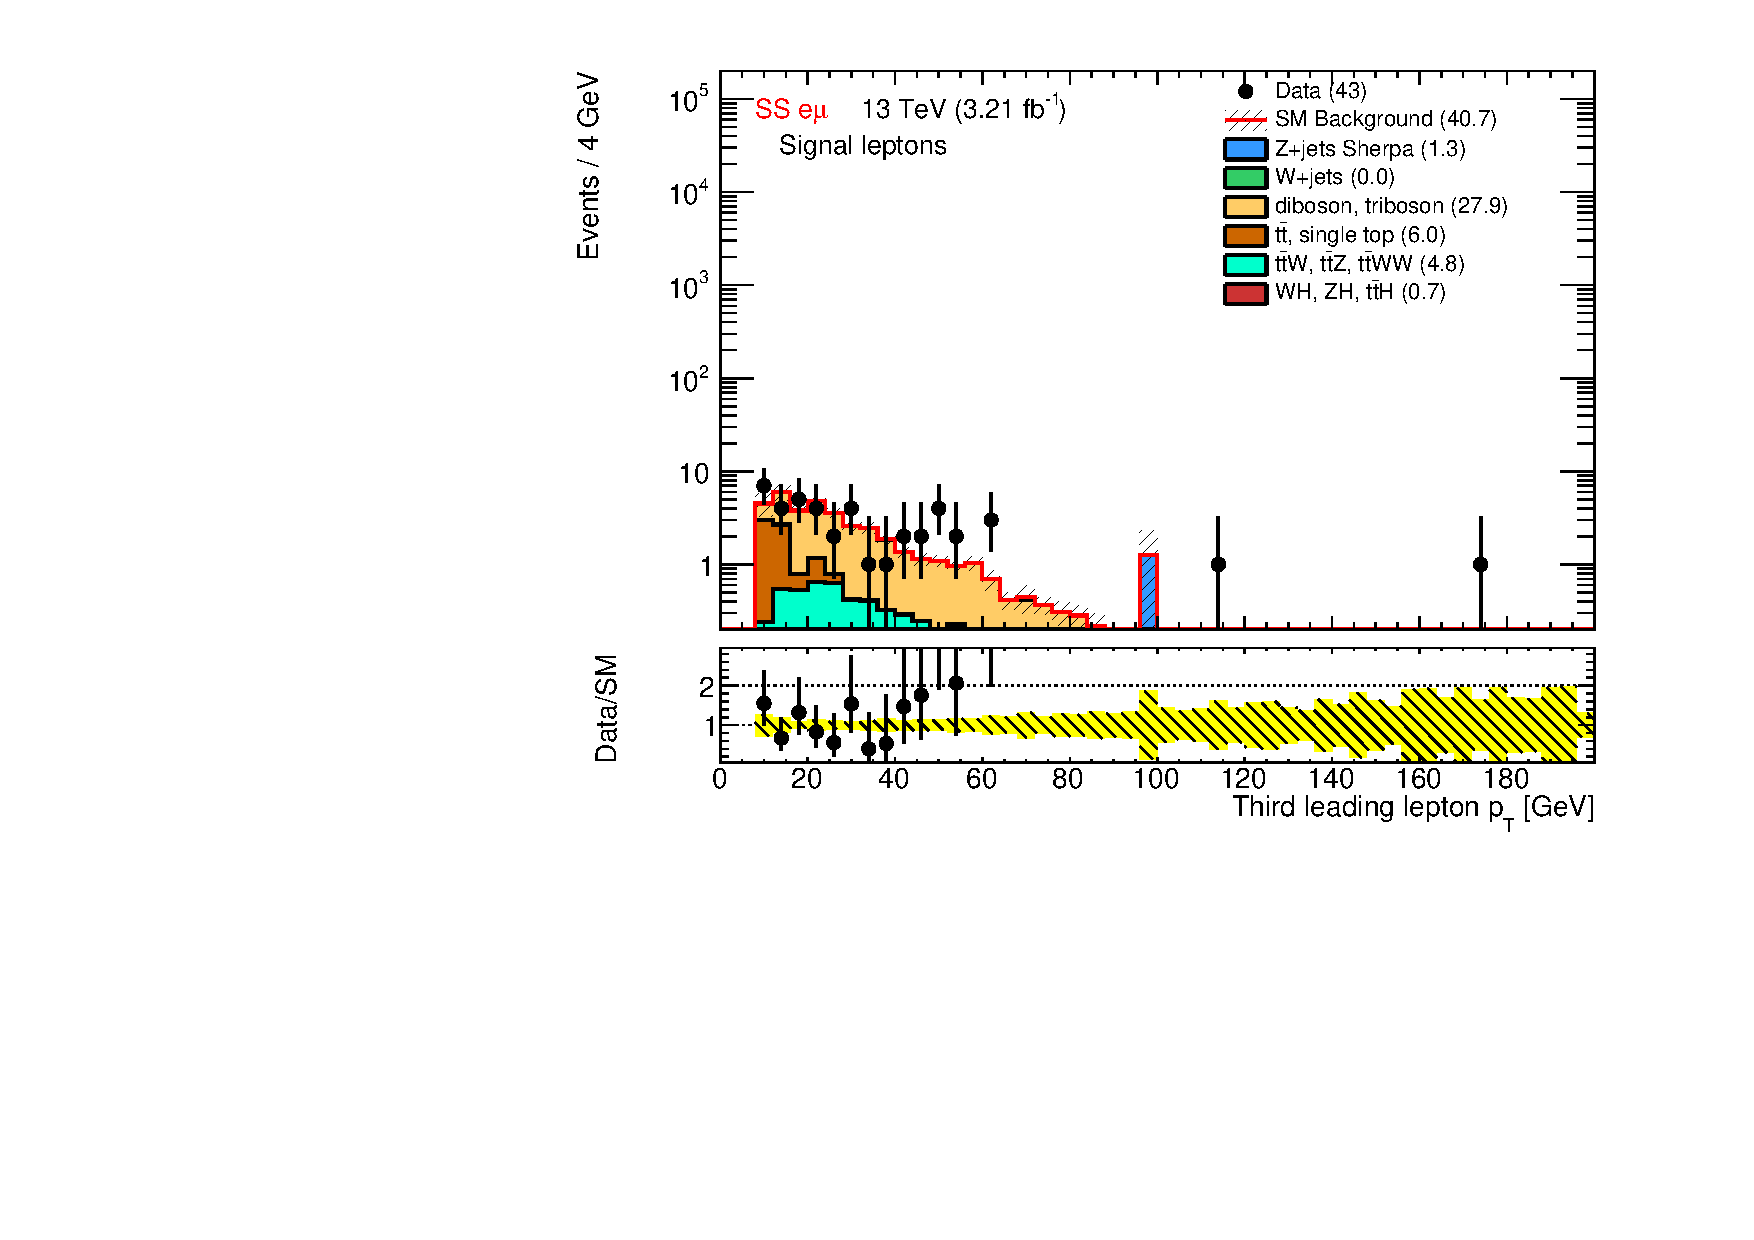
\includegraphics[width=0.49\textwidth]{DATAMC/PTLEP3_afterlepton_SSem_0_physics.pdf}}
{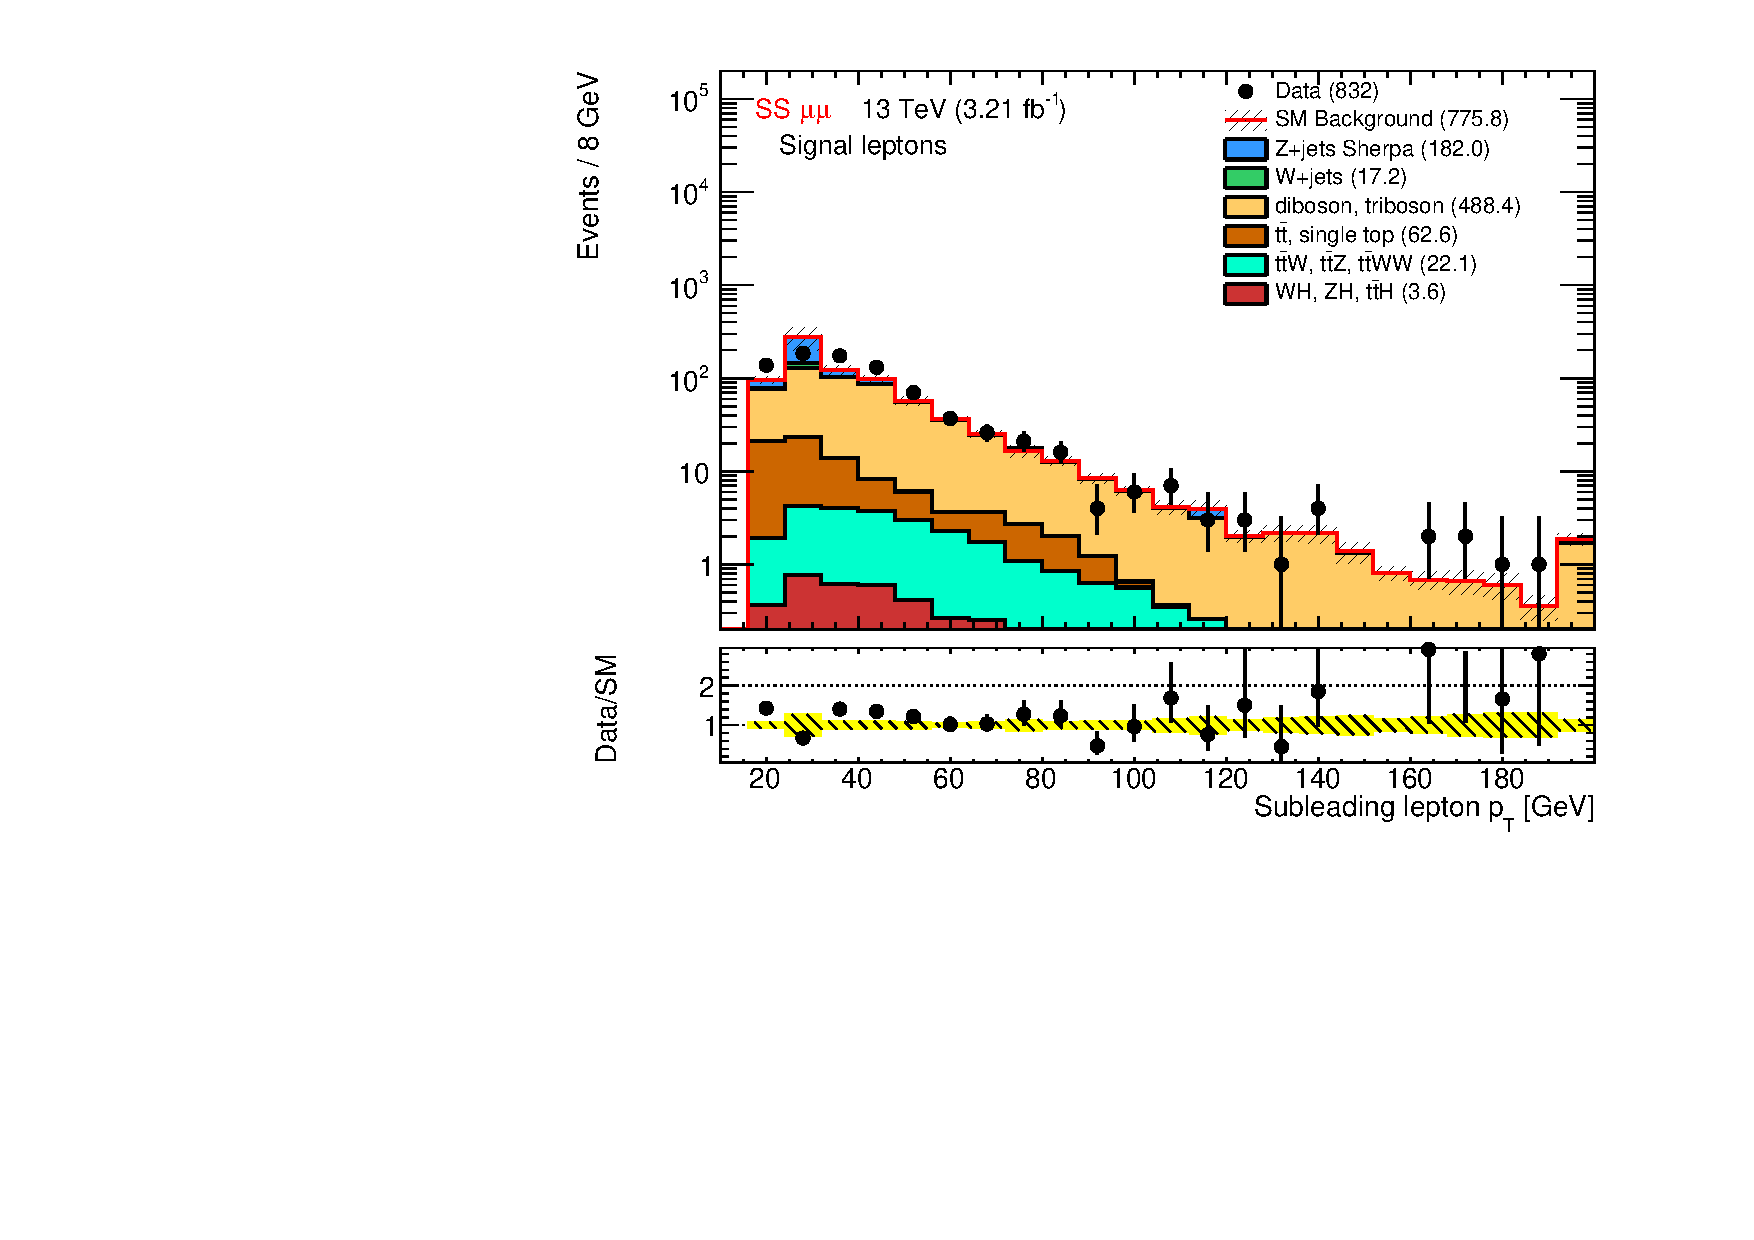
\includegraphics[width=0.49\textwidth]{DATAMC/PTLEP2_afterlepton_SSmm_0_physics.pdf}}
{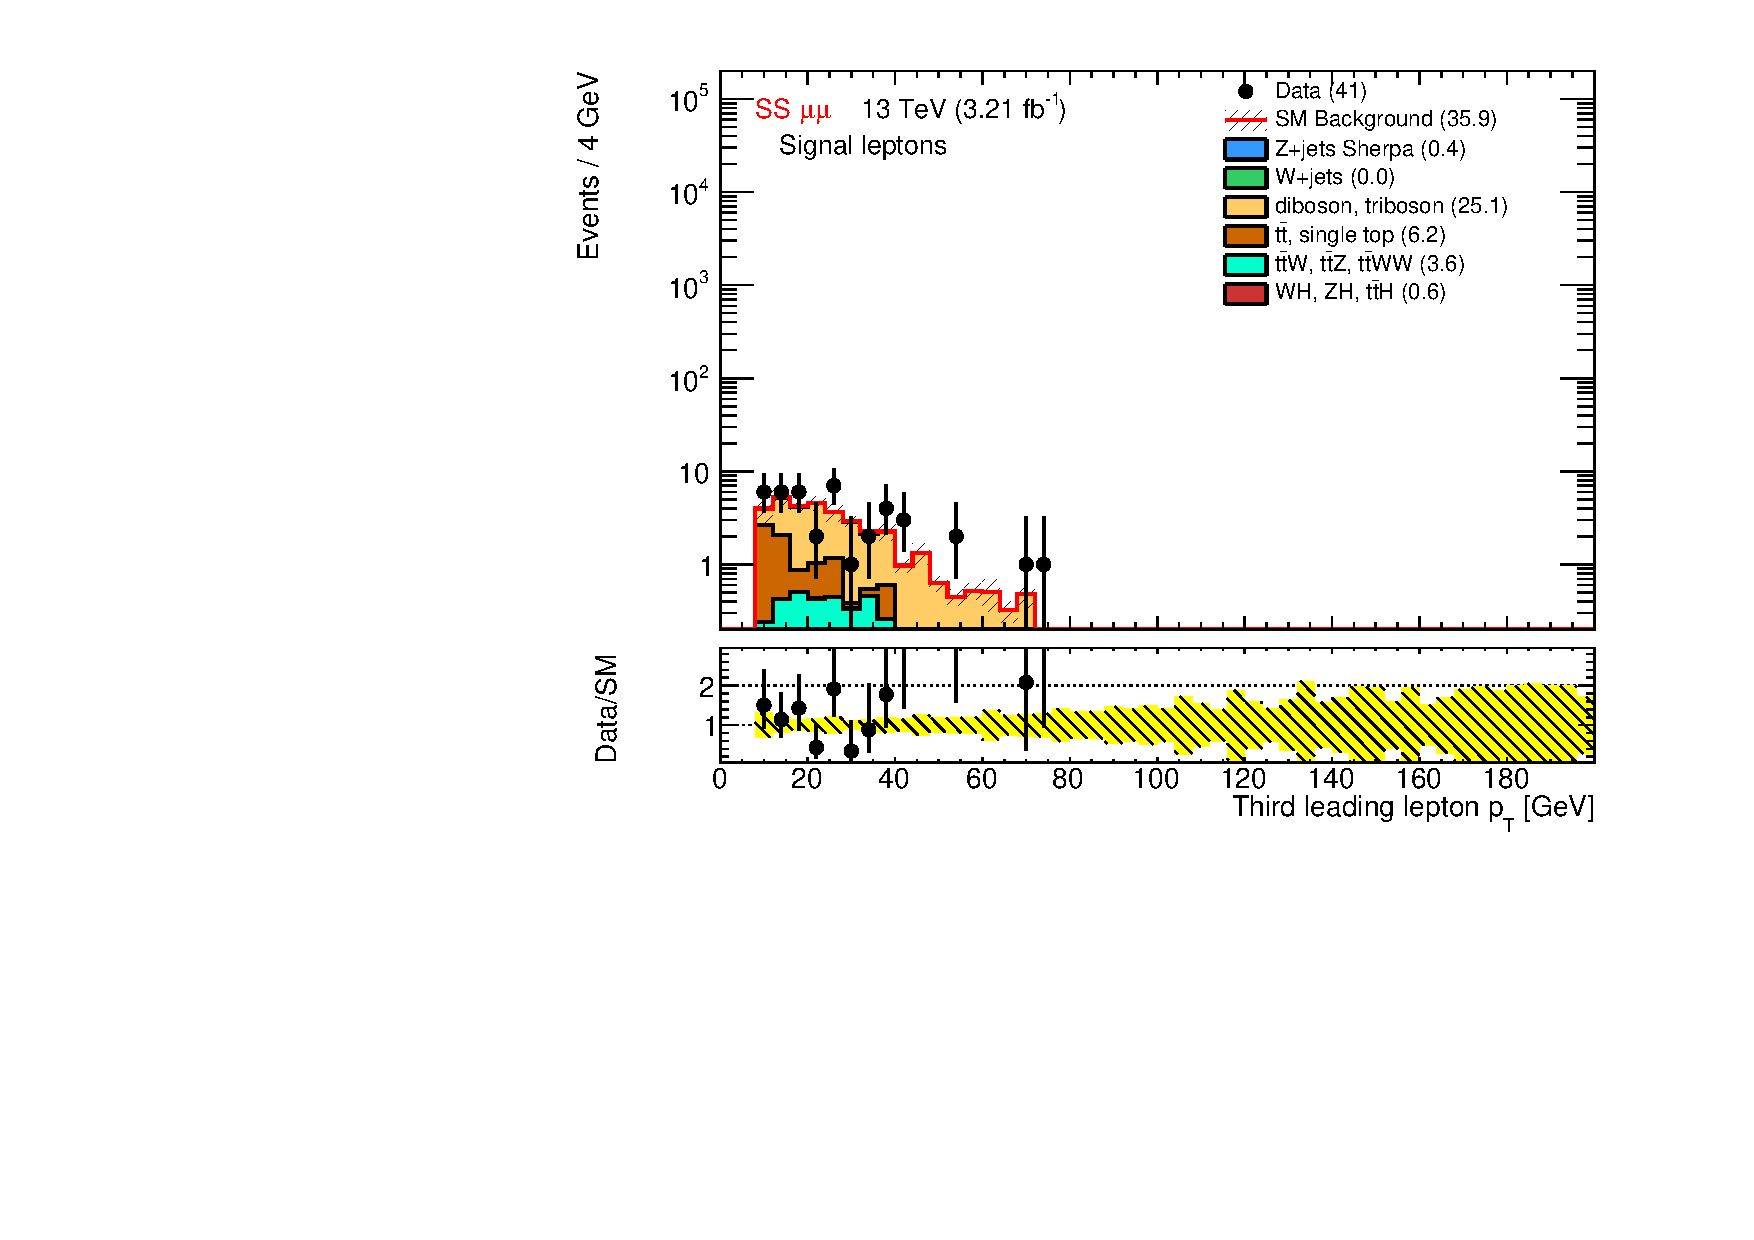
\includegraphics[width=0.49\textwidth]{DATAMC/PTLEP3_afterlepton_SSmm_0_physics.pdf}}
\caption{Sub-leading (left) and third leading lepton $\pt$ (right) for events selected in the $ee$ (top), $e\mu$ (center) and $\mu\mu$ (bottom) channels. The background contribution is taken directly from MC with no data-driven estimation of the background with fake and non-prompt leptons or charge mis-identification. Only luminosity and MC statistical uncertainties are included.
}
\label{fig:dataMC_lep2}
\end{figure}


\begin{figure}[htb!]
\centering
{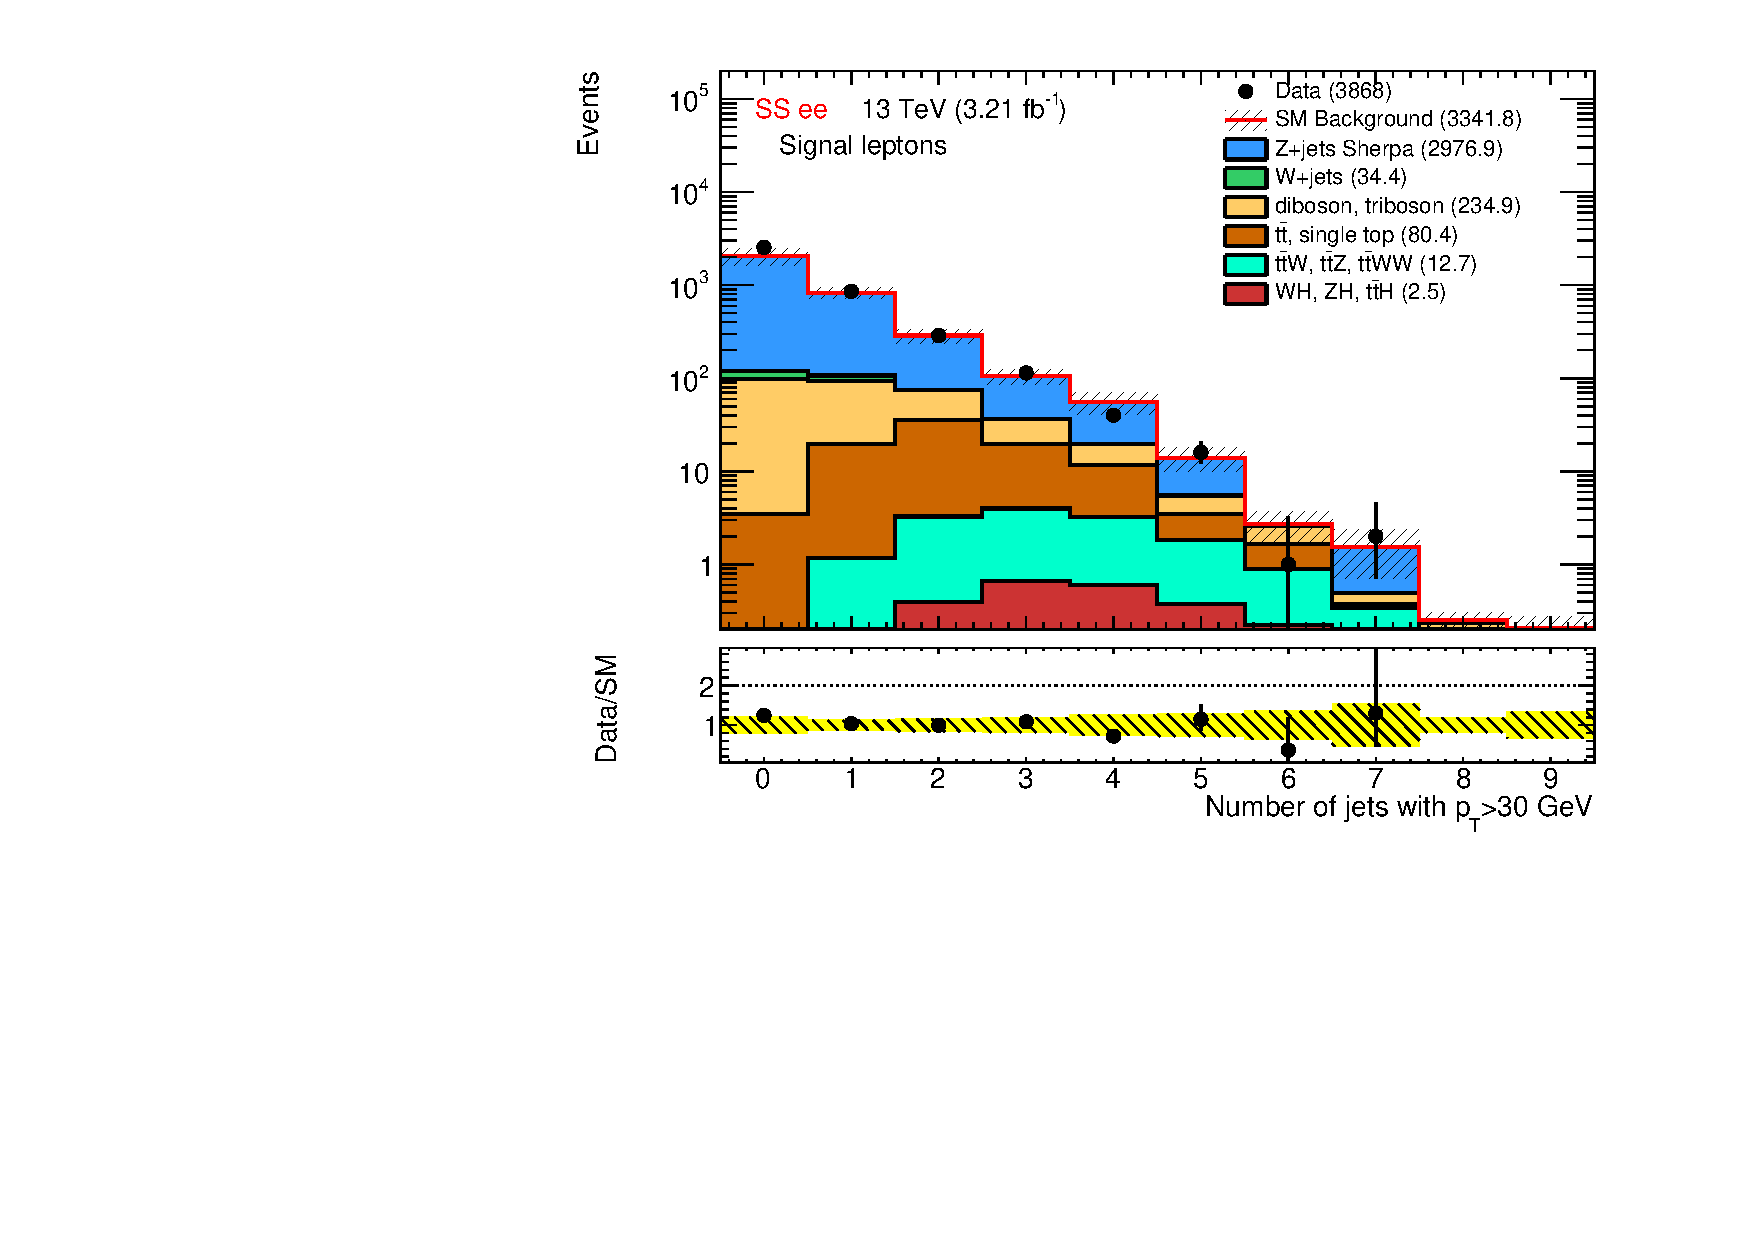
\includegraphics[width=0.49\textwidth]{DATAMC/NJET30_afterlepton_SSee_0_physics.pdf}}
{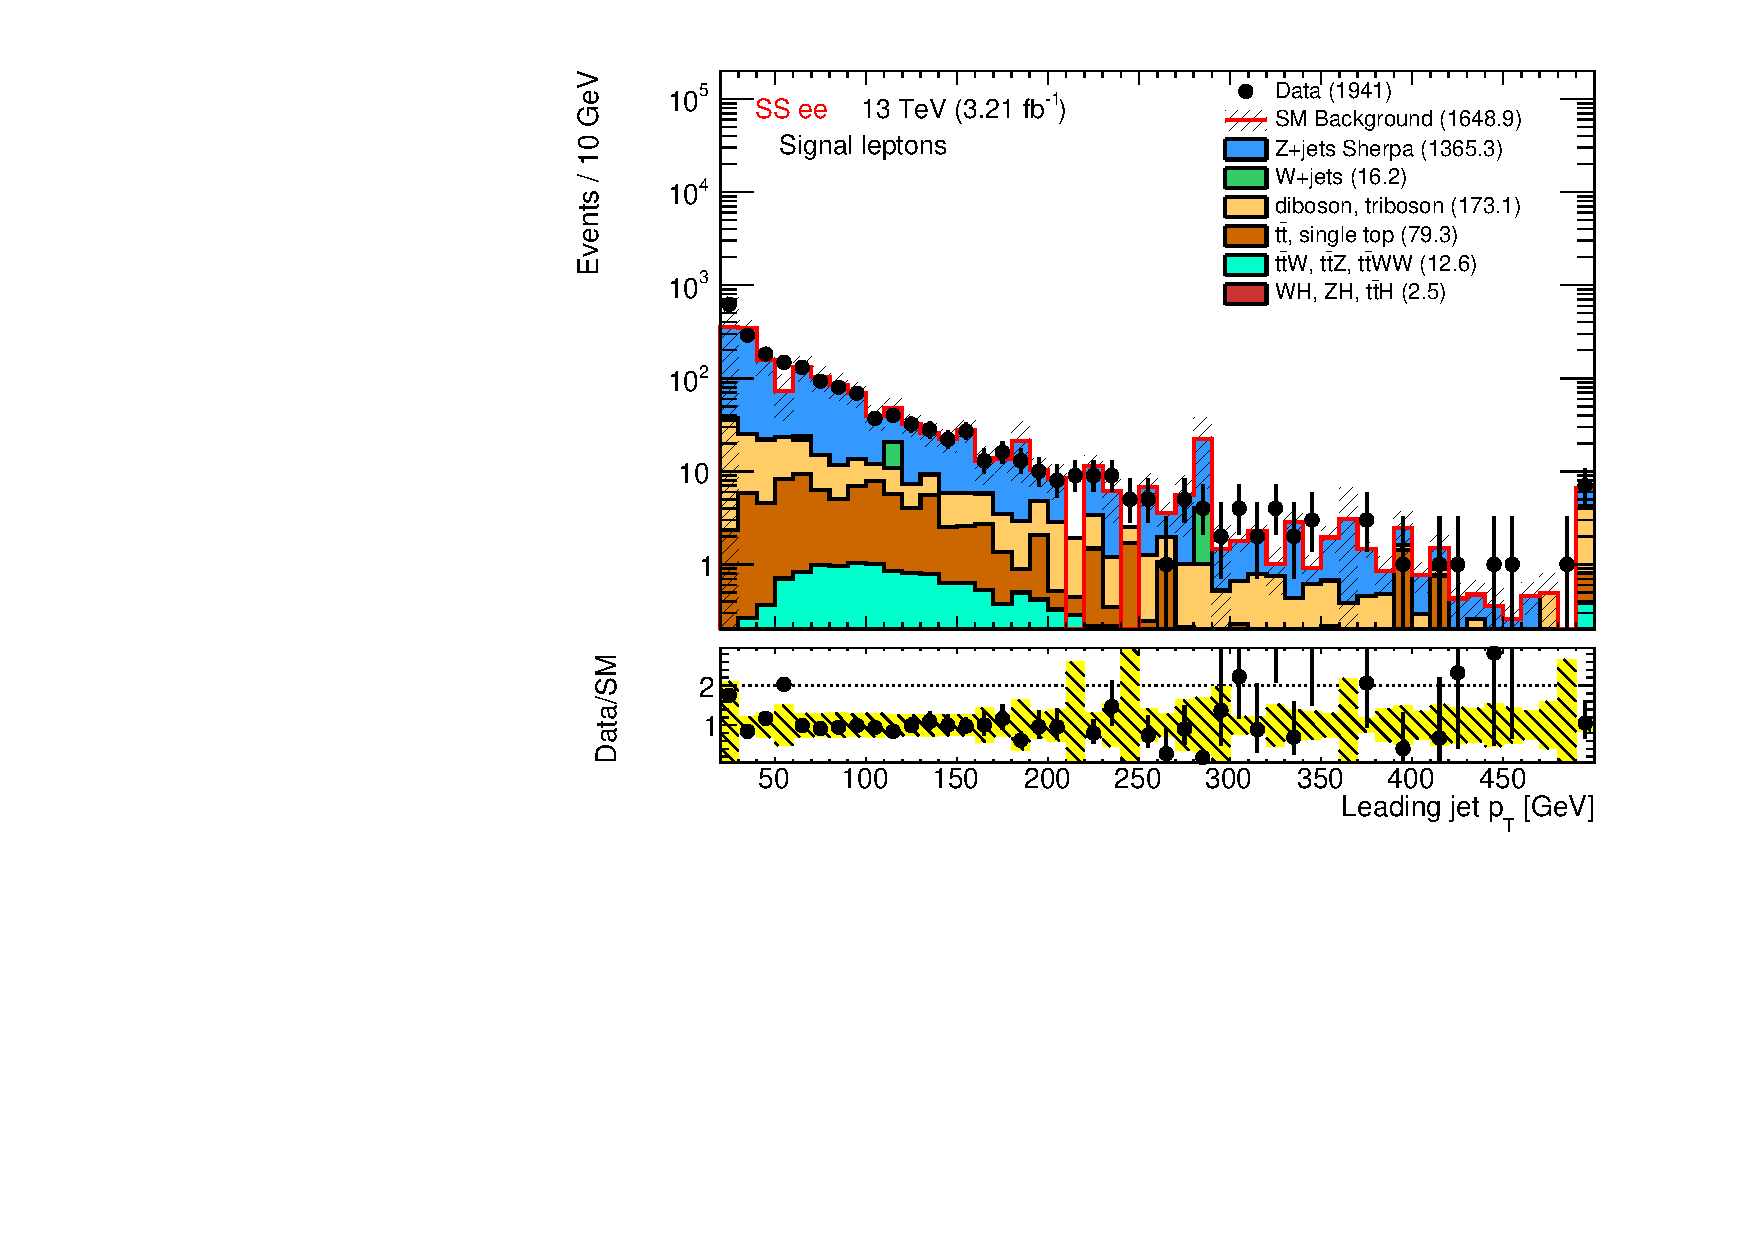
\includegraphics[width=0.49\textwidth]{DATAMC/PTJET1_afterlepton_SSee_0_physics.pdf}}
{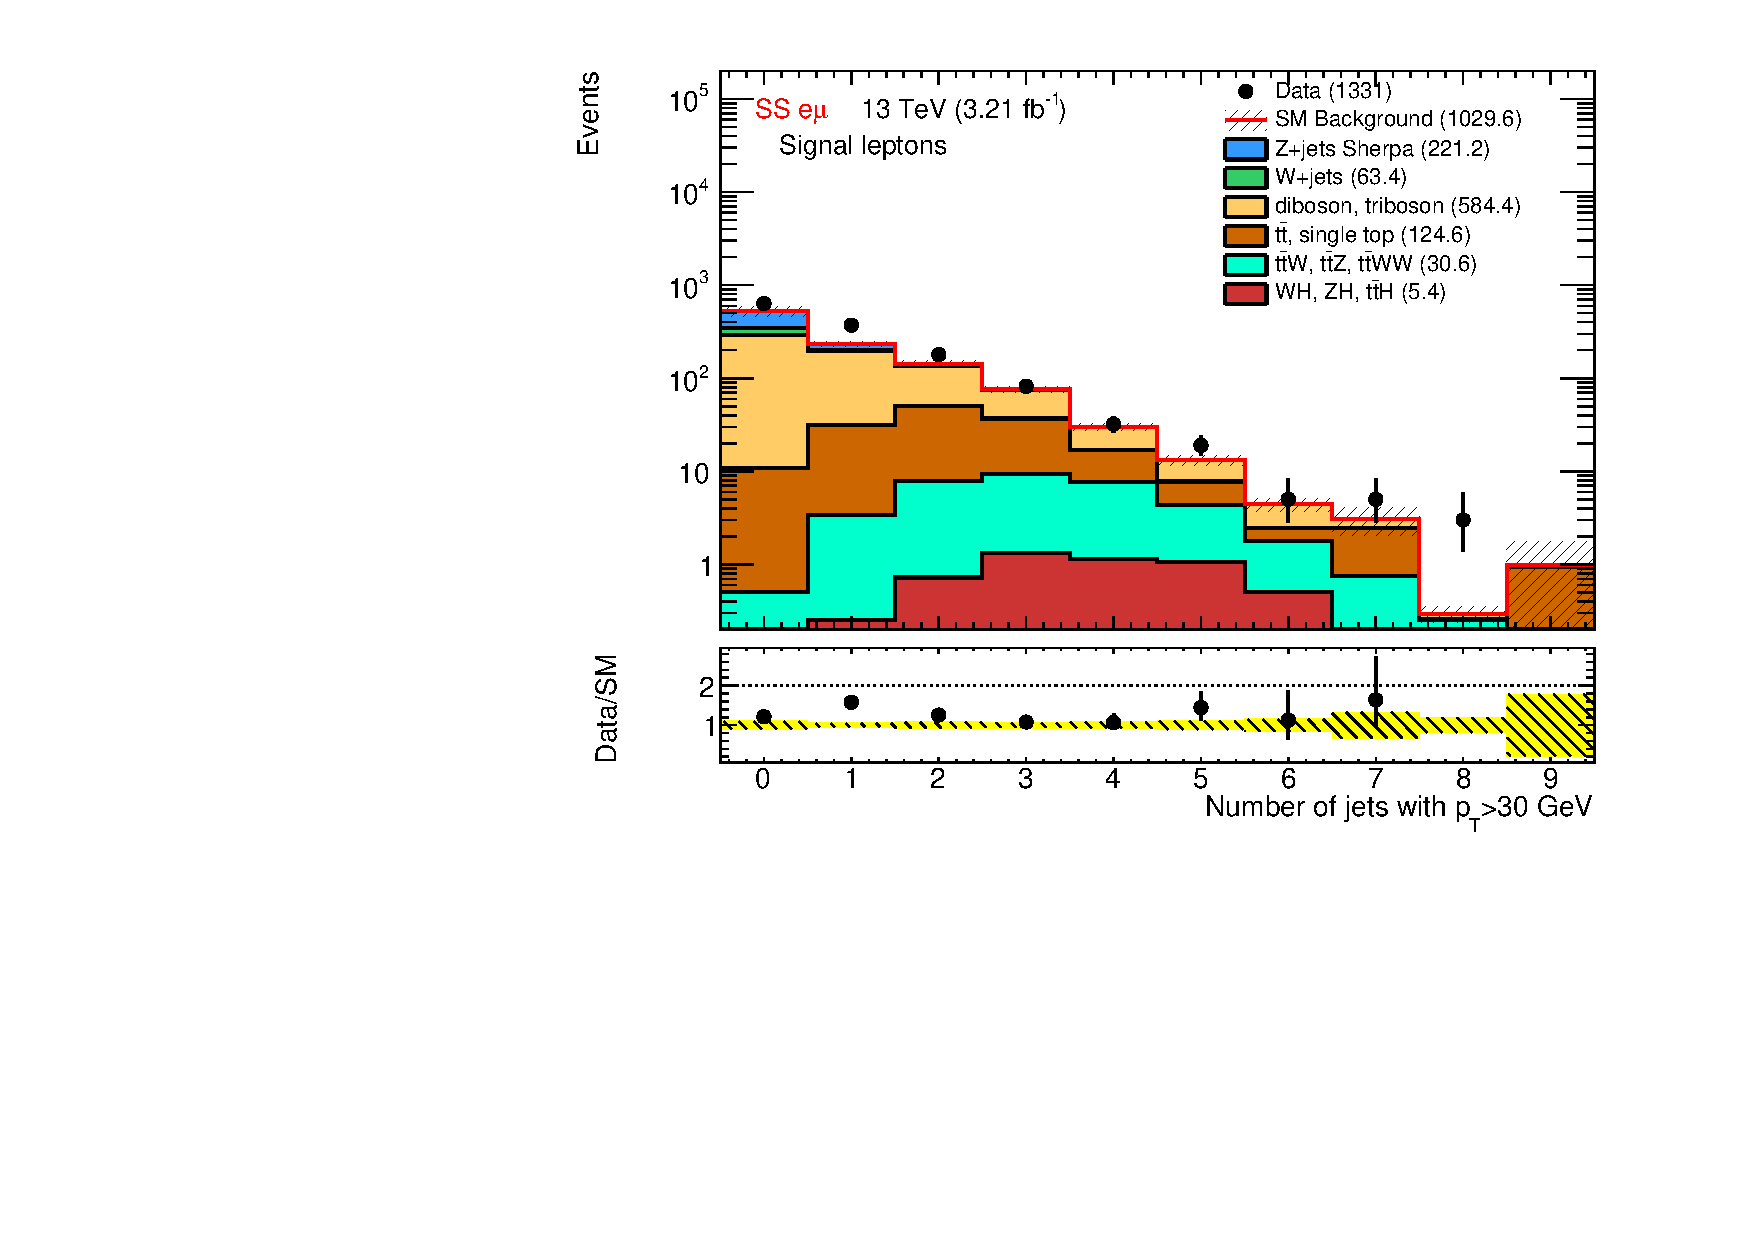
\includegraphics[width=0.49\textwidth]{DATAMC/NJET30_afterlepton_SSem_0_physics.pdf}}
{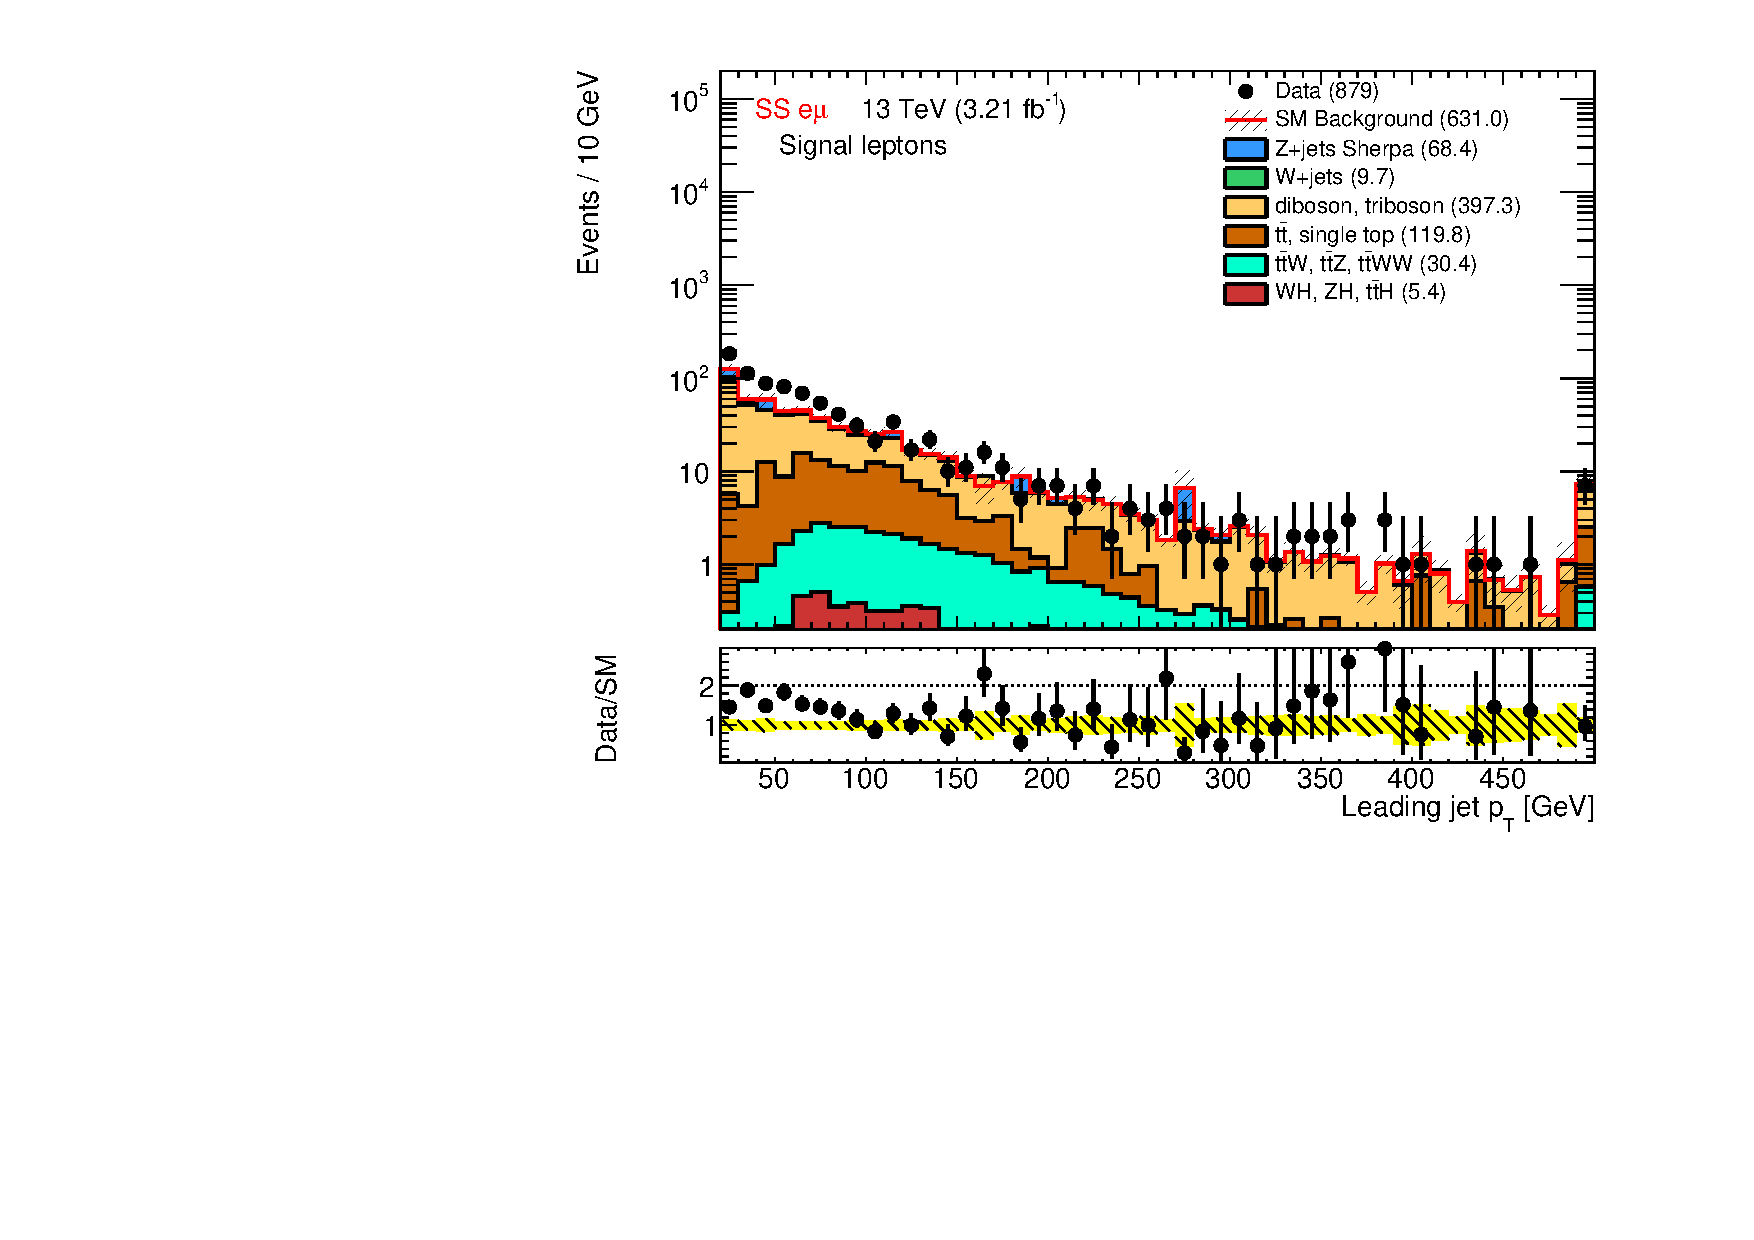
\includegraphics[width=0.49\textwidth]{DATAMC/PTJET1_afterlepton_SSem_0_physics.pdf}}
{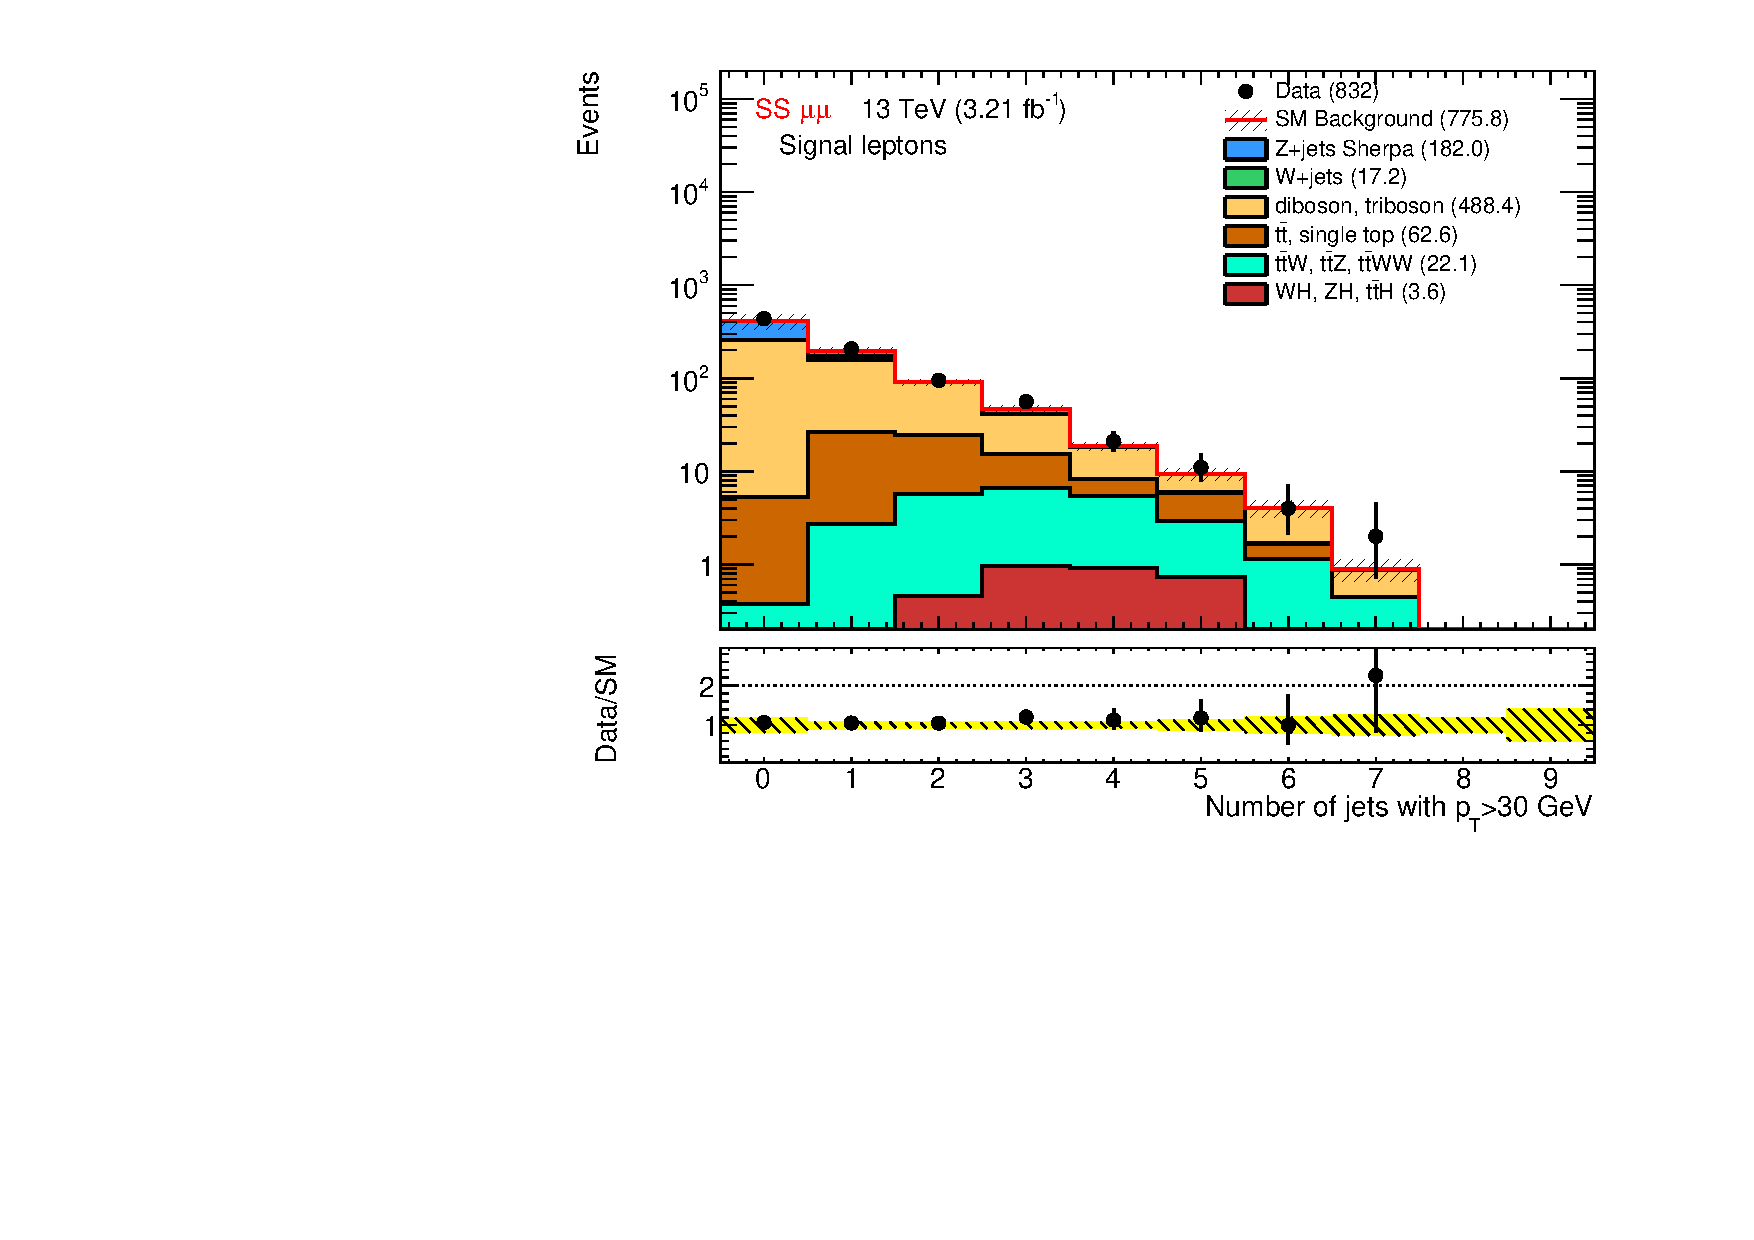
\includegraphics[width=0.49\textwidth]{DATAMC/NJET30_afterlepton_SSmm_0_physics.pdf}}
{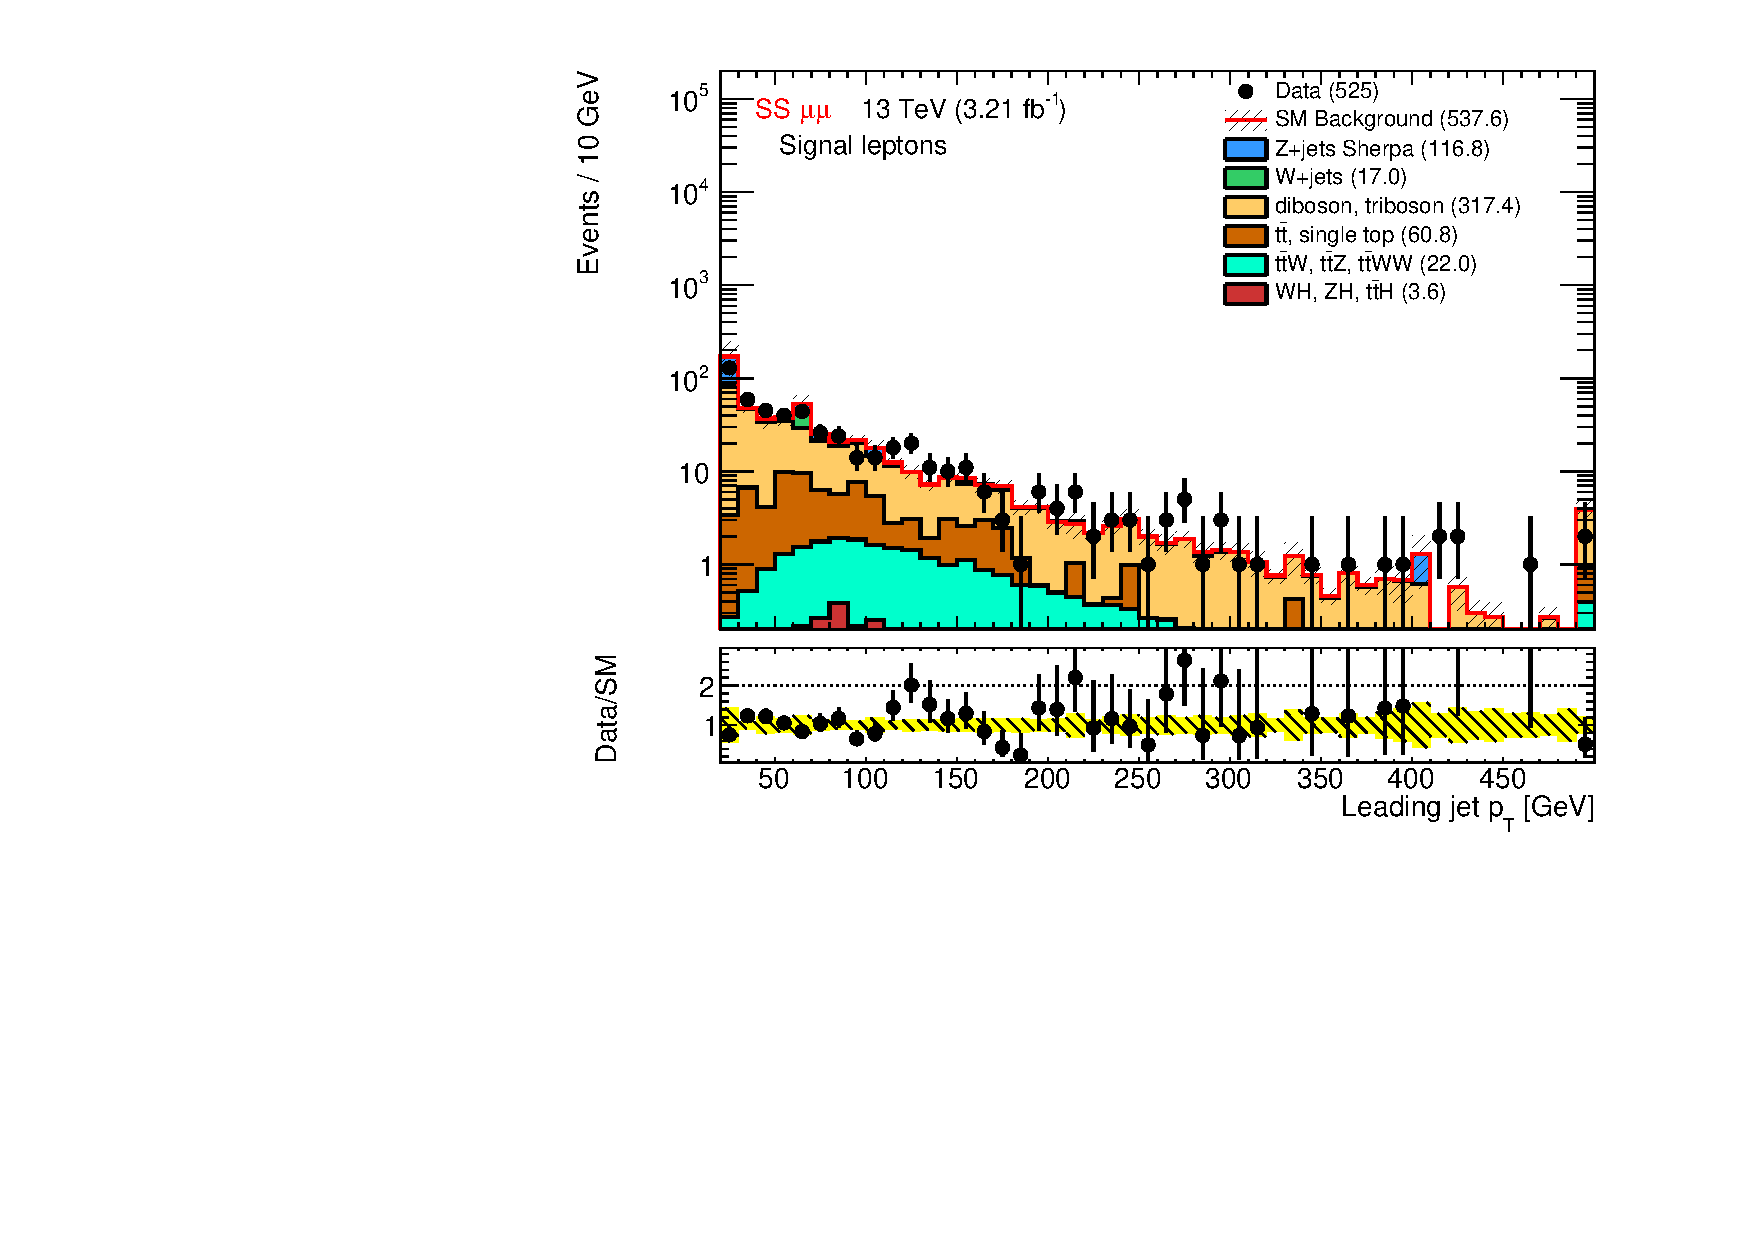
\includegraphics[width=0.49\textwidth]{DATAMC/PTJET1_afterlepton_SSmm_0_physics.pdf}}
\caption{Number of jets (left) and leading jet $\pt$ (right) for events selected in the $ee$ (top), $e\mu$ (center) and $\mu\mu$ (bottom) channels. The background contribution is taken directly from MC with no data-driven estimation of the background with fake and non-prompt leptons or charge mis-identification. Only luminosity and MC statistical uncertainties are included.
}
\label{fig:dataMC_jet}
\end{figure}


\begin{figure}[htb!]
\centering
{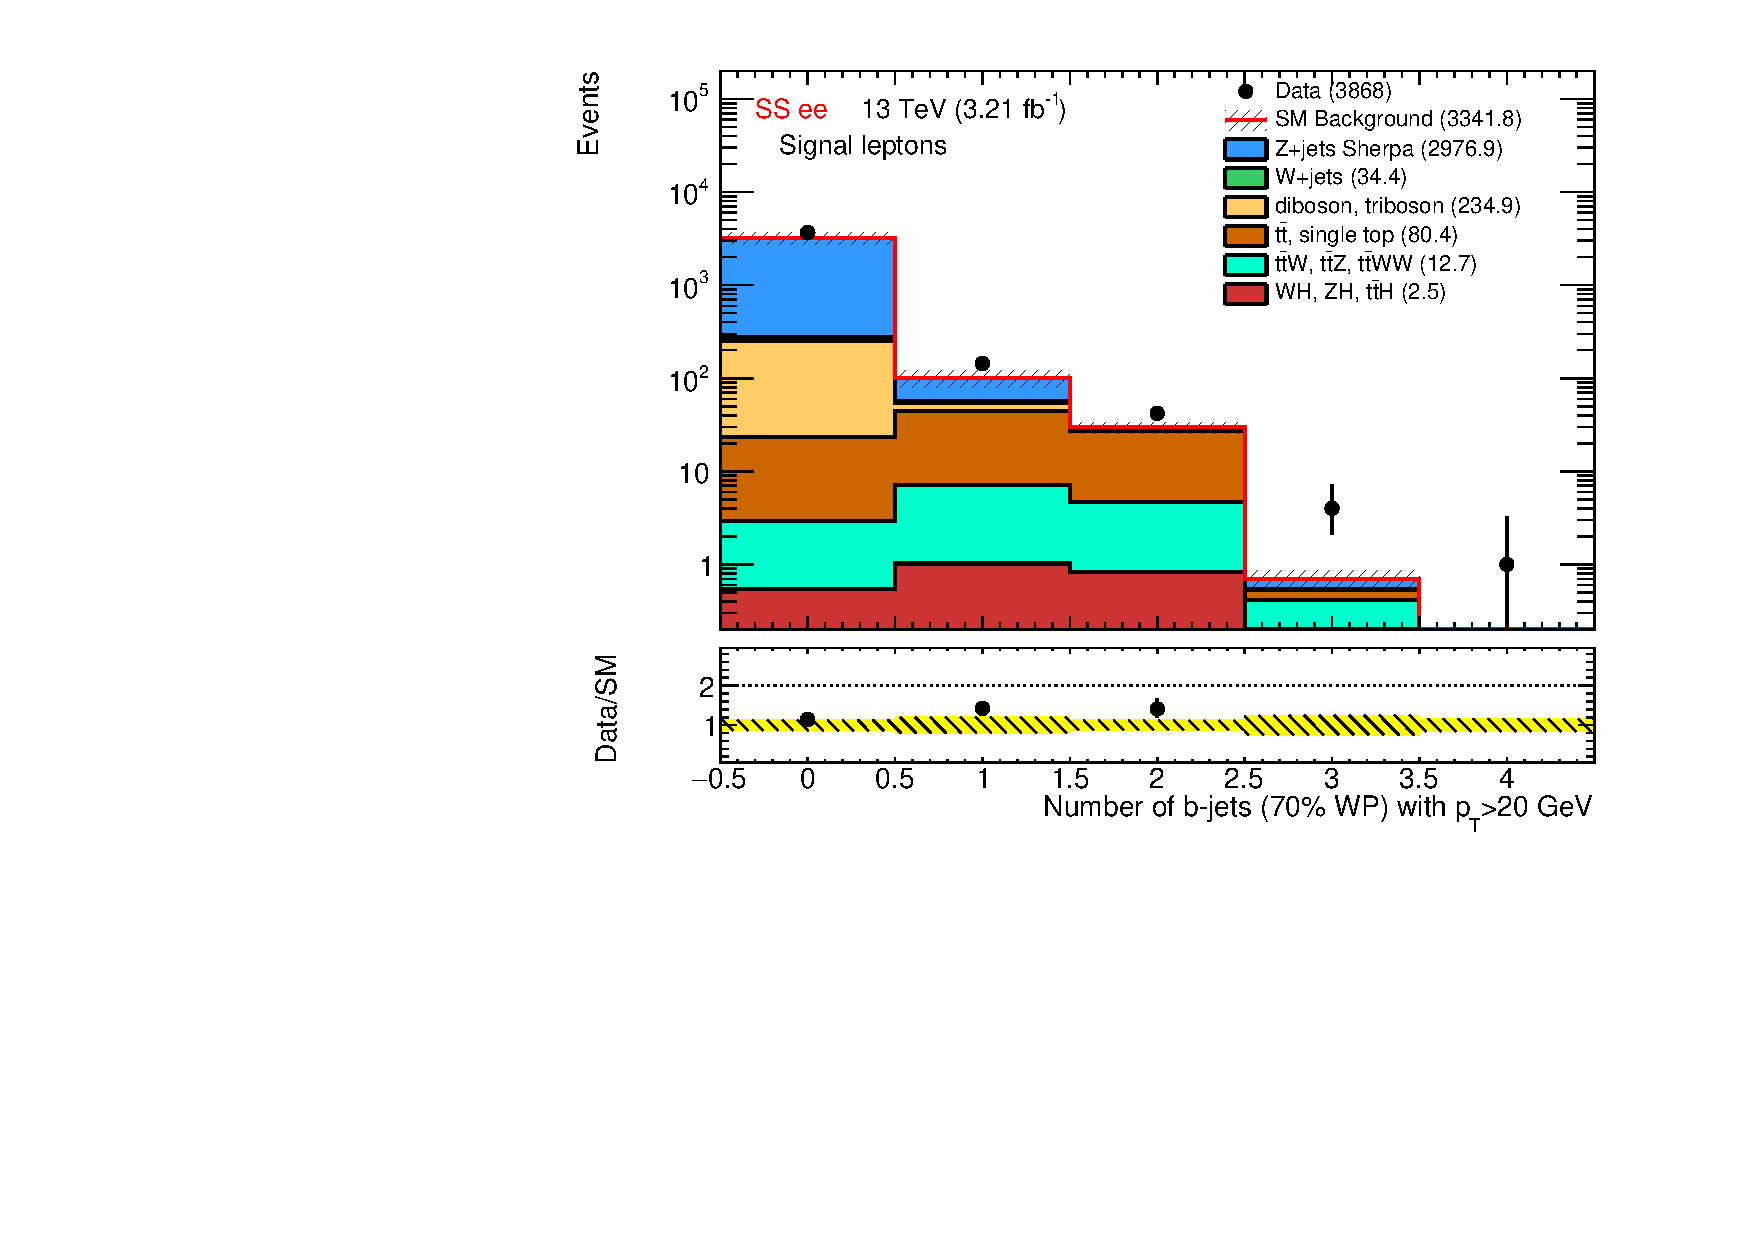
\includegraphics[width=0.49\textwidth]{DATAMC/NBJET70_20_afterlepton_SSee_0_physics.pdf}}
{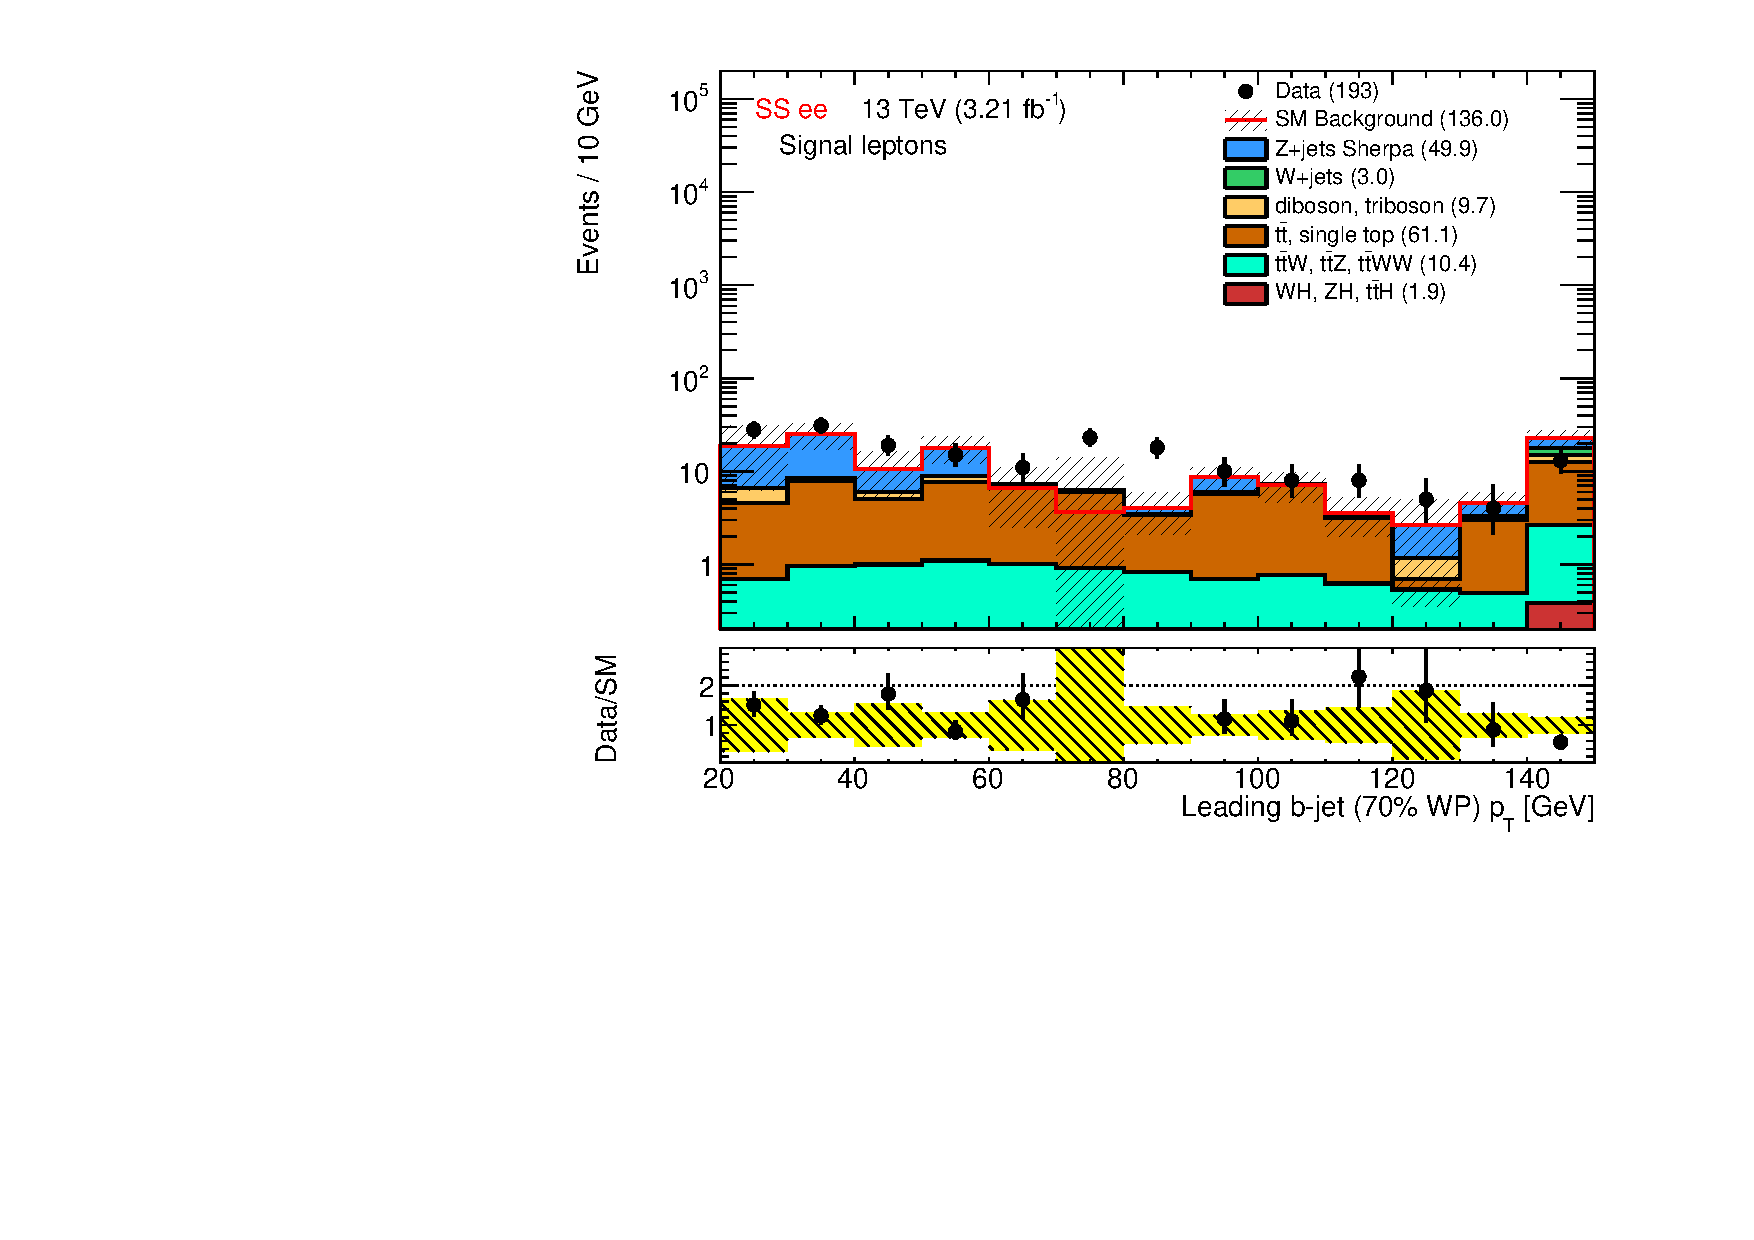
\includegraphics[width=0.49\textwidth]{DATAMC/PTBJET70_1_afterlepton_SSee_0_physics.pdf}}
{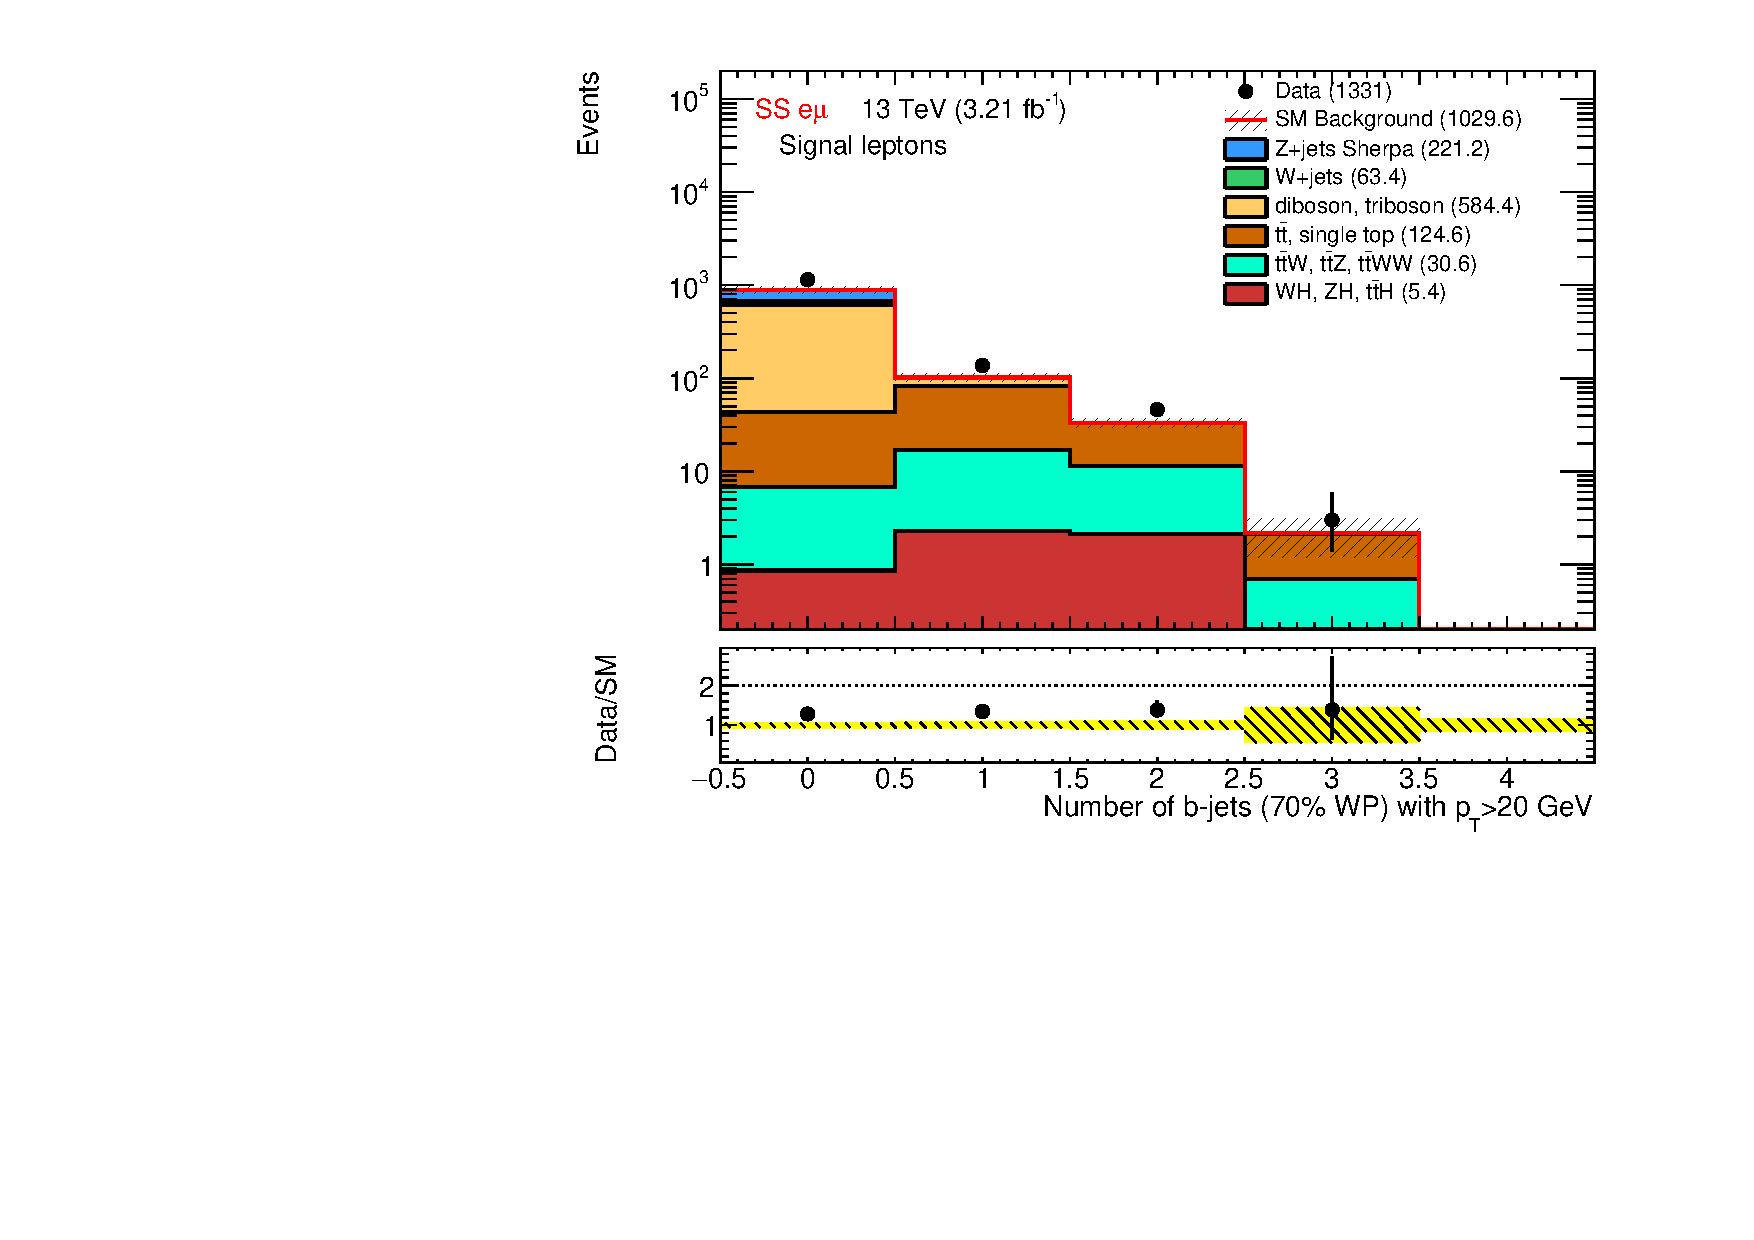
\includegraphics[width=0.49\textwidth]{DATAMC/NBJET70_20_afterlepton_SSem_0_physics.pdf}}
{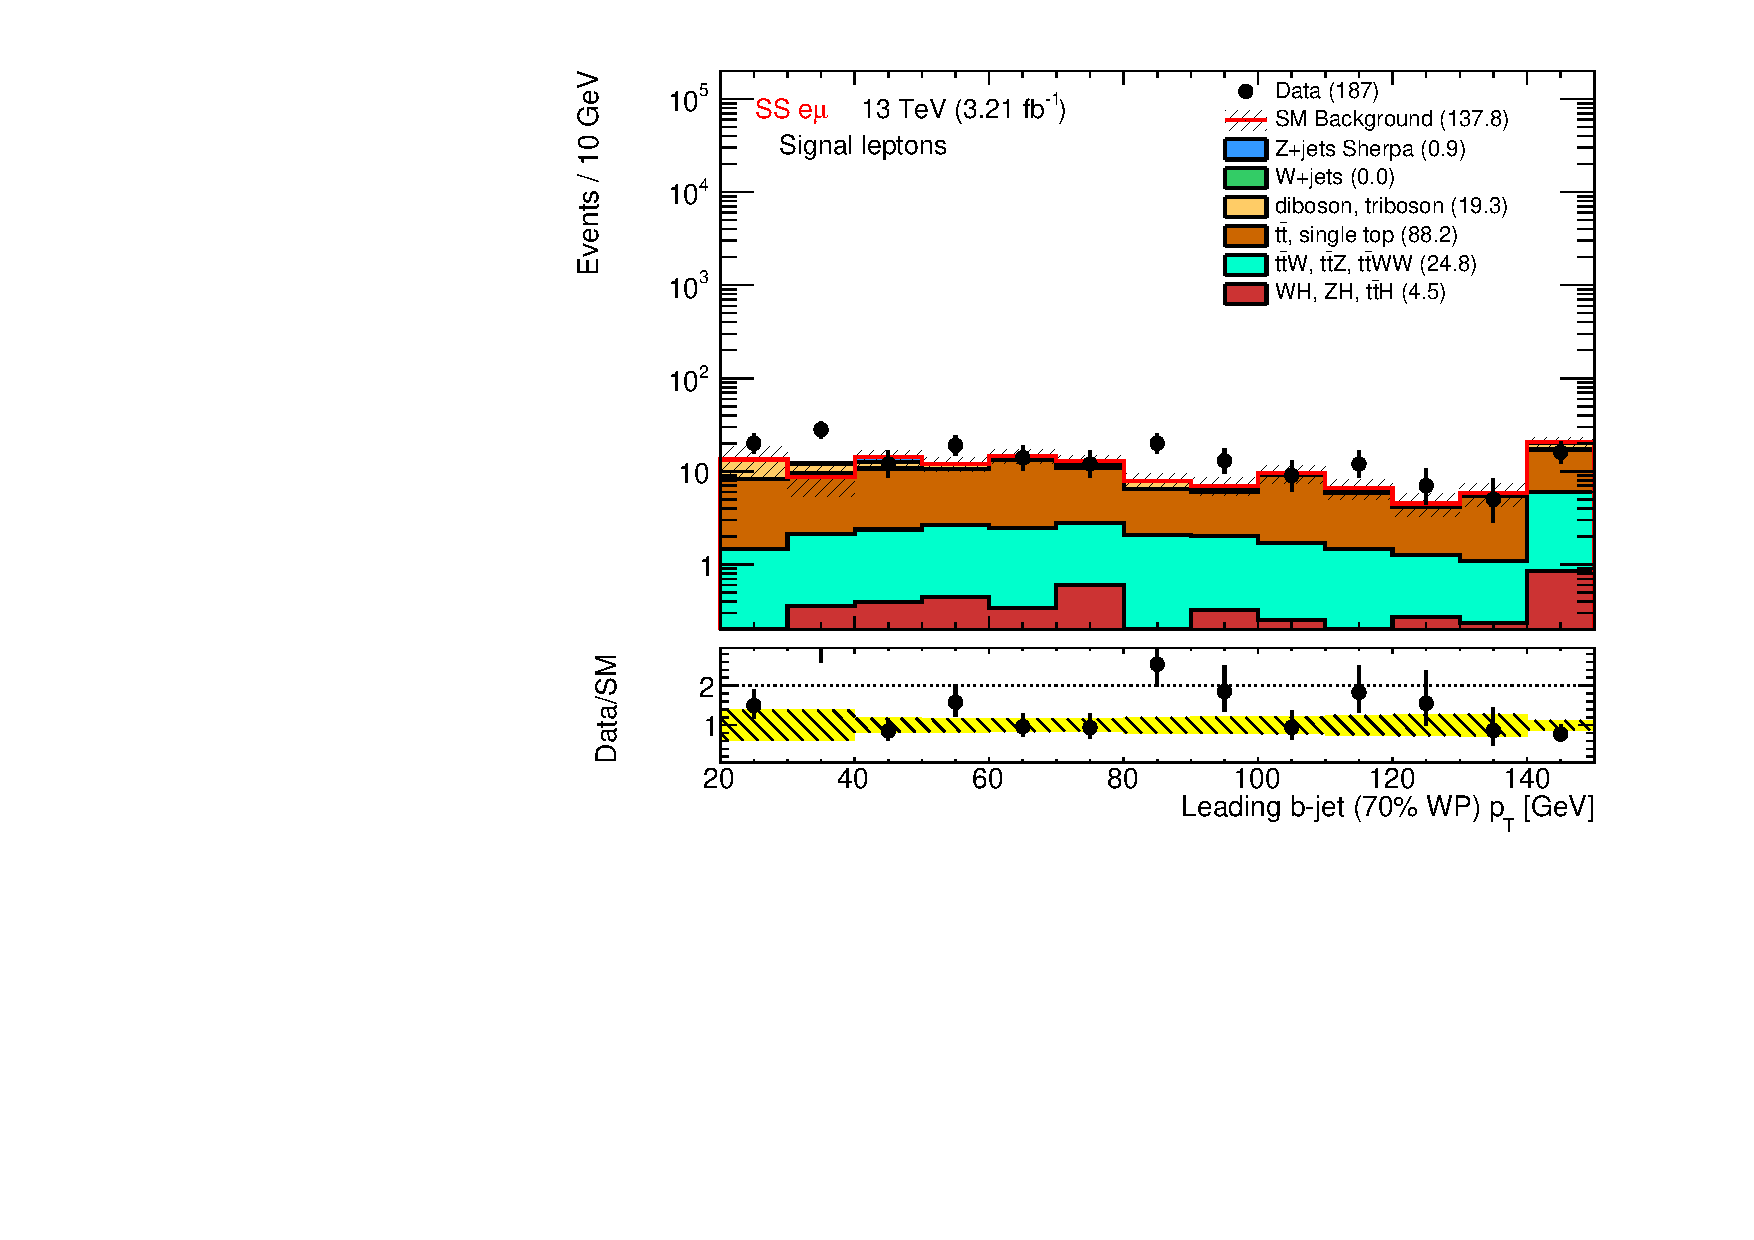
\includegraphics[width=0.49\textwidth]{DATAMC/PTBJET70_1_afterlepton_SSem_0_physics.pdf}}
{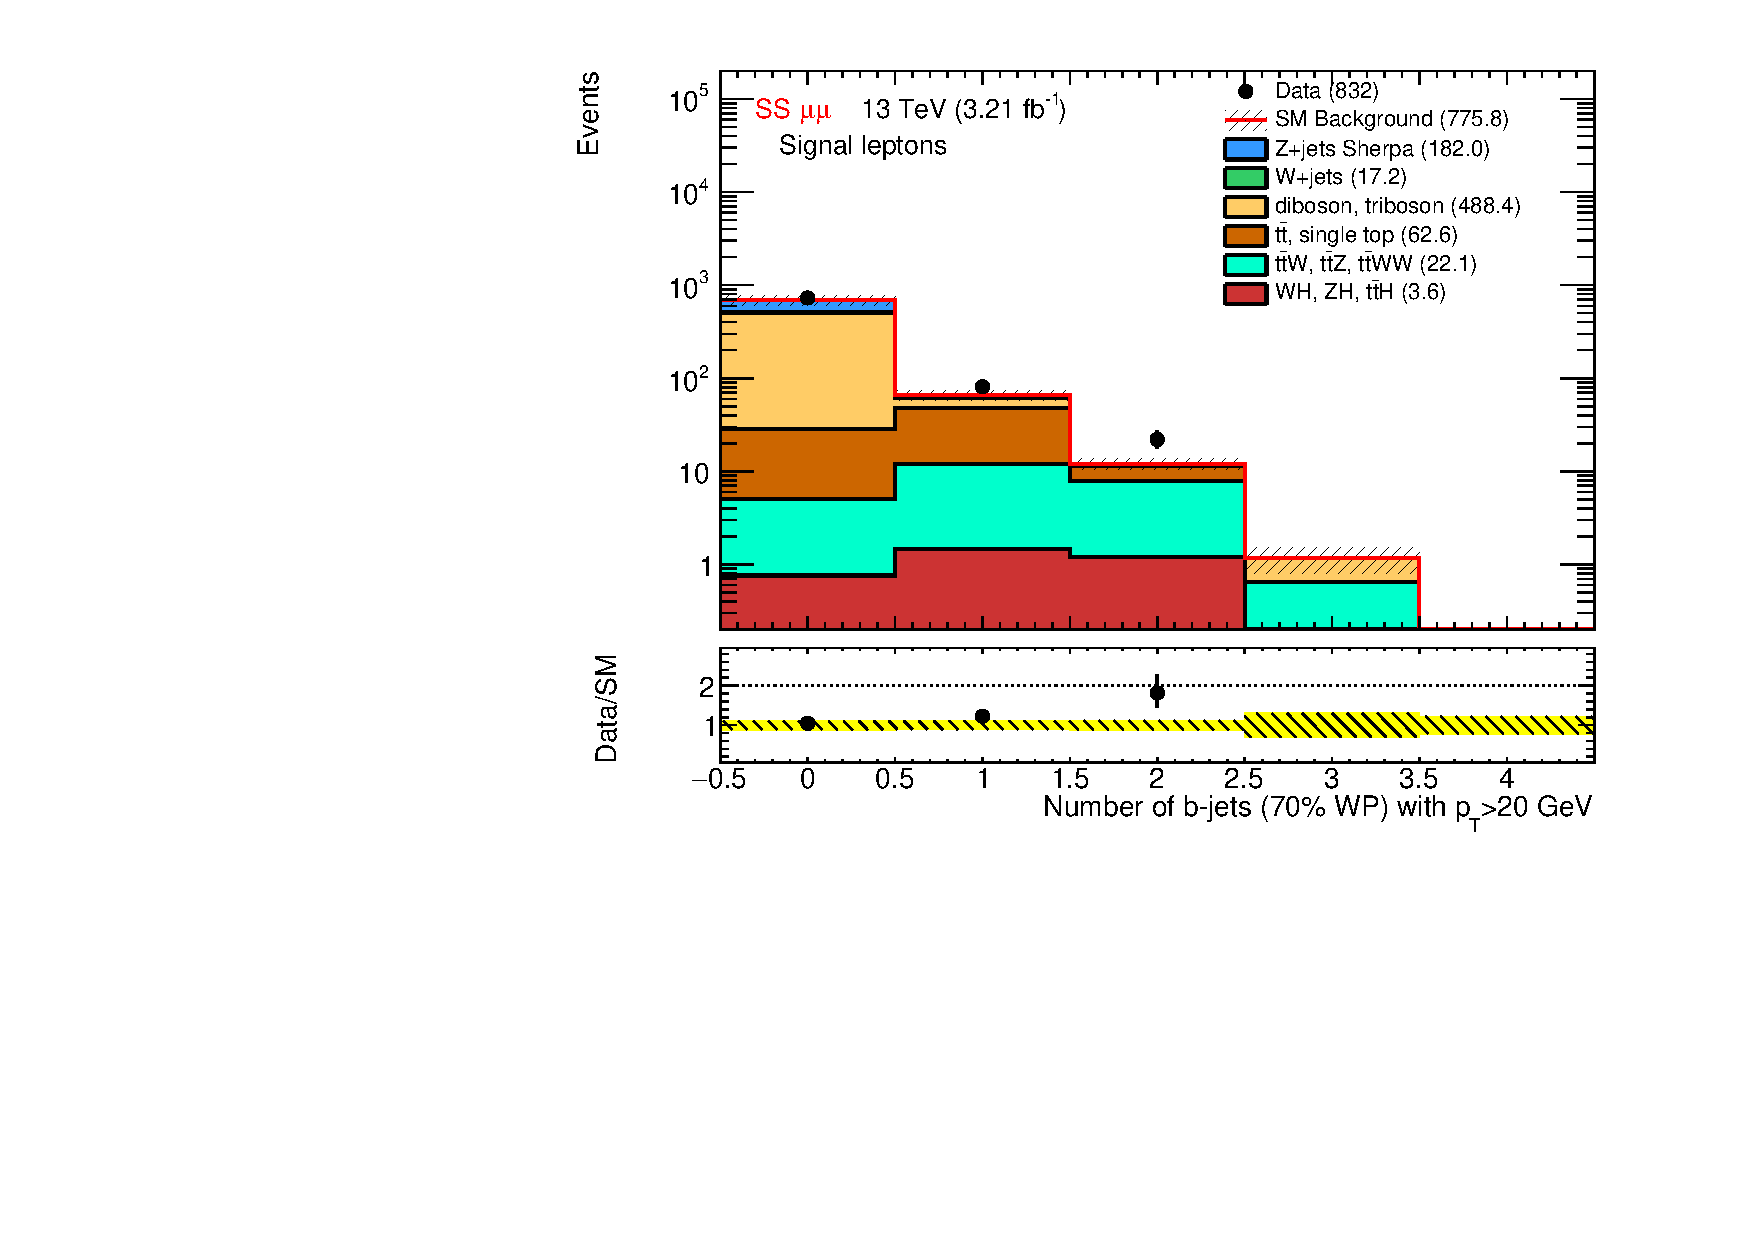
\includegraphics[width=0.49\textwidth]{DATAMC/NBJET70_20_afterlepton_SSmm_0_physics.pdf}}
{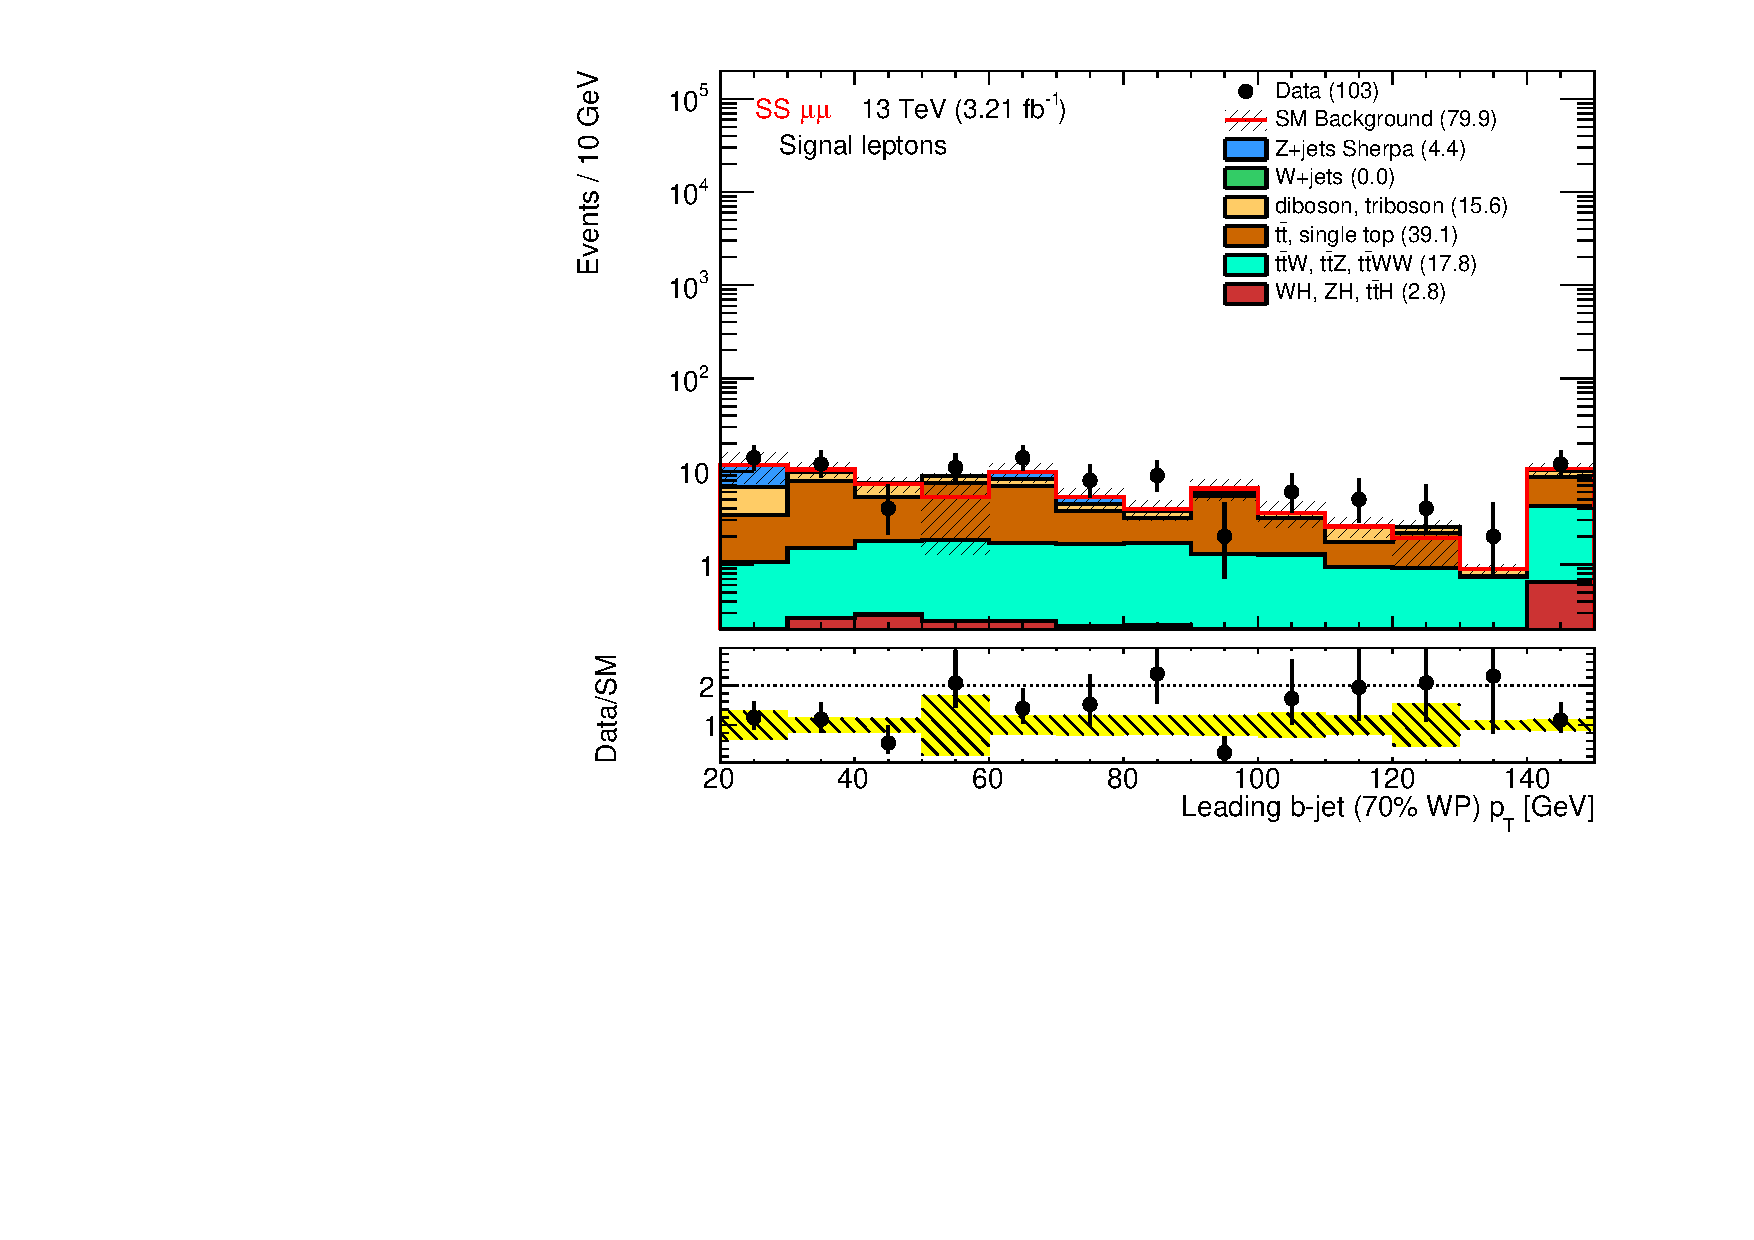
\includegraphics[width=0.49\textwidth]{DATAMC/PTBJET70_1_afterlepton_SSmm_0_physics.pdf}}
\caption{Number of $b$-jets (left) and leading $b$-jet $\pt$ (right) for events selected in the $ee$ (top), $e\mu$ (center) and $\mu\mu$ (bottom) channels. The background contribution is taken directly from MC with no data-driven estimation of the background with fake and non-prompt leptons or charge mis-identification. Only luminosity and MC statistical uncertainties are included.
}
\label{fig:dataMC_bjet}
\end{figure}


\begin{figure}[htb!]
\centering
{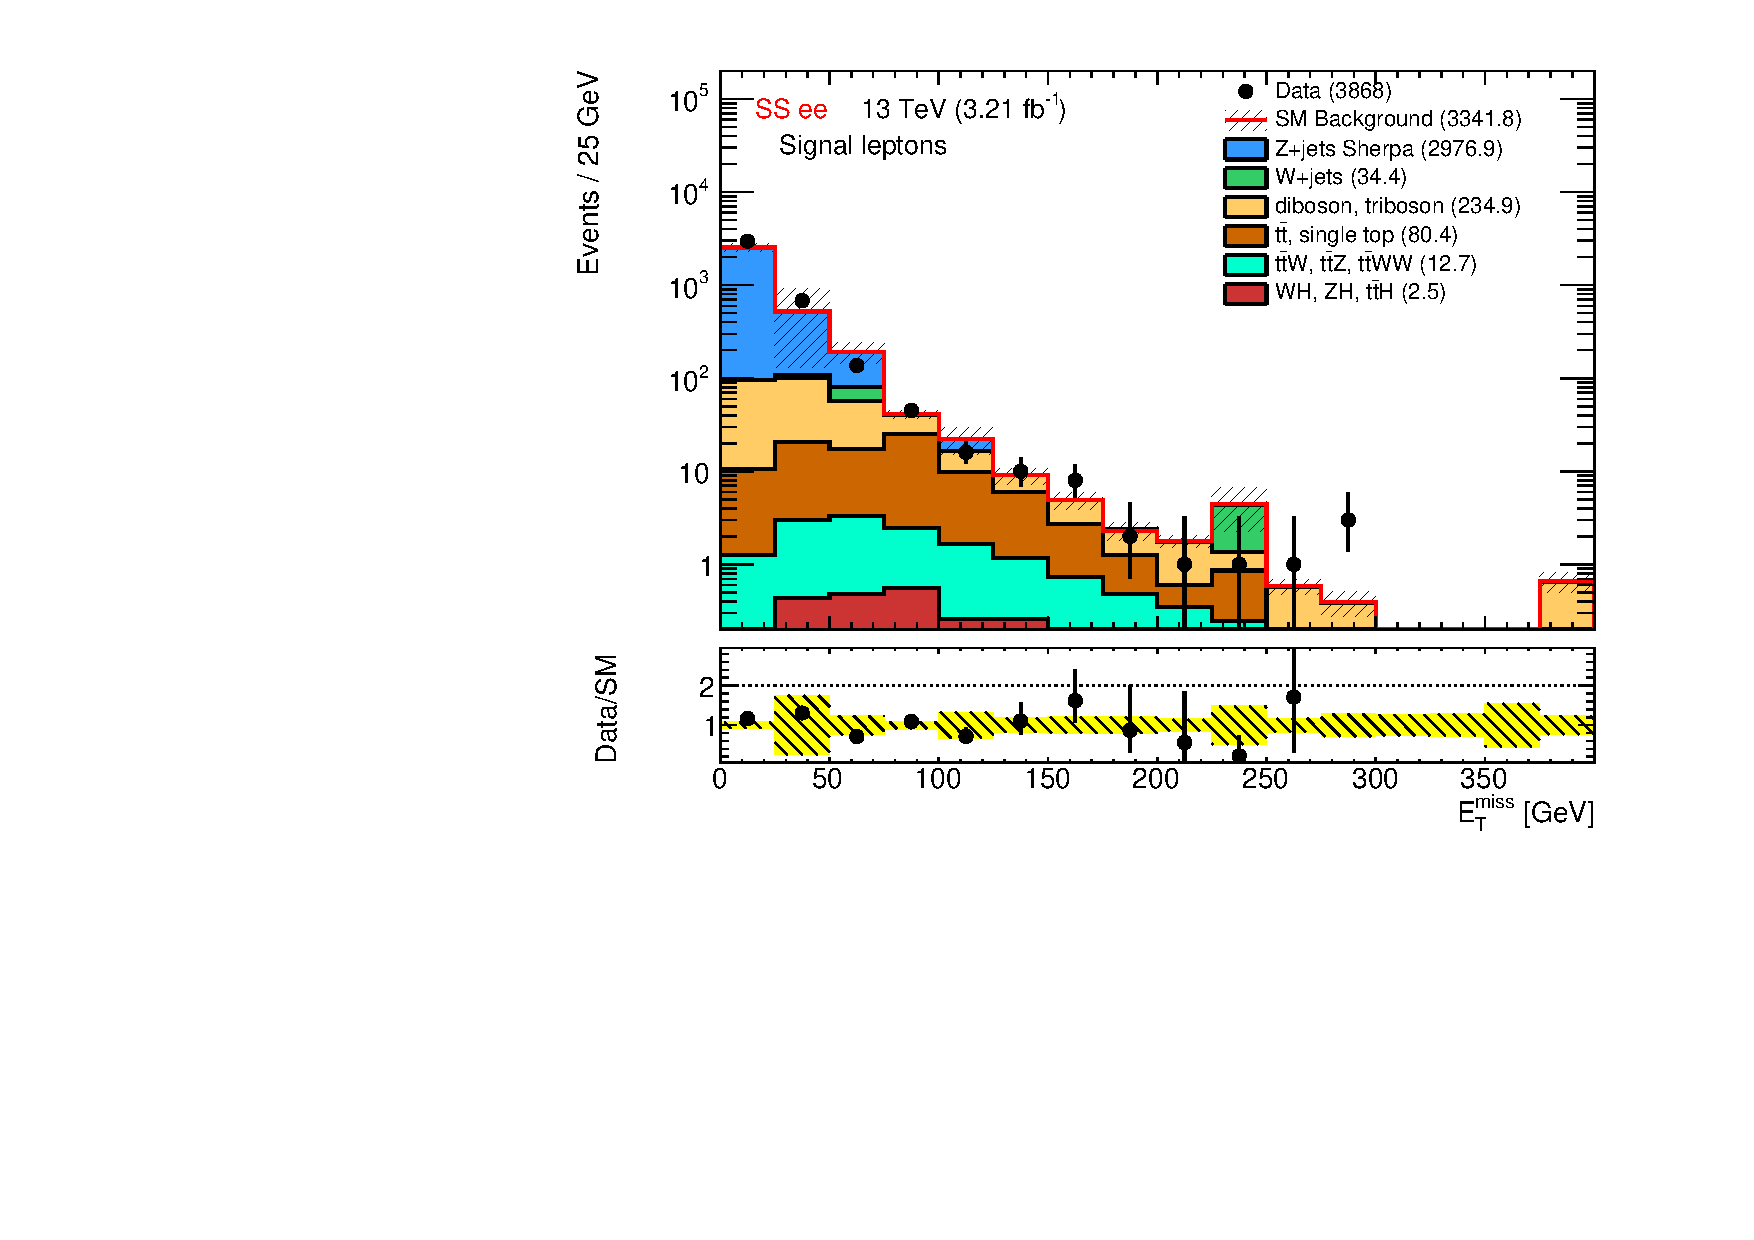
\includegraphics[width=0.49\textwidth]{DATAMC/MET_afterlepton_SSee_0_physics.pdf}}
{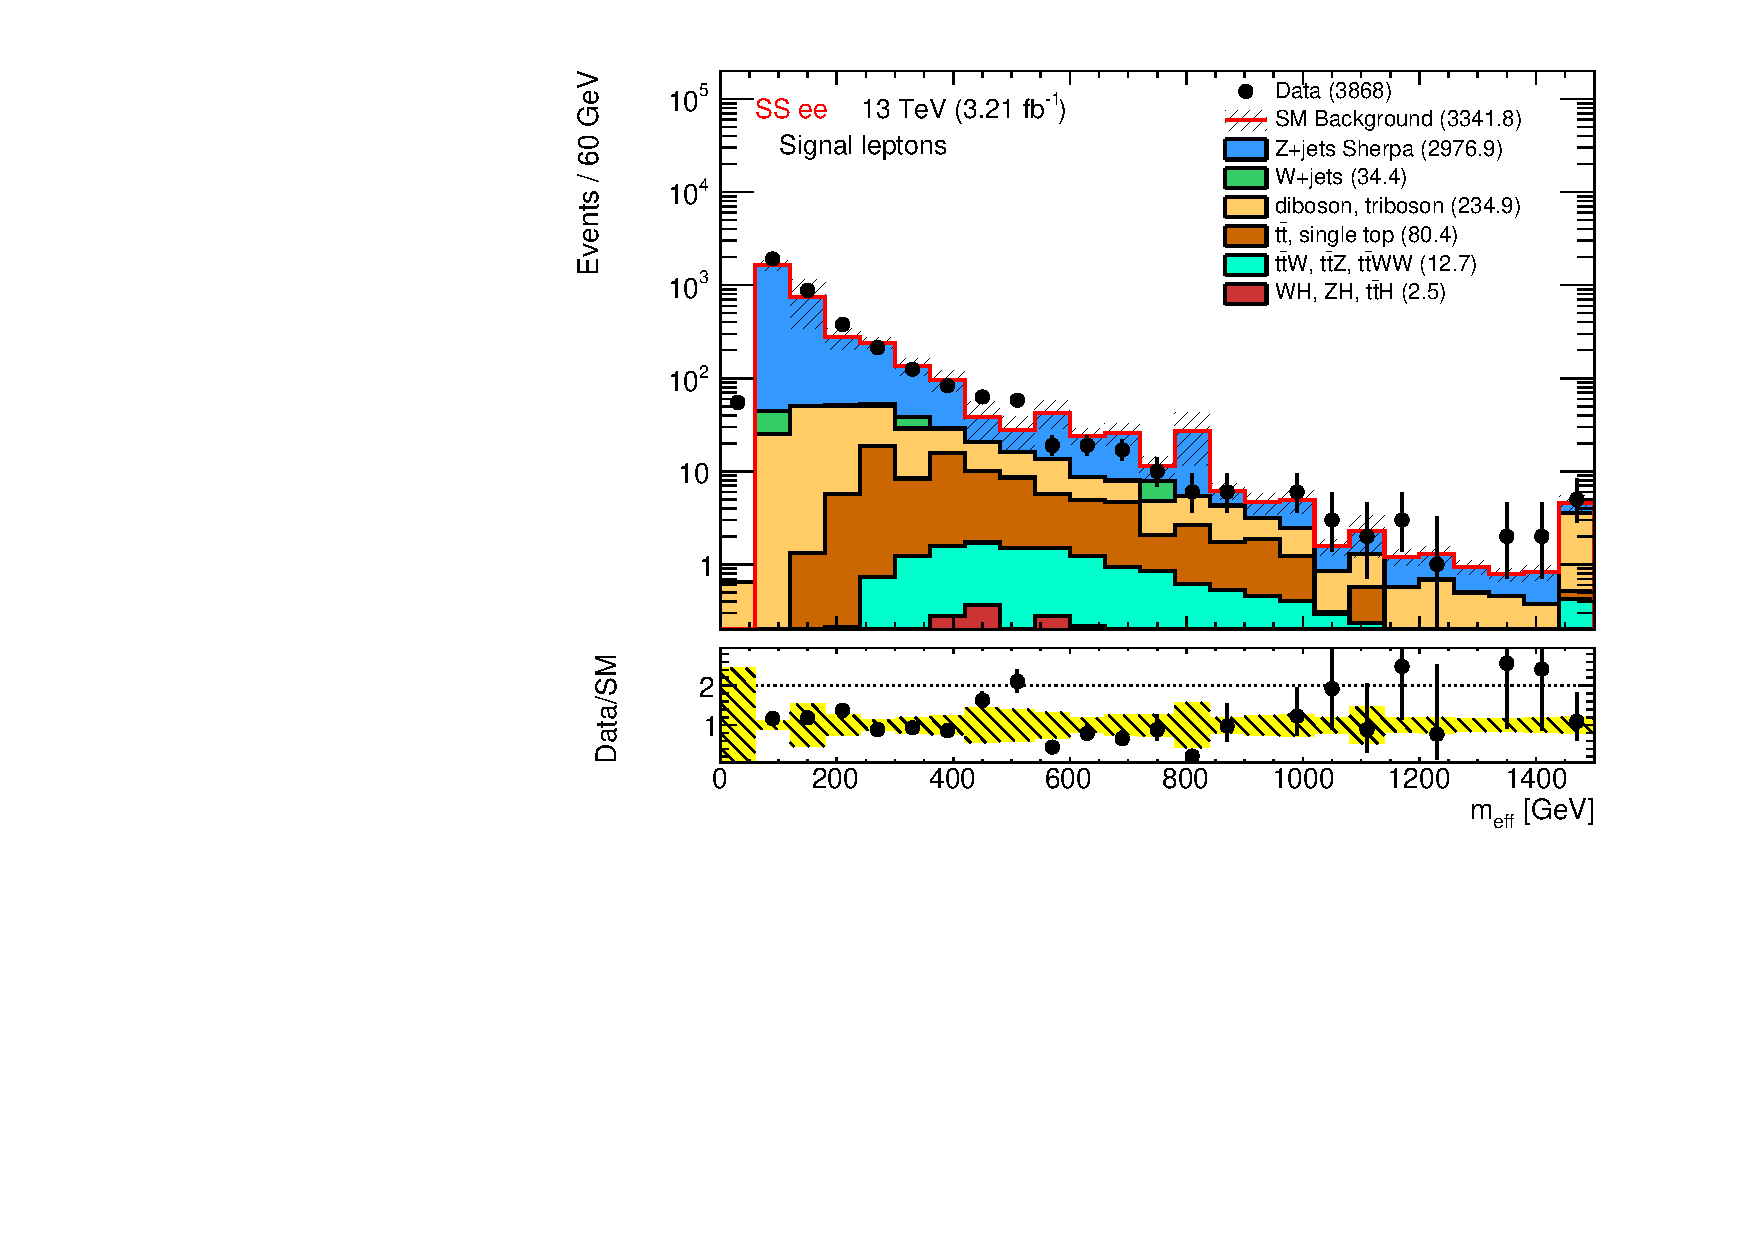
\includegraphics[width=0.49\textwidth]{DATAMC/MEFF_afterlepton_SSee_0_physics.pdf}}
{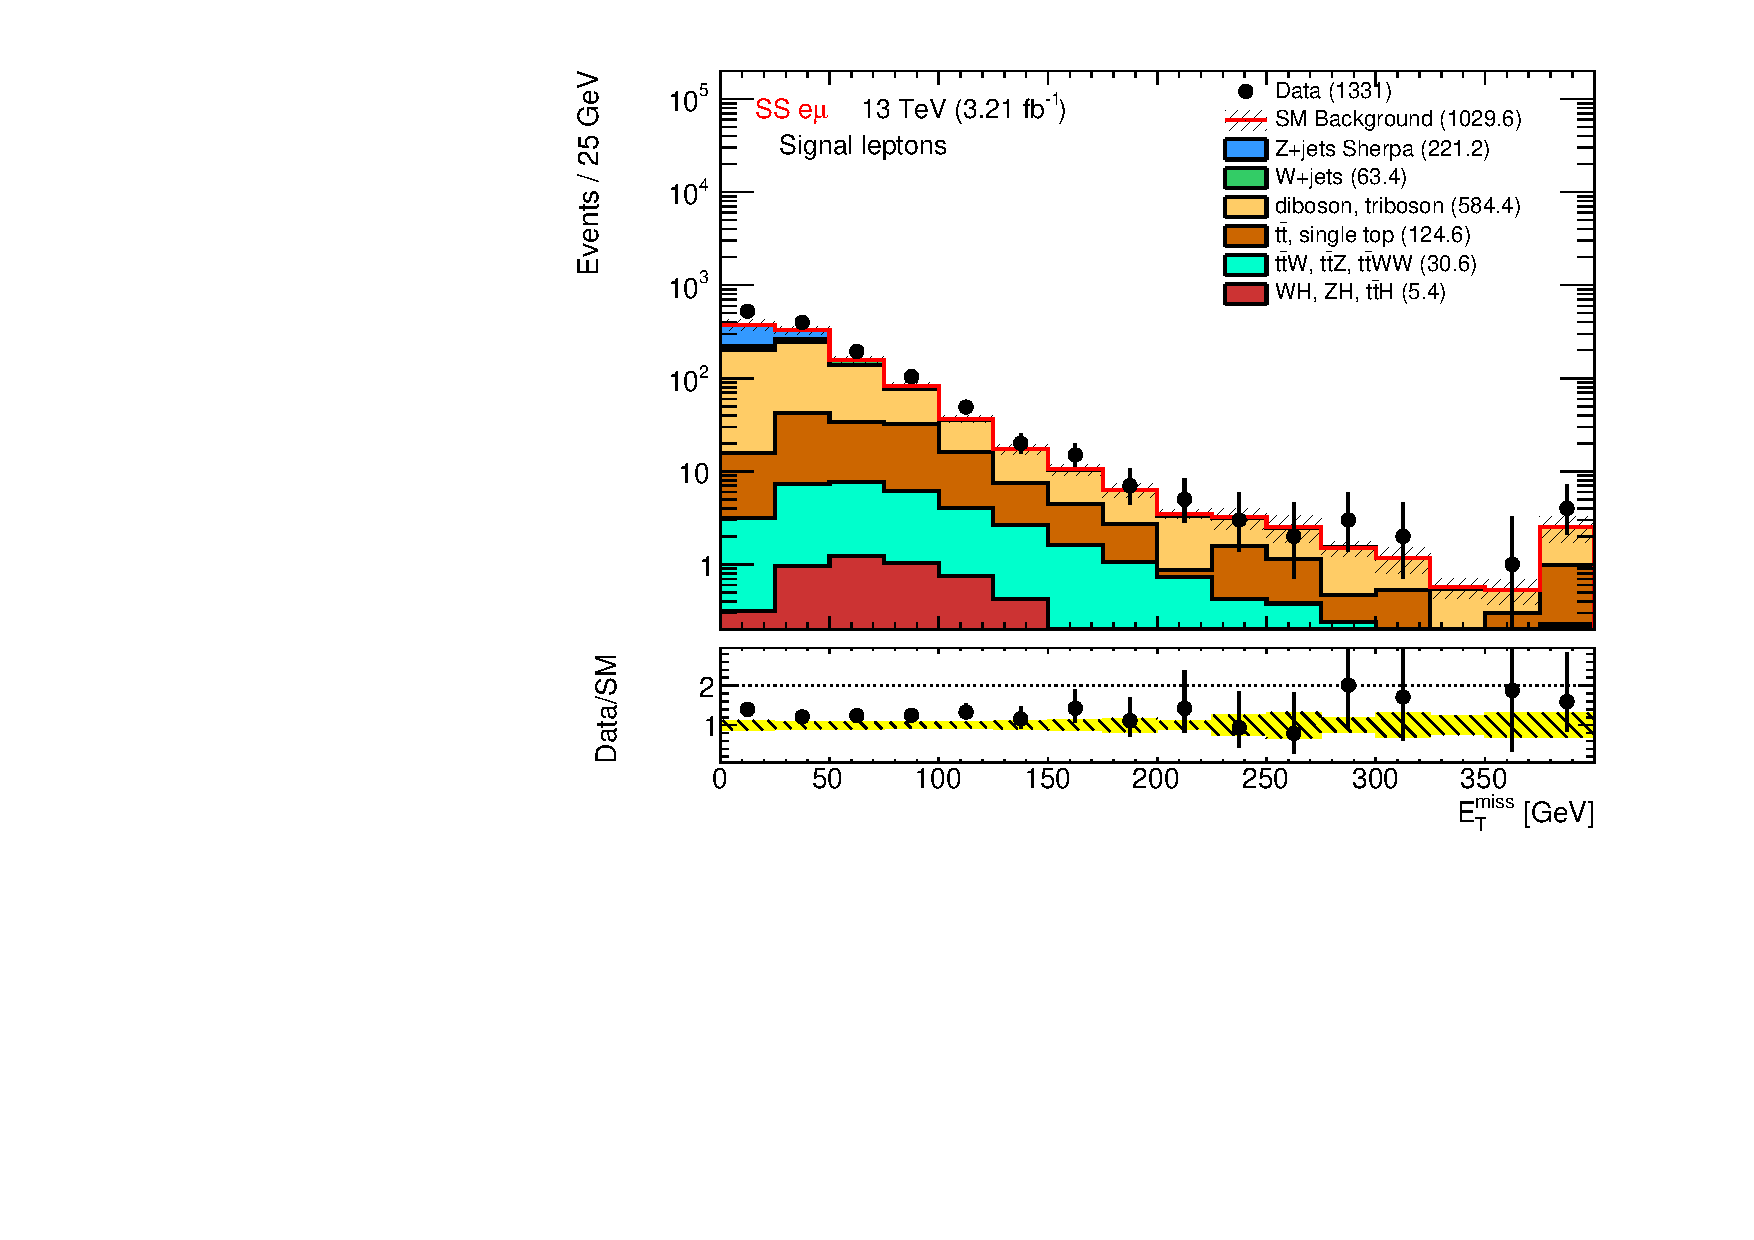
\includegraphics[width=0.49\textwidth]{DATAMC/MET_afterlepton_SSem_0_physics.pdf}}
{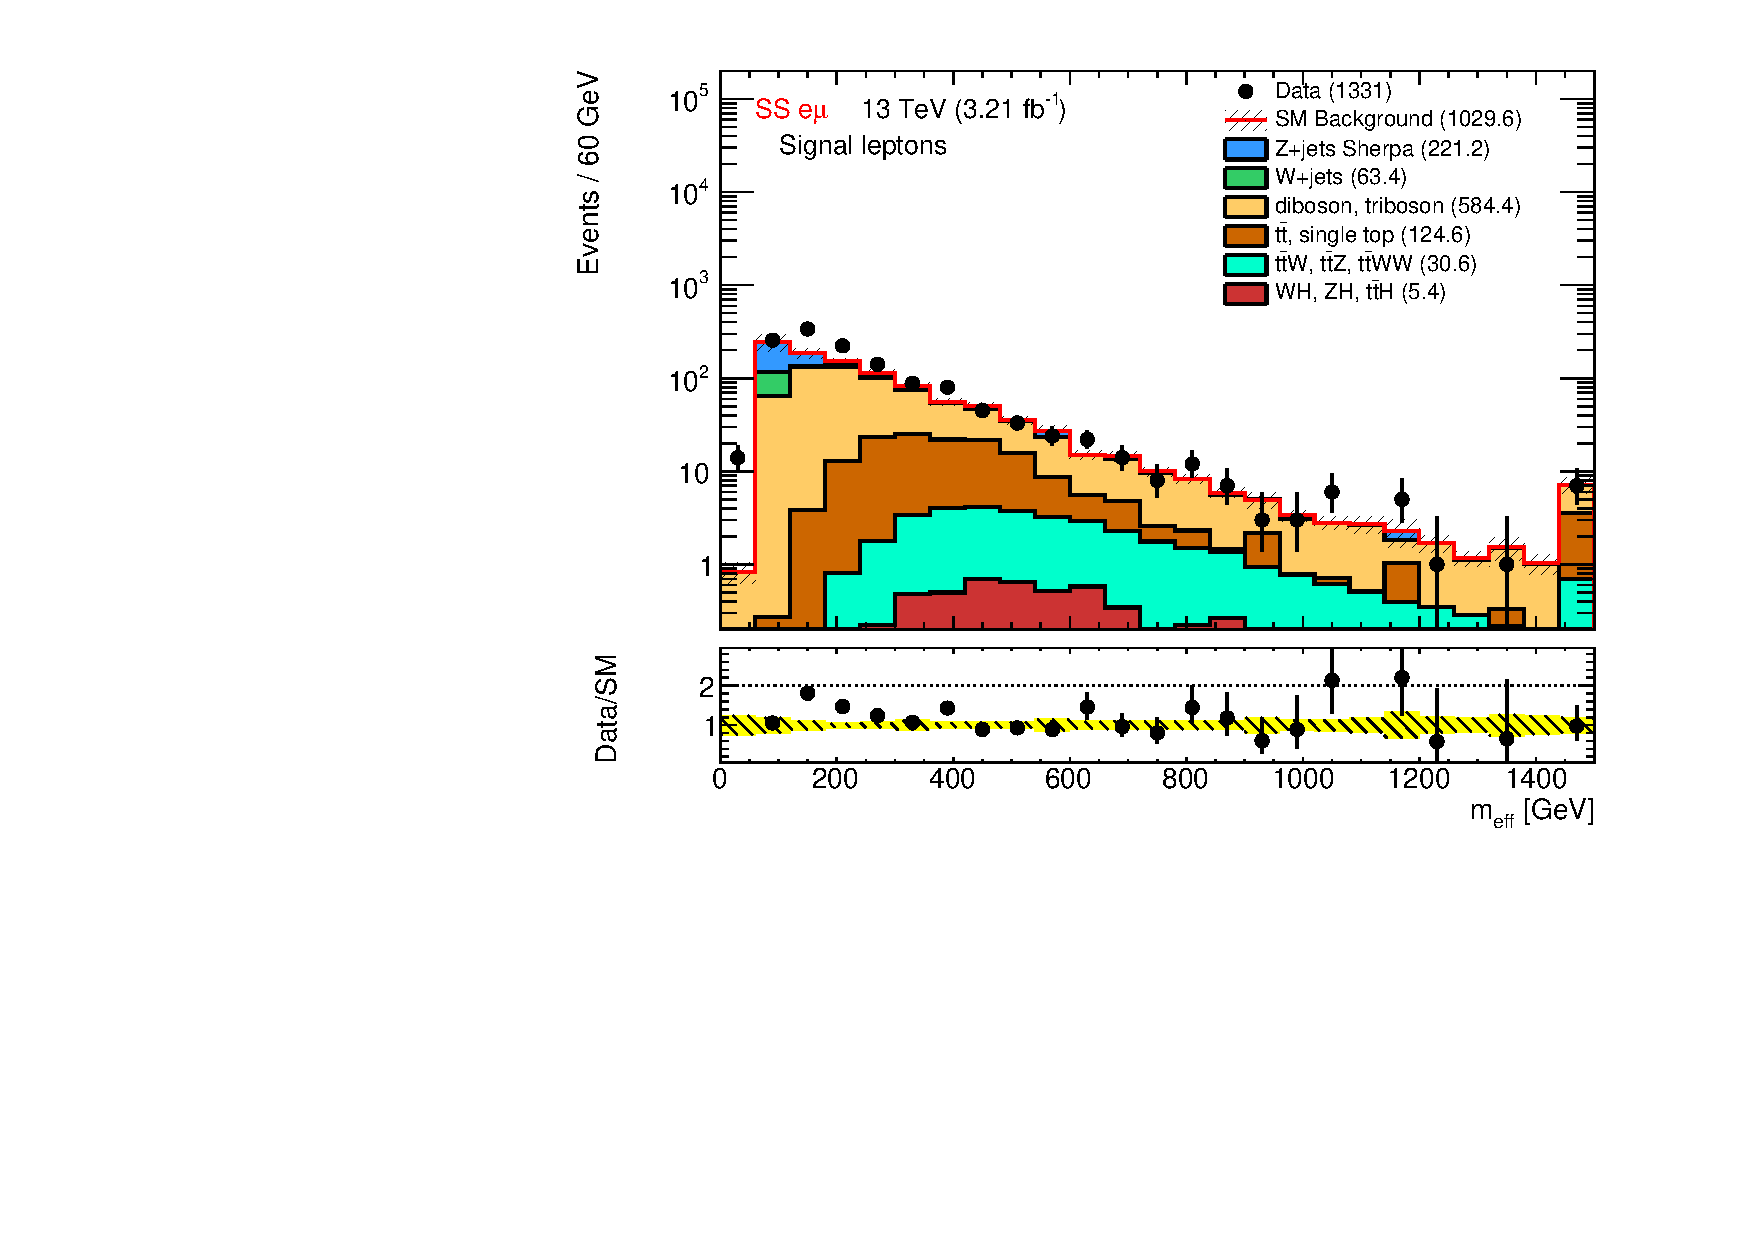
\includegraphics[width=0.49\textwidth]{DATAMC/MEFF_afterlepton_SSem_0_physics.pdf}}
{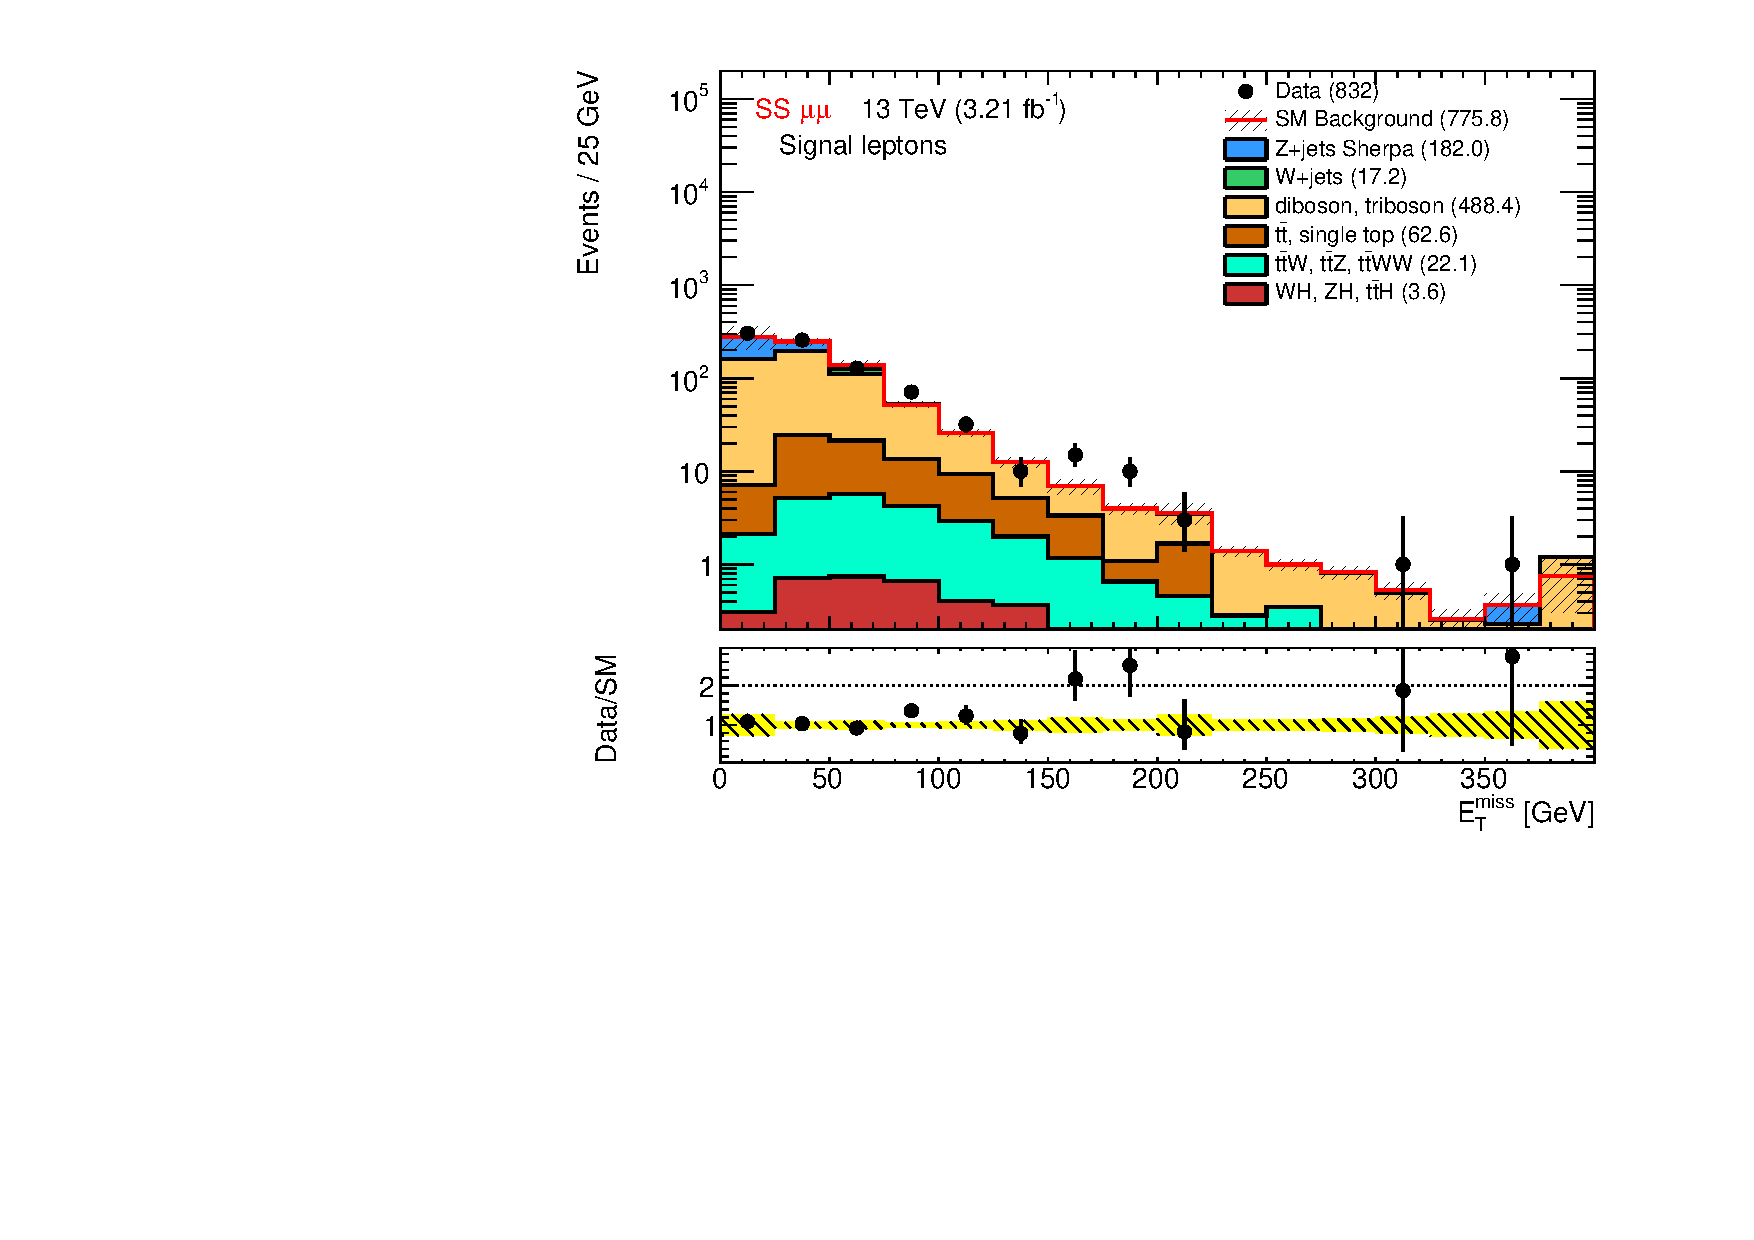
\includegraphics[width=0.49\textwidth]{DATAMC/MET_afterlepton_SSmm_0_physics.pdf}}
{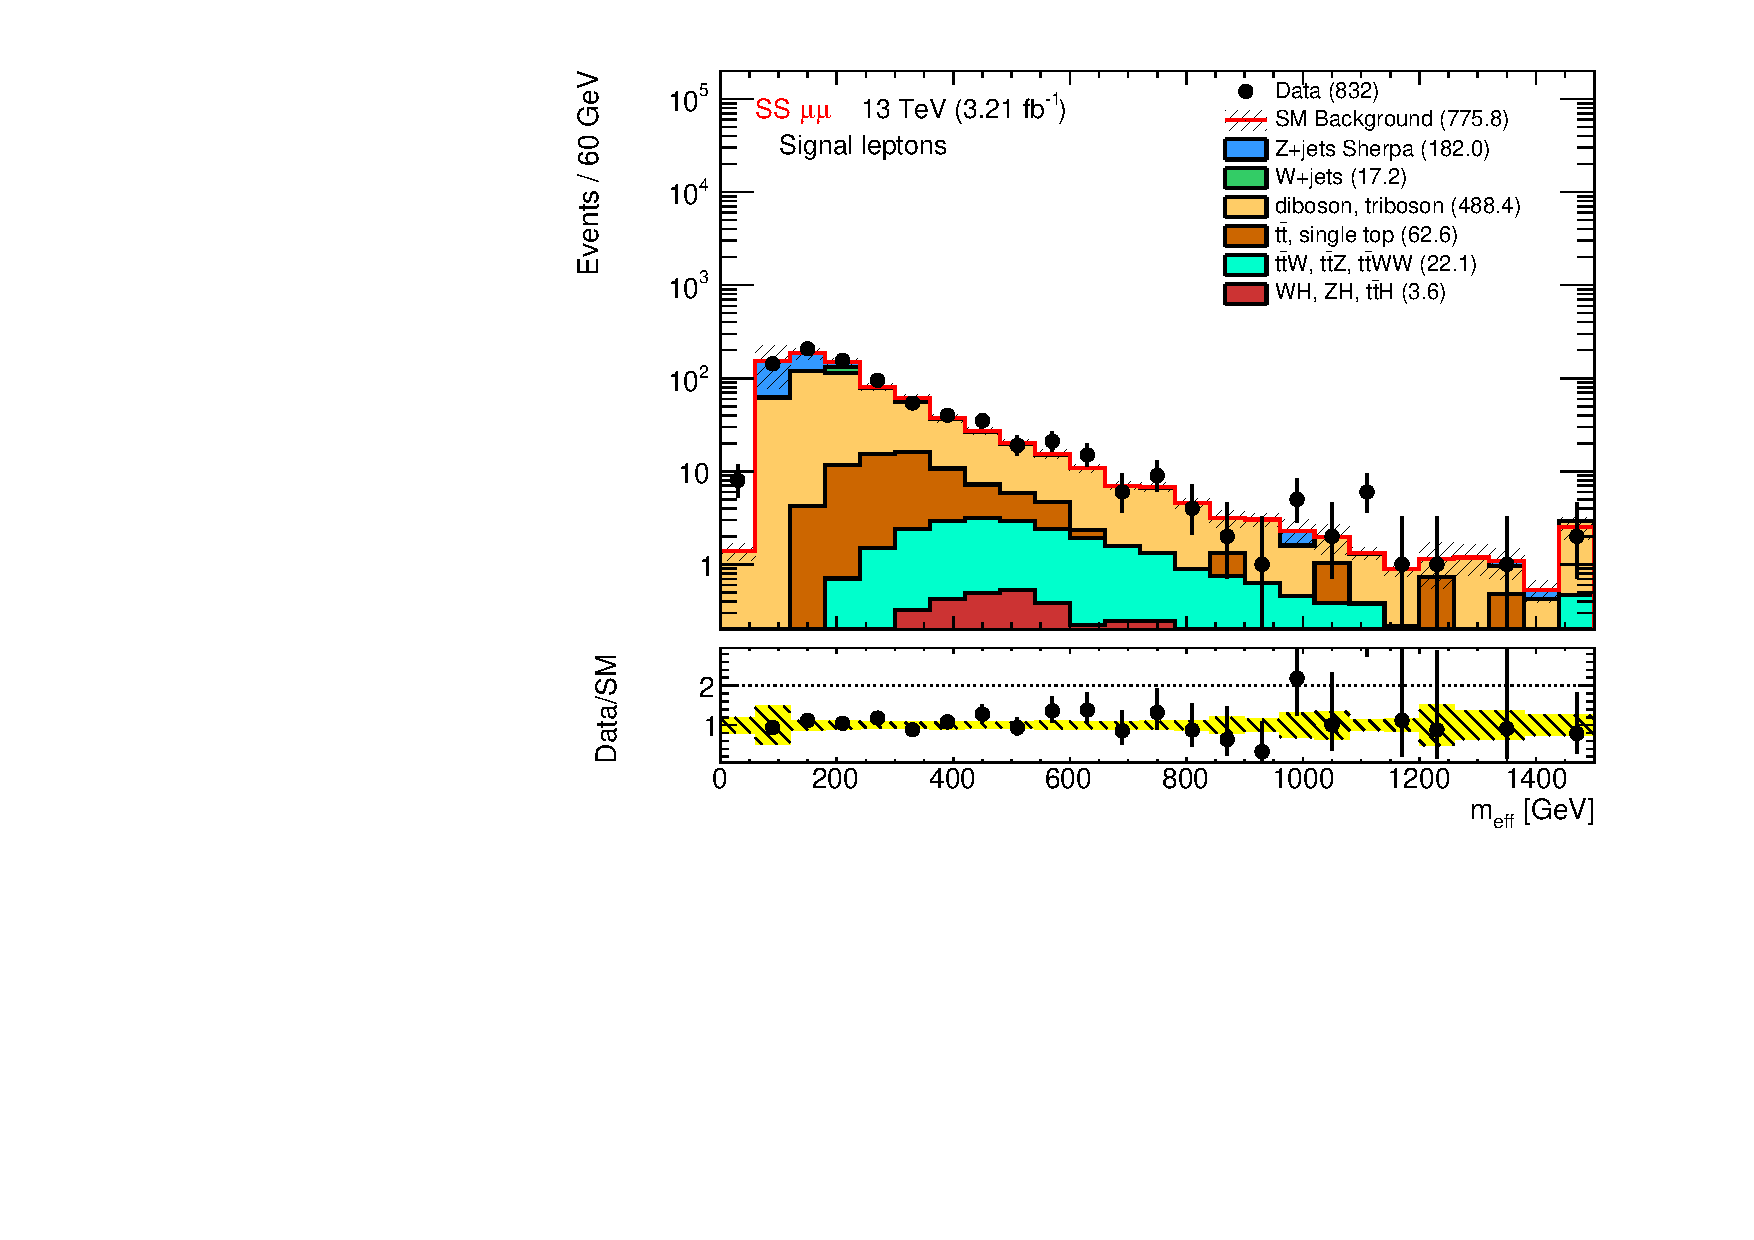
\includegraphics[width=0.49\textwidth]{DATAMC/MEFF_afterlepton_SSmm_0_physics.pdf}}
\caption{Distributions of the $\met$ (left) and effective mass (right) for events selected in the $ee$ (top), $e\mu$ (center) and $\mu\mu$ (bottom) channels. The background contribution is taken directly from MC with no data-driven estimation of the background with fake and non-prompt leptons or charge mis-identification. Only luminosity and MC statistical uncertainties are included.
}
\label{fig:dataMC_metmeff}
\end{figure}

\FloatBarrier

